


%% LyX 1.1 created this file.  For more info, see http://www.lyx.org/.
%% Do not edit unless you really know what you are doing.
\documentclass[twosided,bookman]{book}
\usepackage[T1]{fontenc}
\usepackage[latin1]{inputenc}
\usepackage[english]{babel}
\usepackage{graphicx}
\usepackage{epsfig}
\usepackage{emlines}


\usepackage{amsthm}
\usepackage{amsmath}
\usepackage{graphicx}
%\usepackage{latexcad}
\usepackage{makeidx}

%%%%%%%%%%%%%%%%%%%%%%%%%%%%%% User specified LaTeX commands.
\usepackage[T1]{fontenc}
\usepackage[latin1]{inputenc}
%\usepackage{times}
%\usepackage{helvet}
\usepackage{a4}
\usepackage{pslatex}
\makeindex
\usepackage{color}
\makeatletter
\usepackage{float}
\newfloat{Example}{tb}{lod}[chapter]

\providecommand{\tabularnewline}{\\}
\floatstyle{ruled}
\newfloat{algorithm}{tbp}{loa}[chapter]
\floatname{algorithm}{Algorithm}
%%%%%%%%%%%%%%%%%%%%%%%%%%%%%% LyX specific LaTeX commands.
\providecommand{\LyX}{L\kern-.1667em\lower.25em\hbox{Y}\kern-.125emX\@}
%% Special footnote code from the package 'stblftnt.sty'
%% Author: Robin Fairbairns -- Last revised Dec 13 1996
\let\SF@@footnote\footnote
\def\footnote{\ifx\protect\@typeset@protect
    \expandafter\SF@@footnote
  \else
    \expandafter\SF@gobble@opt
  \fi
}
\expandafter\def\csname SF@gobble@opt \endcsname{\@ifnextchar[%]
  \SF@gobble@twobracket
  \@gobble
}
\edef\SF@gobble@opt{\noexpand\protect
  \expandafter\noexpand\csname SF@gobble@opt \endcsname}
\def\SF@gobble@twobracket[#1]#2{}

%%%%%%%%%%%%%%%%%%%%%%%%%%%%%% Textclass specific LaTeX commands.
 \newenvironment{lyxlist}[1]
   {\begin{list}{}
     {\settowidth{\labelwidth}{#1}
      \setlength{\leftmargin}{\labelwidth}
      \addtolength{\leftmargin}{\labelsep}
      \renewcommand{\makelabel}[1]{##1\hfil}}}
   {\end{list}}
 \newenvironment{lyxcode}
   {\begin{list}{}{
     \setlength{\rightmargin}{\leftmargin}
     \raggedright
     \setlength{\itemsep}{0pt}
     \setlength{\parsep}{0pt}
     \verbatim@font}%
    \item[]}
   {\end{list}}

%% Marginal notes use frequently

\newcommand{\standardnote}[1]{\marginpar{\sc \footnotesize #1}}
\def\pascal{\sc \footnotesize ISO-7185}
\def\standard{\standardnote{\pascal}}
\def\turbo{\standardnote{Turbo}}
\def\extended{\sc \footnotesize ISO-10206}
\def\extendedpascal{\standardnote{\extended}}
\def\vectorpascal{  \standardnote{Vector}}
\def\Unix{          \standardnote{Unix}}
%\def\hyperlink#1#2{\special{html:<a href="\##1">}#2\special{html:</a>}}
%\def\hypertarget#1#2{\special{html:<a name="#1">}#2\special{html:</a>}}
\def\href#1#2{\special{html:<a href="#1">}#2\special{html:</a>}}


\makeatother

\begin{document}


\title{The Glasgow   Pascal Compiler\\ \Large   with vector extensions\footnote{ISBN 978-1-4477-6156-3
,\ Copyright(c) Paul Cockshott, University of Glasgow}}


\author{Paul Cockshott  }

\maketitle


\tableofcontents

%\input intro
\chapter*{Introduction}
  Pascal\cite{Jensen,ISO90a} is an old programming language
whose relative popularity has declined over the years, but like Fortran
and C it lends itself to efficient code generation. Vector Pascal
was first developed by Turner\cite{turner1987vector} and Formella\cite{formella1992spark}.
It supports whole array operations in a manner that is similar to
Fortran 90.
 This manual describes the  Glasgow   Pascal Compiler which supports
 vector extensions similar to those developed by Turner and Formella,
   extensions introduced in ISO Extended Pascal\cite{ISO90} and
   some new extensions.


Modern processors have provision for parallelism in two ways:

\begin{enumerate}\item The Single Instruction-stream
Multiple Data-stream (SIMD\index{SIMD}) model in which a single instruction
causes the same mathematical operation to be carried out on several operands,
or pairs of operands at the same time. The level of parallelism supported ranges
from 2 floating point operations at a time on the older AMD\index{AMD} K\index{K6}6
architecture to 8 floating point operations at a time on the Intel AVX architecture.

\item The provision of multiple cores on one chip which execute parallel instructionsets.
These may all run the same instructionset as on Intel processors, or run
distinct instructionsets as on the IBM Cell chip.
\end{enumerate}
 Whilst
processor architectures are moving towards greater levels of parallelism, the
most widely used programming languages like C\index{C}, Java\index{Java} and
Delphi\index{Delphi} are structured around a model of computation in which
operations take place on a single value at a time. This was appropriate when
processors worked this way, but has become an impediment to programmers seeking
to make use of the performance offered by multi-media instructionsets. The introduction
of SIMD instruction sets\cite{IA32}\cite{Peleg97} to Personal Computers potentially
provided substantial performance increases, but the ability of most programmers
to harness this performance was held back by two factors. The first was the limited
availability of compilers that make effective use of these instructionsets in
a machine independent manner.
The second is the fact that most popular programming languages were designed
on the word at a time model of the classic von Neumann computer.

The Glasgow Pascal Compiler aims to provide an efficient and concise notation for programmers
using Multi-core and SIMD  enhanced CPUs. In doing so it borrows concepts for expressing
data parallelism that have a long history, dating back to Iverson's work on
APL\index{APL} in the early '60s\cite{Iverson62}.

Define a vector of type \emph{T} as having type \( T[] \). Then if we have
a binary operator \( \omega :(T\otimes T)\rightarrow T \), in languages derived
from APL we automatically have an operator \( \omega :(T[]\otimes T[])\rightarrow T[] \)
\(  \). Thus if \( x,y \) are arrays of integers \( k=x+y \) is the array
of integers where \( k_{i}=x_{i}+y_{i} \).

The basic concept is simple, there are complications to do with the semantics
of operations between arrays of different lengths and different dimensions,
but Iverson provides a consistent treatment of these. The most recent languages
to be built round this model are J\index{J}, an interpretive language\cite{Jmanual}\cite{Burke}\cite{Jintro},
and F\cite{Metcalf96} a modernised Fortran\index{Fortran}. In principle though
any language with array types can be extended in a similar way. Iverson's approach
to data parallelism is machine independent. It can be implemented using scalar
instructions or using the SIMD model. The only difference is speed.

Vector Pascal incorporates Iverson's approach to data parallelism. Its aim is
to provide a notation that allows the natural and elegant expression of data
parallel algorithms within a base language that is already familiar to a considerable
body of programmers and combine this with modern compilation techniques.

By an elegant algorithm I mean one which is expressed as concisely as possible.
Elegance is a goal that one approaches asymptotically, approaching but never
attaining\cite{Chaitin}. APL and J allow the construction of very elegant programs,
but at a cost. An inevitable consequence of elegance is the loss of redundancy.
APL programs are as concise, or even more concise than conventional mathematical
notation\cite{Iverson80} and use a special character-set. This makes them hard
for the uninitiated to understand. J attempts to remedy this by restricting
itself to the ASCII character-set, but still looks dauntingly unfamiliar to
programmers brought up on more conventional languages. Both APL and J are interpretive
which makes them ill suited to many of the applications for which SIMD speed
is required. The aim of the vector extensions in the Glasgow Pascal Compiler is to provide the conceptual gains of
Iverson's notation within a framework familiar to imperative programmers.

Pascal\index{Pascal}\cite{Jensen}was chosen as a base language over the alternatives
of C and Java. C was rejected because notations like \texttt{x+y} for \texttt{x}
and \texttt{y} declared as \texttt{int x{[}4{]}}, {\tt y{[}4{]}}, already have the
meaning of adding the addresses of the arrays together. Java was rejected because
of the difficulty of efficiently transmitting data parallel operations via its
intermediate code to a just in time code generator.

Iverson's approach to data parallelism is machine independent. It can be implemented
using scalar instructions or using the SIMD\index{SIMD} model. The only difference
is speed.




%\part{Language Reference Manual\\ \ \\ {\normalsize\em Paul Cockshott}}
%\input man
\chapter{Elements of the language}


\section{Alphabet}
The Glasgow Pascal Compiler accepts files in the UTF-8 encoding of
 Unicode as source. Since ASCII is a subset of this, ASCII files are valid input.

  Pascal programs are made up of letter, digits and special
symbols. The letters digits and special symbols are draw either from a base
 character set or from an extended character set. The base character set is drawn
from ASCII and restricts the letters to be from the Latin alphabet.
The extended character set allows letters from other alphabets.




 The special symbols used in the base alphabet are shown in table\ref{specials} .
\begin{table}

\caption{Special symbols\label{specials}}
\vspace{0.3cm}
{\centering \begin{tabular}{|c|c|c|}
\hline
+&
:&
(\\
\hline
-&
'&
)\\
\hline
{*}&
=&
{[}\\
\hline
/&
<>&
{]}\\
\hline
:=&
<&
\{\\
\hline
.&
<=&
\}\\
\hline
,&
>=&
\textasciicircum{}\\
\hline
;&
>&
..\\
\hline
+:&
@&
{*})\\
\hline
-:&
\$&
({*}\\
\hline
\_&
{*}{*}&
\\
\hline
\end{tabular}\par}\vspace{0.3cm}
\end{table}
\subsection{Extended alphabet}
The extended alphabet is described in section \ref{uni}{Using Unicode with Vector Pascal}.


\section{Reserved words}
\label{resw}
The reserved words are {%\small\bf

   \texttt{{ABS, ADDR, AND, ARRAY,}}

   \texttt{{BEGIN, BYTE2PIXEL,}}

   \texttt{{CASE, CAST, CDECL, CHR, CONST, COS,}}

   \texttt{{ DIV, DO, DOWNTO,}}

   \texttt{{END, ELSE, EXIT, EXTERNAL,}}

   \texttt{{FALSE, FILE, FOR, FUNCTION,}}

   \texttt{{GOTO,}}

   \texttt{{IF, IMPLEMENTATION, IN, INTERFACE, IOTA,}}

   \texttt{{LABEL, LIBRARY, LN,}}

   \texttt{{MAX, MIN, MOD,}}

   \texttt{{NAME, NDX,  NOT,}}

   \texttt{{OF, OR, ORD, OTHERWISE},}

   {\tt PACKED, PERM, PIXEL2BYTE,  POW,  PRED,} \\{\tt PROCEDURE,  PROGRAM,}
{\tt  PROTECTED ,}

   \texttt{{RDU,  RECORD, REPEAT, ROUND,}}

   \texttt{{SET, SHL, SHR, SIN, SIZEOF, STRING, SQRT, SUCC,}}

   \texttt{{TAN, THEN, TO, TRANS, TRUE, TYPE,}}

   \texttt{{VAR,}}

   \texttt{{WITH, WHILE, }}
   \texttt{{UNIT, UNTIL, USES }}
}

Reserved words may be written in either lower case or upper case letters, or
any combination of the two.


\section{Comments}

The comment\index{comment} construct

\texttt{\{\index{}} < any sequence of characters not containing {}``\}{}''
> \texttt{\}}

may be inserted between any two identifiers, special symbols, numbers or reserved
words without altering the semantics or syntactic correctness of the program.
The bracketing pair \texttt{({*} {*})\index{*)}} may substitute for \texttt{\{
\}}. Where a comment starts with \texttt{\{} it continues until the next \texttt{\}}.
Where it starts with \texttt{({*}\index{(*}} it must be terminated by \texttt{{*})}\footnote{%
Note this differs from ISO Pascal which allows a comment starting with \{ to
terminate with {*}) and vice versa.
}.


\section{Identifiers}

Identifiers are used to name values, storage locations, programs, program modules,
types, procedures and functions. An identifier\index{identifier} starts with
a letter followed by zero or more letters, digits or the special symbol \texttt{\_}.
Case is not significant in identifiers.
ISO Pascal allows the Latin letters A-Z   to be used in identifiers.
The Glasgow Pascal Compiler extends this by allowing symbols from the Greek,
Cyrillic, Katakana and Hiragana, or CJK character sets



\section{Literals}


\subsection{Integer numbers}

Integer numbers are formed of a sequence of decimal digits, thus \texttt{1},
\texttt{23}, \texttt{9976} etc, or as hexadecimal\index{hexadecimal} numbers,
or as numbers of any base between 2 and 36. A hexadecimal number takes the form
of a \texttt{\$} followed by a sequence of hexadecimal digits thus \texttt{\$01,
\$3ff, \$5A}. The letters in a hexadecimal number may be upper or lower case
and drawn from the range \texttt{a..f} or \texttt{A..F. }

A based integer\index{integer} is written with the base first followed by a
\# character and then a sequence of letters or digits. Thus \texttt{2\#1101}
is a binary number \texttt{8\#67} an octal\index{octal} number and \texttt{20\#7i}
a base 20 number.

The default precision for integers is 32 bits\footnote{%
The notation used for grammar definition is a tabularised BNF . Each boxed table
defines a production, with the production name in the left column. Each line
in the right column is an alternative for the production. The metasymbol + indicates
one or more repetitions of what immediately preceeds it. The Kleene star {*}
is used for zero or more repetitions. Terminal symbols are in single quotes.
Sequences in brackets {[} {]} are optional.
}.

\vspace{0.3cm}
{\centering \begin{tabular}{|l|l|}
\hline
<digit sequence>&
<digit> +\\
\hline
<decimal integer>&
<digit sequence>\\
\hline
<hex integer>&
`\$'<hexdigit>+\\
\hline
<based integer> &
<digit sequence>'\#'<alphanumeric>+\\
\hline
<unsigned integer>&
<decimal integer>\\
&
<hex integer>\\
&
<based integer>\\
\hline
\end{tabular}
\begin{table}

\caption{The hexadecimal digits of Vector Pascal.}
{\centering \begin{tabular}{ccccccccccccccccc}
\hline
Value&
0&
1&
2&
3&
4&
5&
6&
7&
8&
9&
10&
11&
12&
13&
14&
15\\
\hline
Notation 1&
0&
1&
2&
3&
4&
5&
6&
7&
8&
9&
A&
B&
C&
D&
E&
F\\
%\hline
Notation 2&
0&
1&
2&
3&
4&
5&
6&
7&
8&
9&
a&
b&
c&
d&
e&
f\\
%\hline
\end{tabular}\par}
.
\end{table}
 \par}
\vspace{0.3cm}


\subsection{Real numbers}

Real numbers are supported in floating point notation, thus \texttt{14.7},
 {\tt \ 9.99e5},
{\tt
38E3,} \  {\tt 3.6e-4} are all valid denotations for real\index{real} numbers. The default
precision for real numbers is also 32 bit, though intermediate calculations
may use higher precision. The choice of 32 bits as the default precision is
influenced by the fact that 32 bit floating point vector operations are well
supported in multi-media\index{media} instructions.

\vspace{0.3cm}
{\centering \begin{tabular}{|l|l|}
\hline
<exp>&
`e'\\
&
`E'\\
\hline
<scale factor>&
{[}<sign>{]} <unsigned integer>\\
\hline
<sign>&
`-'\\
&
`+'\\
\hline
<unsigned real>&
<decimal integer> `.' <digit sequence>\\
&
<decimal integer>` .' <digit sequence> <exp><scale factor> \\
&
<decimal integer><exp> <scale factor>\\
\hline
\end{tabular}\par}
\vspace{0.3cm}


\subsubsection{Fixed point numbers}

In the Glasgow Pascal Compiler output code pixels\index{pixels} are represented as signed fixed point
fractions in the range -1.0 to 1.0. Within this range, fixed point literals
have the same syntactic form as real numbers.


\subsection{Character strings}

Sequences of characters enclosed by quotes are called literal\index{literal}
strings. Literal strings\index{strings} consisting of a single character are
constants of the standard type char. If the string is to contain a quote character
this quote character must be written twice.

\texttt{\small 'A' 'x' 'hello' 'John''s house'}{\small \par}

are all valid literal strings. The allowable characters in literal strings are
any of the Unicode characters above u0020. The character strings must be input
to the compiler in UTF-8 format.




\chapter{Declarations}

 Pascal is a language supporting nested declaration\index{declaration}
contexts. A declaration context is either a program context, and unit interface
or implementation context, or a procedure or function context. A resolution
context determines the meaning of an identifier. Within a resolution context,
identifiers can be declared to stand for constants, types, variables, procedures
or functions. When an identifier is used, the meaning taken on by the identifier
is that given in the closest containing resolution context. Resolution contexts
are any declaration context or a \texttt{with} statement context. The ordering
of these contexts when resolving an identifier is:

\begin{enumerate}
\item The declaration context identified by any \texttt{with} statements which nest
the current occurrence of the identifier. These \texttt{with} statement contexts
are searched from the innermost to the outermost.
\item The declaration context of the currently nested procedure\index{procedure}
declarations. These procedure contexts are searched from the innermost to the
outermost.
\item The declaration context of the current unit\index{unit} or program\index{program}.
\item The interface declaration contexts of the units mentioned in the use list of
the current unit or program. These contexts are searched from the rightmost
unit mentioned in the use list to the leftmost identifier in the use list.
\item The interface declaration context of the System\index{System} unit.
\item The pre-declared identifiers of the language.
\end{enumerate}



\section{Constants}

A constant definition introduces an identifier as a synonym for a constant.

\vspace{0.3cm}
{\centering \begin{tabular}{|l|l|}
\hline
<constant declaration>&
<identifier>=<expression>\\
&
<identifier>':'<type>'='<typed constant>\\
\hline
\end{tabular}\par}
\vspace{0.3cm}

Constants can be simple constants or typed constants. A simple constant must
be a constant expression whose value is known at compile time. This restricts
it to expressions for which all component identifiers are other constants, and
for which the permitted operators\index{operators} are given in table\ref{MMConst}
. This restricts simple constants to be of scalar or string types.


\begin{table}

\caption{The operators permitted in  constant expressions.\label{MMConst}}
{\centering \begin{tabular}{|c|c|c|c|c|c|c|c|c|c|}
\hline
+&
-&
{*}&
/&
div&
mod&
shr&
shl&
and&
or\\
\hline
\end{tabular}\par}\end{table}
Typed constants provide the program with initialised variables which may hold
array types.

\vspace{0.3cm}
{\centering \begin{tabular}{|l|l|}
\hline
<typed constant>&
<expression>\\
&
<array constant>\\
\hline
\end{tabular}\par}
\vspace{0.3cm}


\subsection{Array constants}

Array constants are comma separated lists of constant expressions enclosed by
brackets. Thus

\texttt{tr:array{[}1..3{]} of real =(1.0,1.0,2.0);}

is a valid array constant declaration, as is:

{\small
\texttt{t2:array{[}1..2,1..3{]} of real=((1.0,2.0,4.0),(1.0,3.0,9.0));}}

The array constant\index{constant}\index{array constant} must structurally
match the type\index{type} given to the identifier. That is to say it must
match with respect to number of dimensions, length of each dimension, and type
of the array elements.

\vspace{0.3cm}
{\centering \begin{tabular}{|l|l|}
\hline
<array constant>&
'(' <typed constant> {[},<typed constant>{]}{*} ')'\\
\hline
\end{tabular}\par}
\vspace{0.3cm}


\subsection{Pre-declared constants\index{constants}}

\begin{lyxlist}{00.00.0000}
\item [\texttt{maxint\index{maxint}}]The largest supported integer value.
\item [\texttt{pi\index{pi}}] A real numbered approximation to $ \pi  $
\item [\texttt{maxchar\index{maxchar}}] The highest character in the character set.
\item [\texttt{maxstring\index{maxstring}}]The maximum number of characters allowed
in a string.
\item [\texttt{maxreal\index{maxreal}}]The highest representable real.
\item [\texttt{minreal\index{minreal}}]The smallest representable positive real number.
\item [\texttt{epsreal\index{epsreal}}]The smallest real number which when added
to 1.0 yields a value distinguishable from 1.0.
\item [\texttt{maxdouble\index{maxdouble}}]The highest representable double precision
real number.
\item [\texttt{mindouble\index{mindouble}}]The smallest representable positive double
precision real number.
\item [\texttt{complexzero\index{complexzero}}]A complex number with zero real and
imaginary parts.
\item [\texttt{complexone}\index{complexone}]A complex number with real part 1 and
imaginary part 0.
\end{lyxlist}

\section{Labels}

Labels are written as digit sequences. Labels must be declared before they are
used. They can be used to label the start of a statement and can be the destination
of a \texttt{goto\index{goto}} statement. A \texttt{goto} statement must have
as its destination a label\index{label} declared within the current innermost
declaration context. A statement can be prefixed by a label followed by a colon.

Example

\texttt{label 99;}

\texttt{begin read(x); if x>9 goto 99; write(x{*}2);99: end;}


\section{Types}

A type declaration determines the set of values that expressions of this type
may assume and associates with this set an identifier.

\vspace{0.3cm}
{\centering \begin{tabular}{|l|l|}
\hline
<type>&
<simple type>\\
&
<structured type>\\
&
<pointer type>\\
\hline
<type definition>&
<identifier>'='<type> \\
\hline
\end{tabular}\par}
\vspace{0.3cm}


\subsection{Simple types}

Simple types are either scalar, standard, subrange or dimensioned types.

\vspace{0.3cm}
{\centering \begin{tabular}{|l|l|}
\hline
<simple type>&
<scalar type>\\
&
<integral type>\\
&
<subrange type>\\
&
<dimensioned type>\\
&
<floating point type>\\
\hline
\end{tabular}\par}
\vspace{0.3cm}


\subsubsection{Scalar types}

A scalar\index{scalar} type\index{type} defines an ordered set of identifier
by listing these identifiers. The declaration takes the form of a comma separated
list of identifiers enclosed by brackets. The identifiers in the list are declared
simultaneously with the declared scalar type to be constants of this declared
scalar type. Thus
\begin{verbatim}
colour = (red,green,blue);
day=(monday,tuesday,wednesday,thursday,
     friday,saturday,sunday);
\end{verbatim}
are valid scalar type declarations.


\subsubsection{Standard types}\label{auxtypes}

The following types are provided as standard in Vector Pascal:
\begin{table}

\caption{Categorisation of the standard types.}
{\centering \begin{tabular}{|l|l|}
\hline
type&
category\\
\hline
\hline
real&
floating point\\
\hline
double&
floating point\\
\hline
byte&
integral\\
\hline
pixel&
fixed point\\
\hline
shortint&
integral\\
\hline
word&
integral\\
\hline
integer&
integral\\
\hline
cardinal&
integral\\
\hline
boolean&
scalar\\
\hline
char&
scalar\\
\hline
\end{tabular}\par}\end{table}


\begin{lyxlist}{00.00.0000}
\item [\texttt{integer\index{integer}}]The numbers are in the range -maxint to +maxint.
\item [\texttt{real\index{real}}]These are a subset of the reals constrained by the
IEEE 32 bit floating point format.
\item [\texttt{double\index{double}}]These are a subset of the real numbers constrained
by the IEEE\index{IEEE} 64 bit floating point format.
\item [\texttt{pixel\index{pixel}}]These are represented as fixed\index{fixed} point\index{point}
binary\index{binary} fractions\index{fractions} in the range -1.0 to 1.0.
\item [\texttt{boolean\index{boolean}}]These take on the values \texttt{(false\index{false},true\index{true})}
which are ordered such that \texttt{true>false}.
\item [\texttt{char\index{char}}]These include the characters from \texttt{chr(0)}
to \texttt{charmax}\index{charmax}. All the allowed characters for string literals
are in the type char, but the character-set may include other characters whose
printable form is country specific.
\item [\texttt{pchar}\index{pchar}]Defined as \texttt{\textasciicircum{}char}.
\item [\texttt{byte\index{byte}}]These take on the positive integers between 0 and
255.
\item [\texttt{shortint\index{shortint}}]These take on the signed values between
-128 and 127.
\item [\texttt{word\index{word}}]These take on the positive integers from 0 to 65535.
\item [\texttt{cardinal\index{cardinal}}]These take on the positive integers form
0 to 4292967295, i.e., the most that can be represented in a 32 bit unsigned
number.
\item [\texttt{longint\index{longint}}]A 32 bit integer, retained for compatibility
with Turbo Pascal.
\item [\texttt{int\index{int64}64}]A 64 bit integer.
\item [\texttt{complex\index{complex}}]A complex number with the real and imaginary
parts held to 32 bit precision.
\end{lyxlist}

\subsubsection{Subrange types}

A type may be declared as a subrange\index{subrange} of another scalar\index{scalar}
or integer\index{integer} type by indicating the largest and smallest value
in the subrange. These values must be constants known at compile time.

\vspace{0.3cm}
{\centering \begin{tabular}{|l|l|}
\hline
<subrange type>&
<constant> '..' <constant>\\
\hline
\end{tabular}\par}
\vspace{0.3cm}

Examples: 1..10, 'a'..'f', monday..thursday.


\subsubsection{Pixels}

The \emph{conceptual model} of pixels in Vector Pascal is that they are real
numbers in the range $ -1.0..1.0 $. As a signed representation it lends itself
to subtraction. As an unbiased representation, it makes the adjustment of contrast
easier. For example, one can reduce contrast 50\% simply by multiplying an image
by 0.5 \footnote{%
When pixels are represented as integers in the range 0..255, a 50\% contrast
reduction has to be expressed as $ ((p-128)\div 2)+128 $.
}. Assignment to pixel variables in Vector Pascal is defined to be saturating
- real numbers outside the range $ -1..1 $ are clipped to it. The multiplications
involved in convolution operations fall naturally into place.

The \emph{implementation model} of pixels used in Vector Pascal is of 8 bit
signed integers treated as fixed point binary fractions. All the conversions
necessary to preserve the monotonicity of addition, the range of multiplication
etc, are delegated to the code generator which, where possible, will implement
the semantics using efficient, saturated multi-media arithmetic instructions.


\subsubsection{Dimensioned types}

These provide a means by which floating point types can be specialised to represent
dimensioned numbers as is required in physics calculations. For example:

\texttt{kms =(mass,distance,time);}

\texttt{meter=real of distance;}

\texttt{kilo=real of mass;}

\texttt{second=real of time;}

\texttt{newton=real of mass {*} distance {*} time POW -2;}

\texttt{meterpersecond = real of distance {*}time POW -1;}

The grammar is given by:

\vspace{0.3cm}
{\centering \begin{tabular}{|l|l|}
\hline
<dimensioned type>&
<real type> <dimension >{[}'{*}' <dimension>{]}{*}\\
\hline
<real type>&
'real'\\
&
'double'\\
\hline
<dimension>&
<identifier> {[}'POW' {[}<sign>{]} <unsigned integer>{]}\\
\hline
\end{tabular}\par}
\vspace{0.3cm}

The identifier\index{identifier} must be a member of a scalar type, and that
scalar type is then referred to as the basis space of the dimensioned type.
The identifiers of the basis\index{basis} space are referred to as the dimensions
of the dimensioned type\index{type}. Associated with each dimension of a dimensioned
type there is an integer number referred to as the power of that dimension.
This is either introduced explicitly at type declaration time, or determined
implicitly for the dimensional type of expressions.

A value of a dimensioned type is a dimensioned value. Let $ \log _{d}t $
of a dimensioned type $ t $ be the power to which the dimension $ d $
of type $ t $ is raised. Thus for $ t= $newton in the example above, and
$ d= $time, $ \log _{d}t=-2 $

If $ x $ and $ y $ are values of dimensioned\index{dimensioned} types
$ t_{x} $and $ t_{y} $respectively, then the following operators are only
permissible if $ t_{x}=t_{y} $

\vspace{0.3cm}
{\centering \begin{tabular}{|c|c|c|c|c|c|c|c|}
\hline
+&
-&
<&
>&
<>&
=&
<=&
>=\\
\hline
\end{tabular}\par}
\vspace{0.3cm}

For + and -, the dimensional\index{dimensional} type of the result is the same
as that of the arguments. The operations

\vspace{0.3cm}
{\centering \begin{tabular}{|l|l|}
\hline
{*}&
/\\
\hline
\end{tabular}\par}
\vspace{0.3cm}

are permitted if the types $ t_{x} $and $ t_{y} $ share the same basis
space, or if the basis space of one of the types is a subrange of the basis
space of the other.

The operation \texttt{POW} is permitted between dimensioned types and integers.


\paragraph*{Dimension deduction rules}

\begin{enumerate}
\item If $ x=y*z $ for $ x:t_{1},y:t_{2},z:t_{3} $ with basis space $ B $
then


 $$ \forall _{ d \in B } \log_dt_1= \log_dt_2+\log_dt_3 $$

\item If $ x=y/z $ for $ x:t_{1},y:t_{2},z:t_{3} $ with basis space $ B $
then


$$ \forall_{d \in B}\log _{d}t_{1}=\log _{d}t_{2}-\log _{d}t_{3} $$

\item If $ x=y $ \texttt{POW} $ z $ for $ x:t_{1},y:t_{2},z:integer $ with
basis space for $ t_{2} $, $ B $ then


$$ \forall_{d\in B}\log _{d}t_{1}=\log _{d}t_{2}\times z $$.

\end{enumerate}

\subsection{Structured types}


\subsubsection{Static Array\index{array}\index{array, static} types}

An array type is a structure consisting of a fixed number of elements all of
which are the same type. The type of the elements is referred to as the element
type. The elements of an array value are indicated by bracketed indexing expressions.
The definition of an array\index{array} type\index{type} simultaneously defines
the permitted type of indexing expression and the element type.

The index\index{index} type\index{type} of a static\index{static} array\index{array, static}
must be a scalar\index{scalar} or subrange\index{subrange} type. This implies
that the bounds of a static array are known at compile time.

\vspace{0.3cm}
{\centering \begin{tabular}{|l|l|}
\hline
<array type>&
'array' '{[}' <index type>{[},<index type>{]}{*} '{]}' 'of' <type>\\
\hline
<index type>&
<subrange type>\\
&
<scalar type>\\
&
<integral type>\\
\hline
\end{tabular}\par}
\vspace{0.3cm}

Examples

\texttt{array{[}colour{]} of boolean;}

\texttt{array{[}1..100{]} of integer;}

\texttt{array{[}1..2,4..6{]} of byte;}

\texttt{array{[}1..2{]} of array{[}4..6{]} of byte;}

The notation {[}\emph{b,c}{]} in an array declaration is shorthand for the notation
{[}\emph{b}{]} \texttt{of array} {[} \emph{c} {]}. The number of dimensions of an
array type is referred to as its rank. Scalar types have rank 0.


\subsubsection{String types}

A string\index{string} type denotes the set of all sequences of characters
up to some finite length and must have the syntactic form:

\vspace{0.3cm}
{\centering \begin{tabular}{|l|l|}
\hline
<string-type>&
'string{[}' <integer constant>'{]}'\\
&
'string'\\
&'string{(}' <ingeger constant>'{)}'\\
\hline
\end{tabular}\par}
\vspace{0.3cm}

the integer constant indicates the maximum number of characters that may be
held in the string type. The maximum number of characters that can be held in
any string is indicated by the pre-declared constant \texttt{maxstring}. The
type \texttt{string} is shorthand for \texttt{string{[}maxstring{]}}.


\subsubsection{Record types}

A record type defines a set of similar data structures. Each member of this
set, a record instance, is a Cartesian product of number of components or \emph{fields}
specified in the record\index{record} type definition. Each field has an identifier
and a type. The scope of these identifiers is the record itself.

A record type may have as a final component a \emph{variant\index{variant}
part}. The variant part, if a variant part exists, is a union of several variants,
each of which may itself be a Cartesian product of a set of fields. If a variant
part exists there may be a tag field whose value indicates which variant is
assumed by the record instance.

All field identifiers even if they occur within different variant parts, must
be unique within the record type.

\vspace{0.3cm}
{\centering \begin{tabular}{|l|l|}
\hline
<record type>&
'record' <field list> 'end'\\
\hline
<field list>&
<fixed part>\\
&
<fixed part>';' <variant part>\\
&
<variant part>\\
\hline
<fixed part>&
<record section> {[} ';' <record section.{]}{*}\\
\hline
<record section>&
<identifier>{[}',' <identifier>{]}{*} ':' <type>\\
&
<empty>\\
\hline
<variant part>&
'case' {[}<tag field> ':'{]} <type identifier> 'of'<variant>{[}';' <variant>{]}{*}\\
\hline
<variant>&
<constant> {[}',' <constant>{]}{*}':' '(' <field list> ')'\\
&
<empty>\\
\hline
\end{tabular}\par}
\vspace{0.3cm}


\subsubsection{Set types}

A set\index{set} type defines the range of values which is the power-set of
its base type. The base type must be an ordered type, that is a type on which the
operations $<$, $=$ and $>$ are defined\footnote{ ISO Pascal requires
the base type to be a scalar type, a character type, integer
type or a subrange thereof. When the base type is one of these, Vector Pascal implements
the set using bitmaps. When the type is other than these, balanced binary trees are used.
It is strongly recomended that use be made of Boehm garbage collector (see section \ref{garbage}) if non-bitmapped
sets are used in a program.}.
Thus sets may be declared whose base types are characters, numbers, ordinals, or strings. Any user
defined type on which the comparison operators have been defined can also be the base type
of a set.

\vspace{0.3cm}
{\centering \begin{tabular}{|l|l|}
\hline
<set type>&
'set' 'of' <base type>\\
\hline
\end{tabular}\par}
\vspace{0.3cm}


\subsection{Dynamic\index{Dynamic} types}

Variables declared within the program are accessed by their identifier. These
variables exist throughout the existence of the scope within which they are
declared, be this unit, program or procedure. These variables are assigned storage
locations whose addresses, either absolute or relative to some register, can
be determined at compile time. Such locations a referred to as static\index{static}\footnote{%
The Pascal concept of static variables should not be equated with the notion
of static variables in some other languages such as C or Java. In Pascal a variable
is considered static if its offset either relative to the stack base or relative
to the start of the global segment can be determined at compile/link time. In
C a variable is static only if its location relative to the start of the global
segment is known at compile time.
}. Storage locations may also be allocated dynamically. Given a type \texttt{t},
the type of a pointer\index{pointer} to an instance of type \texttt{t} is \texttt{\textasciicircum{}t}.

A pointer of type \texttt{\textasciicircum{}t} can be initialised to point to
a new store location on the heap of type t by use of the built in procedure \texttt{new}.
Thus if \texttt{p:\textasciicircum{}t},

\texttt{new(p);}

causes \texttt{p} to point at a store location of type \texttt{t}. The space
can be freed by calling {\tt dispose(p)}. If garbage collection
is enabled at compile time, freeing of store is automatic. By default
garbage collection is off.


\subsubsection{Pointers to dynamic\index{dynamic}\index{dynamic array} arrays\index{array, dynamic}\index{array}}

The types pointed to by pointer types can be any of the types mentioned so far,
that is to say, any of the types allowed for static\index{static} variables.
In addition however, pointer types can be declared to point at dynamic arrays.


A dynamic array is an array whose bounds are determined at run time.

Pascal\index{Pascal90} 90\cite{ISO90} introduced the notion of schematic or
parameterised types as a means of creating dynamic arrays. Thus where \texttt{r}
is some integral or ordinal type one can write

\texttt{type z(a,b:r)=array{[}a..b{]} of t;}

If \texttt{p:\textasciicircum{}z}, then

\texttt{new(p,n,m)}

where \texttt{n,m:r} initialises \texttt{p} to point to an array of bounds \texttt{n..m}.
The bounds of the array can then be accessed as \texttt{p\textasciicircum{}.a,
p\textasciicircum{}.b}. In this case {\tt a, b} are the formal parameters of
the array type. Vector Pascal currently only allows
parameterised types to be allocated on the heap via {\tt new}. The extended form of the procedure {\tt new } must be passed an actual
parameter for each formal parameter in the array type.
\begin{figure}
 \includegraphics[scale=0.75]{sumsq.png}
 \caption{How dynamic arrays are implemented}
 \end{figure}
Dynamic array types can be used to allow slices of arrays to be passed as parameters to functions
as shown here:
\begin{verbatim}
type vector(a:integer)=array[0..a] of integer;
    pv=^vector;
    function sumsq (  var v:vector):integer;
    var total,i:integer;
    begin
         total:=0;
         for i:=0 to v.a do total:= total+ v[i]*v[i];
         sumsq:=total;
     end;
var vp:pv;
begin
    new (vp,6);
    vp^:=iota[0];
    writeln(sumsq (vp^[3..5]));
\end{verbatim}
When using schematic array types in this way, one must take care to
pass the array as a var parameter. This is because,  unlike static arrays which are simply copied on the
stack when passed as value parameters, the compiler
can not pre-allocate space on the call stack for a schematic array.
This means that you must pass them by reference as a var parameter.
Schematic arrays
are implemented as descriptors to the actual arrays.

\subsubsection{Aliases}\index{alias}
In addition to being able to implicitly alias parts of arrays when passing them to
procedures the same effect can be achieved by the built in procedure {\tt alias}.
\begin{verbatim}
type vector(a:integer)=array[1..a] of integer;
     pv=^vector;
var vp,p:pv;
begin
    new (vp,6);
    vp^:=iota[0];
    alias(p,vp^[3..5]);
    (* now  vp^[3]= p^[1]  *)
\end{verbatim}
The {\tt alias} procedure takes as its first parameter a pointer to
a schematic array, and as its second paramter an array section.
The types of the schematic array an the array section must match.
It initialises the array pointer to point to a new descriptor on
the heap of the array section. This new descriptor occupies heap
space, and if gargage collection is not enabled it should be discarded
using {\tt dispose} when it it no longer needed.\index{dispose}
\subsubsection{Delphi style arrays}

Vector Pascal also allows the use of Delphi style declarations for dynamic arrays. Thus one
can declare:
\begin{verbatim}
type vector = array of real;
     matrix = array of array of real;
\end{verbatim}
The size of such arrays has to be explicitly initialised at runtime by a call to the
library procedure {\tt setlength}.
Thus one might have:
\begin{verbatim}
function readtotal:real;
var len:integer;
    v:vector;
begin
 readln(len);
 setlength(v,len);
 readln(v);
 readtotal := \+ v;
end;
\end{verbatim}
The function {\tt readtotal} reads the number of elements in a vector from
the standard input. It then calls {\tt setlength} to initialise the vector length.
Next it reads in the vector and computes its total using the reduction operator \verb{ \+{.

Delphi style arrays are implemented as pointers.
In the example, the variable {\tt v} denotes an array of reals not a pointer
to an array of reals. That is to say you do not have to explicitly dereference {\tt v}
using \verb@ ^ @.
 However, since the array size is not known at compile time
{\tt setlength} will allocate space for the array  on the heap not in the local stack
frame. The use of {\tt setlength} is thus restricted to programs which have been
compiled with the garbage collection flag enabled (see section \ref{BOEHM}).
The procedure {\tt setlength } must be passed a parameter for each dimension of
the dynamic array. The bounds of the array {\tt a} formed by {\tt \\ setlength(a,i,j,k)\\}
would then be {\tt 0..i-1, 0..j-1, 0..k-1}.

\subsubsection{Low \index{low} and High \index{high}}
The built in functions {\tt low } and {\tt high} return the lower and upper bounds
of an array respectively. They work with both static and dynamic arrays.
Consider the following examples.
\begin{verbatim}
program arrays;
type  z(a,b:integer)=array[a..b] of real;
      vec = array of real;
      line= array [1..80] of char;
      matrix = array of array of real;
var i:^z; v:vec; l:line; m:matrix;
begin
 setlength(v,10);setlength(m,5,4);
 new(i,11,13);
 writeln(low(v), high(v));
 writeln(low(m), high(m));
 writeln(low(m[0]),high(m[0]));
 writeln(low(l),high(l));
 writeln(low(i^),high(i^));
end.
\end{verbatim}
would print
\begin{verbatim}
           0           9
           0           4
           0           3
           1          80
          11          13
\end{verbatim}
\subsection{Class types}
The simplest form of class type is similar to a record.
Consider the following example:
\begin{verbatim}
type  A= class
          f1:integer;
         end;
         B=class(A)
         f2:real;
         end;
var c1,anA:A;c2:B;d:boolean;
begin
   new(c1);
   new(c2);
   c1^.f1:=1;
   c1.f1:=2;
   anA:=c2;
   c2.f1:= 1+ c1^.f1;
   d:=(c1.f1+c2.f1)<>5 ;
\end{verbatim}
At the end of the above code {\tt d} is false.
The example declares two classes {\tt A} with field {\tt f1}
and class {\tt B} which has fields {\tt f1} and {\tt f2}.
The construct {\tt (A) } in the header of {\tt B} indicates
that it inherits all the fields of {\tt A}.


When a variable of a class\index{class} type is explicitly declared, what is actually being declared
is a pointer to an instance of that class. The pointer must be initialised using {\tt new}
as shown. Fields can be accessed using the same {\tt  .} notation used for record fields except
that for classes the \verb@ ^ @ for pointer dereference can be optionally elided.
The ability to elide the pointer dereference operator for class instances is a feature inherited from
the syntax of Delphi.

Note that in the example the variable {\tt anA} must point to an instance of class {\tt A}
but it is valid to assign to it a pointer to an instance of class {\tt B} since an
instance of class {\tt B} contains all the fields that a class {\tt A} instance contains.

Classes can contain procedure and function header declarations as shown in the next example.
The function or procedure itself must be declared lower down within the scope in which
the class itself is declared\footnote{This is analogous to the way interfaces of units may
contain procedure headers ( see Chapter \ref{progunit} ).}. When declaring a procedure
belonging to a class, the name of the procedure must be prepended by the class name followed by a
full-stop.
\begin{verbatim}
program classdemo;
type  A= class
         f1:integer;
         function hello:boolean;
         end;
var c1:A;
function A.hello:boolean;
begin
  writeln('hello from class A with a method');
  hello:=true;
end;
\end{verbatim}
The functions or procedures declared within a class can be invoked
by prepending the function or procedure name with the class instance variable
followed by a fullstop:
\begin{verbatim}
begin
   new(c1);
   c1.f1:=2;
   if not c1.hello then
   writeln('this will never be written')
end.

\end{verbatim}
Procedures or functions implementing headers declared within a class have access to the fields
of the class instance that they belong to. Within the procedure, names declared in the class
appear to be in an immediately enclosing scope as shown below.
\begin{verbatim}
type  A= class
         f1:integer;
         function hello:boolean;
         end;
var c1:A;
    i:integer;
function a.hello:boolean;
begin
  hello:=f1=i;
end;
begin
   new(c1);
   c1.f1:=2;
   i:=c1.f1;
   if not  c1.hello then { something is very wrong }
\end{verbatim}
The function {\tt hello} in {\tt A} has access to the field {\tt f1}.

If a class {\tt B} has a procedure with the same name as one in
class {\tt A} then the procedure in {\tt B} will override the
one in {\tt A} as shown:
\begin{verbatim}
type  A= class
         f1:integer;
         function hello:boolean;
         end;
     B= class (A)
         f2:integer;
         function hello:boolean;
         end;
var c1:b;
    i:integer;
function A.hello:boolean;
begin
  writeln('this will not be called ');
  hello:=false;
end;
function B.hello:boolean;
begin
   hello:=f1=i;
end;
begin
   new(c1);
   c1.f1:=2;
   i:=c1.f1;
   if  c1.hello then
   writeln('inheritance works as expected');
end.
\end{verbatim}
\subsubsection{Protected, Public, Private, Virtual}
The above keywords from Delphi are accepted by the Vector Pascal compiler but ignored.
In essence all procedures and functions in classes are assumed to be virtual in the Delphi sense.
\subsection{File types}

A type may be declared to be a file of a type. This form of definition is kept
only for backward compatibility. All file types are treated as being equivalent.
A file type corresponds to a handle to an operating system file. A file variable
must be associated with the operating system file by using the procedures \texttt{assign,
rewrite, append}, and \texttt{reset} provided by the system unit. A pre-declared
file type \texttt{text} exists.

Text files are assumed to be in Unicode UTF-8 format. Conversions are performed between
the internal representation of characters and UTF-8 on input/output from/to a text file.

\section{Variables\index{Variables}}

Variable declarations consist of a list of identifiers denoting the new variables,
followed by their types.

\vspace{0.3cm}
{\centering \begin{tabular}{|l|l|}
\hline
<variable declaration>&
<identifier> {[}',' <identifier>{]}{*} ':' <type><extmod>\\
\hline
\end{tabular}\par}
\vspace{0.3cm}

Variables are abstractions over values. They can be either simple identifiers,
components or ranges of components of arrays, fields of records or referenced
dynamic variables.

\vspace{0.3cm}
{\centering \begin{tabular}{|l|l|}
\hline
<variable>&
<identifier>\\
&
<indexed variable>\\
&
<indexed range>\\
&
<field designator>\\
&
<referenced variable>\\
\hline
\end{tabular}\par}
\vspace{0.3cm}

Examples

\texttt{x,y:real;}

\texttt{i:integer;}

\texttt{point:\textasciicircum{}real;}

\texttt{dataset:array{[}1..n{]}of integer;}

\texttt{twoDdata:array{[}1..n,4..7{]} of real;}


\subsection{External Variables}

A variable may be declared to be external by appending the external modifier.

\vspace{0.3cm}
{\centering \begin{tabular}{|l|l|}
\hline
<extmod>&
';' 'external' 'name' <stringlit>\\
\hline
\end{tabular}\par}
\vspace{0.3cm}

This indicates that the variable is declared in a non Vector Pascal external
library. The name by which the variable is known in the external library is
specified in a string literal.

Example

\texttt{count:integer; external name '\_count';}


\subsection{Entire Variables}\label{entire}

An entire variable is denoted by its identifier. Examples \texttt{x,y,point},


\subsection{Indexed Variables}

A component of an \emph{n} dimensional array variable is denoted by the variable
followed by \emph{n} index expressions in brackets.

\vspace{0.3cm}
{\centering \begin{tabular}{|l|l|}
\hline
<indexed variable>&
<variable>'{[}' <expression>{[}','<expression>{]}{*} '{]}'\\
\hline
\end{tabular}\par}
\vspace{0.3cm}

The type of the indexing expression must conform to the index type of the array
variable. The type of the indexed variable is the component type of the array.

Examples

\texttt{twoDdata{[}2,6{]}}

\texttt{dataset{[}i{]}}

Given the declaration

\texttt{a=array{[}p{]} of q}

then the elements of arrays of type \texttt{a}, will have type \texttt{q} and
will be identified by indices\index{indices} of type \texttt{p} thus:

\texttt{b{[}i{]}}

where \texttt{i:p}, \texttt{b:a}.

Given the declaration

\texttt{z = string{[}x{]}}

for some integer x \texttt{$ \leq  $maxstring}, then the characters within
strings\index{strings} of type \texttt{z} will be identified by indices in
the range \texttt{1..x,} thus:

\texttt{y{[}j{]}}

where \texttt{y:z}, \texttt{j:1..x}.


\subsubsection{Indexed Ranges}

A range of components of an array variable are denoted by the variable followed
by a range expression in brackets.

\vspace{0.3cm}
{\centering \begin{tabular}{|l|l|}
\hline
<indexed range>&
<variable> '{[}' <range expression>{[}',' <range expression>{]}{*} '{]}'\\
\hline
<range expression>&
<expression> '..' <expression>\\
\hline
\end{tabular}\par}
\vspace{0.3cm}

The expressions within the range\index{range} expression must conform to the
index type of the array variable. The type of a range expression \texttt{a{[}i..j{]}}
where \texttt{a: array{[}p..q{]} of t} is \texttt{array{[}0..j-i{]} of t.}

Examples:

\texttt{dataset{[}i..i+2{]}:=blank;}

\texttt{twoDdata{[}2..3,5..6{]}:=twoDdata{[}4..5,11..12{]}{*}0.5;}

Subranges\index{Subranges} may be passed in as actual parameters to procedures
whose corresponding formal parameters\index{parameters} are declared as variables
of a schematic\index{schematic} type. Hence given the following declarations:

\texttt{type image(miny,maxy,minx,maxx:integer)=array{[}miny..maxy,minx..maxx{]}
of byte;}

\texttt{procedure invert(var im:image);begin im:=255-im; end;}

\texttt{var screen:array{[}0..319,0..199{]} of byte;}

then the following statement would be valid:

\texttt{invert(screen{[}40..60,20..30{]});}


\subsubsection{Indexing arrays with arrays}

If an array\index{array} variable occurs on the right hand side of an assignment
statement, there is a further form of indexing possible. An array may be indexed
by another array. If \texttt{x:array{[}t0{]} of t1} and \texttt{y:array{[}t1{]}
of t2}, then \texttt{y{[}x{]}} denotes the virtual array of type \texttt{array{[}t0{]}
of t2} such that \texttt{y{[}x{]}{[}i{]}=y{[}x{[}i{]}{]}}. This construct is
useful for performing permutations. To fully understand the following example
refer to sections \ref{iota},\ref{manimplicitindices}.


\paragraph{Example}

Given the declarations

\texttt{const perms:array{[}0..3{]} of integer=(3,1,2,0);}

\texttt{var ma,m0:array{[}0..3{]} of integer; }

then the statements

\texttt{m0:= (iota 0)+1;}

\texttt{write('m0=');for j:=0 to 3 do write(m0{[}j{]});writeln;}

\texttt{ma:=m0{[}perms{]}; }

\texttt{write('perms=');for j:=0 to 3 do write(perms{[}j{]});writeln; }

\texttt{writeln('ma:=m0{[}perms{]}');for j:=0 to 3 do write(ma{[}j{]});writeln;}

would produce the output

\begin{lyxcode}
m0=~1~2~3~4

perms=~~3~1~2~0~

ma:=m0{[}perms{]}~

4~2~3~1
\end{lyxcode}

This basic method can also be applied to multi-dimensional array. Consider the
following example of an image warp:
\begin{verbatim}
type pos    = 0..255;
     image      = array[pos,pos] of pixel;
     warper     = array[pos,pos,0..1] of pos;
var  im1 ,im2 :image;
     warp     :warper;
begin
    ....
    getbackwardswarp(warp);
    im2 := im1 [ warp ];
    ....
\end{verbatim}
The procedure {\tt getbackwardswarp } determines for each pixel position {\tt x, y} in an
image the position in the source image from which it is to be obtained.
After the assignment we have the postcondition $${\tt im2[x,y]}=
{\tt im1[warp[x,y,0],warp[x,y,1]]} \forall { \tt x,y} \in {\tt pos}$$
\subsection{Field\index{Field} Designators}

A component of an instance of a record type, or the parameters of an instance
of a schematic type are denoted by the record or schematic type instance followed
by the field or parameter name.

\vspace{0.3cm}
{\centering \begin{tabular}{|l|l|}
\hline
<field designator>&
<variable>'.'<identifier>\\
\hline
\end{tabular}\par}
\vspace{0.3cm}


\subsection{Referenced Variables\index{Variables}}

If \texttt{p:\textasciicircum{}t}, then \texttt{p\textasciicircum{}} denotes
the dynamic variable of type \texttt{t} referenced by \texttt{p}.

\vspace{0.3cm}
{\centering \begin{tabular}{|l|l|}
\hline
<referenced variable>&
<variable> '\textasciicircum{}'\\
\hline
\end{tabular}\par}
\vspace{0.3cm}



\section{Procedures and Functions}

Procedure and function declarations allow algorithms to be identified by name
and have arguments associated with them so that they may be invoked by procedure
statements or function calls.

\vspace{0.3cm}
 \begin{tabular}{|l|l|}
\hline
<procedure declaration>&
<procedure heading>';'{[}<proc tail>{]}\\


\hline
<proc tail>&
'forward' \\

&
'external' [ 'name' <string>]\\

&
<block>\\


\hline
<paramlist>&
'('<formal parameter sec>{[}';'<formal parameter sec>{]}{*}')'\\
\hline

<procedure heading> &
'procedure' <identifier> {[}<paramlist>{]}\\
&
'function'<identifier> {[}<paramlist>{]}':'<type>\\
\hline

\hline
<formal parameter sec>&
 {[}'var']<identifier>{[}','<identifier>]':'<type> \tabularnewline
&
<procedure heading>\tabularnewline
\hline

\hline
<procedure type>&
'procedure' {[}<paramlist>]\tabularnewline
&
'function' {[}<paramlist>]':'<type> \tabularnewline
\hline
\end{tabular}


The parameters declared in the procedure heading are local to the scope of the
procedure. The parameters in the procedure heading are termed formal\index{formal parameter}
parameters. If the identifiers in a formal parameter section are preceded by
the word \texttt{var}, then the formal parameters are termed variable parameters.
The block\footnote{%
see section \ref{block}.
} of a procedure or function constitutes a scope local to its executable compound
statement. Within a function declaration there must be at least one statement
assigning a value to the function identifier. This assignment determines the
result of a function, but assignment to this identifier does not cause an immediate
return from the function.

Function return values can be scalars, pointers, records, strings, static arrays or sets. Arrays whose size is determined at run time
may not be returned from a function.

Where a procedure is declared as forward it
must be followed by a full definition of procedure lower in the current scope.

The external declaration form allows calls to be made to libraries written in other languages.



\paragraph{Examples}

The function sba is the mirror image of the abs function.

\texttt{function sba(i:integer):integer; }

\texttt{begin if i>o then sba:=-i else sba:=i end;}

\texttt{type stack:array{[}0..100{]} of integer;}

\texttt{procedure push(var s:stack;i:integer);}

\texttt{begin s{[}s{[}0{]}{]}:=i;s{[}0{]}:=s{[}0{]}+1; end;}

\begin{verbatim}
procedure append(var f:fileptr);external;
procedure close      (var f:fileptr); external name 'pasclose';
\end{verbatim}


\subsection{Procedural Parameters to Procedures}

\begin{lyxcode}

\end{lyxcode}
A procedure may have parameters that are themselves procedures as
shown in the following example.

\begin{lyxcode}


program~CONF103(output);

var

~~~i~:~integer;

procedure~alsoconforms(x~:~integer);

begin

~~writeln('~PASS...6.6.3.1-4~(CONF103)')

end;

procedure~conforms(procedure~alsoconforms(x~:~integer));

~~~var~x~:~boolean;

begin~

~~~x:=true;



~~~alsoconforms(1)

end;

begin

~~~i:=2;

~~~conforms(alsoconforms)

end.


\end{lyxcode}

\subsection{Procedure types}

Procedural types may be declared. This in turn allows procedure variables.
These store the address of a procedure or function and can be assigned
to using the address operator @.


\paragraph{Example}

\begin{lyxcode}
program~procvar;

type~t=procedure~(x:integer);

var~v:t;

~~~~procedure~f(a:integer);begin~writeln(a);end;

begin

~~~~~~~~v:=~@f;

~~~~~~~~v(3);

end.


\end{lyxcode}




\chapter{Algorithms}


\section{Expressions\index{Expressions}}

An expression is a rule for computing a value by the application of operators
and functions to other values. These operators can be \emph{monadic} - taking
a single argument, or \emph{dyadic} - taking two arguments.


\subsection{Mixed type expressions}

The arithmetic operators are defined over the base types integer and real. If
a dyadic operator that can take either real\index{real} or integer\index{integer}
arguments is applied to arguments one of which is an integer and the other a
real, the integer argument is first implicitly converted to a real before the
operator is applied. Similarly, if a dyadic operator is applied to two integral
numbers of different precision, the number of lower precision is initially converted
to the higher precisions, and the result is of the higher precision. Higher
precision of types \emph{t,u} is defined such that the type with the greater
precision is the one which can represent the largest range of numbers. Hence
reals\index{reals} are taken to be higher precision than longints even though
the number of significant bits in a real may be less than in a longint.

When performing mixed type arithmetic between pixels and another numeric data
type, the values of both types are converted to reals before the arithmetic
is performed. If the result of such a mixed type expression is subsequently
assigned to a pixel\index{pixel} variable, all values greater than 1.0 are
mapped to 1.0 and all values below -1.0 are mapped to -1.0.


\subsection{Primary expressions}

\vspace{0.3cm}
{\centering \begin{tabular}{|l|l|}
\hline
<primary expression> &
'(' <expression> ')'\\
&
<literal string>\\
&
'true'\\
&
'false'\\
&
<unsigned integer>\\
&
<unsigned real>\\
&
<variable>\\
&
<constant id>\\
&
<function call>\\
&
<set construction>\\
\hline
\end{tabular}\par}
\vspace{0.3cm}

The most primitive expressions are instances of the literals defined in the
language: literal strings, boolean literals, literal reals and literal integers.
'Salerno', \texttt{true}, 12, \$ea8f, 1.2e9 are all primary expressions. The
next level of abstraction is provided by symbolic identifiers for values. \texttt{X},
\texttt{left}, \texttt{a.max}, \texttt{p\textasciicircum{}.next}, \texttt{z{[}1{]}},
\texttt{image{[}4..200,100..150{]}} are all primary expressions provided that
the identifiers have been declared as variables or constants.

An expression surrounded by brackets \texttt{( )} is also a primary expression.
Thus if \emph{e} is an expression so is \texttt{(} \emph{e} \texttt{)}.

\vspace{0.3cm}
{\centering \begin{tabular}{|l|l|}
\hline
<function call>&
<function id> {[} '(' <expression> {[},<expression>{]}{*} ')' {]}\\
\hline
<element>&
<expression>\\
&
<range expression>\\
\hline
\end{tabular}\par}
\vspace{0.3cm}

Let \emph{e} be an expression of type $ t_{1} $ and if \texttt{f} is an identifier
of type \texttt{function\index{function}($ t_{1} $ ):$ t_{2} $}, then
\texttt{f(} \emph{e} \texttt{)} is a primary expression of type $ t_{2} $.
A function which takes no parameters is invoked without following its identifier
by brackets. It will be an error if any of the actual parameters supplied to
a function are incompatible with the formal parameters declared for the function.

\vspace{0.3cm}
{\centering \begin{tabular}{|l|l|}
\hline
<set construction>&
'{[}' {[}<element>{[},<element>{]}{*}{]} '{]}'\\
\hline
\end{tabular}\par}
\vspace{0.3cm}

Finally a primary expression may be a set construction. A set construction is
written as a sequence of zero or more elements enclosed in brackets \texttt{{[}
{]}} and separated by commas. The elements themselves are either expressions
evaluating to single values or range expressions denoting a sequence of consecutive
values. The type of a set construction is deduced by the compiler from the context
in which it occurs. A set construction occurring on the right hand side of an
assignment inherits the type of the variable to which it is being assigned.
The following are all valid set constructions:

\texttt{{[}{]}, {[}1..9{]}, {[}z..j,9{]}, {[}a,b,c,{]}, ['beyond','all', 'limit']}

\texttt{{[}{]}} denotes the empty set.


\subsection{Unary expressions}

A unary expression is formed by applying a unary operator to another unary or
primary expression. The unary operators supported are \texttt{+, -, {*}, /,
div\index{div}}, {\tt mod\index{mod}},
{\tt and\index{and}},
 {\tt or\index{or}},
{\tt not\index{not},
round\index{round}}, {\tt sqrt\index{sqrt},
abs\index{abs}}, {\tt byte2pixel\index{pixel},
pixel2byte\index{byte}, succ\index{succ}}, {\tt pred\index{pred}}, {\tt iota\index{iota},
trans\index{trans}, addr\index{addr}}, {\tt ln\index{ln}, ord\index{ord},}
 {\tt chr\index{chr}, sin\index{sin}, cos\index{cos}, tan\index{tan},} and \texttt{@}\index{@}.

Thus the following are valid unary expressions\texttt{: -1}, {\tt +b, not true}, {\tt sqrt
abs x}, {\tt sin theta.}\label{primfns} In standard Pascal some of these operators are treated as
functions,. Syntactically this means that their arguments must be enclosed in
brackets, as in \texttt{sin(theta)}. This usage is also recognised by the Glasgow Pascal Compiler.

The dyadic operators \texttt{+, -, {*}, /, div, mod , and or} are all extended
to unary context by the insertion of an implicit value under the operation.
Thus just as \texttt{-a = 0-a} so too \texttt{/2 = 1/2}. For sets the notation
\texttt{-s} means the complement of the set \texttt{s}. The implicit value inserted
are given below.

\vspace{0.3cm}
{\centering \begin{tabular}{|c|c|c|}
\hline
type&
operator\texttt{s}&
{implicit value}\\
\hline
\hline
\texttt{number}&
\texttt{+,-}&
0\\
\hline
string&
\texttt{+}&
''\\
\hline
set\index{set}&
\texttt{+,-}&
empty set\\
\hline
%set&
%\texttt{-,{*}}&
%full-set\\
%\hline
number&
\texttt{{*},/ ,div,mod}&
1\\
\hline
number&
\texttt{max}&
lowest representable number of the type\\
\hline
number&
\texttt{min}&
highest representable number of the type\\
\hline
boolean\index{boolean}&
\texttt{and}&
true\\
\hline
boolean&
\texttt{or} &
false\\
\hline
\end{tabular}\par}
\vspace{0.3cm}

A unary operator can be applied to an array\index{array} argument and returns
an array result. Similarly any user declared function over a scalar\index{scalar}
type can be applied to an array type and return an array. If \texttt{f} is a
function or unary operator mapping from type \texttt{r} to type \texttt{t} then
if \texttt{x} is an array of \texttt{r,} and \texttt{a} an array of \texttt{t},
then \texttt{a:=f(x)} assigns an array of \texttt{t} such that \texttt{a{[}i{]}=f(x{[}i{]})}

\begin{table}
\caption{Unary operators}\label{tab:unops}
{\centering \begin{tabular}{|c|c||l|}
\hline
{\small lhs }&
{\small rhs}&
{\small meaning}\\
\hline
{\small <unaryop>}&
{\small '+'}&
{\small +x = 0+x identity operator}\\
{\small }&
{\small '-'}&
{\small -x = 0-x, }\\
&
&
{\small note: this is defined on integer, real and complex}\\
{\small }&
{\small '{*}', '$\times$'}&
{\small {*}x=1{*}x identity operator}\\
{\small }&
{\small '/'}&
{\small /x=1.0/x }\\
&
&
{\small note: this is defined on integer, real and complex}\\
{\small }&
{\small 'div', '$\div $'}&
{\small div x =1 div x}\\
{\small }&
{\small 'mod'}&
{\small mod x = 1 mod x}\\
{\small }&
{\small 'and'%, '$\and$'
}&
{\small and x = true and x}\\
{\small }&
{\small 'or'%, '$\or$'
}&
{\small or x = false or x}\\
{\small }&
{\small 'not', '$\neg$'}&
{\small complements booleans}\\
{\small }&
{\small 'round'}&
{\small rounds a real to the closest integer}\\
{\small }&
{\small 'sqrt', '$\sqrt{} $'} &
{\small returns square root as a real\index{real} number.}\\
{\small }&
{\small 'sin'}&
{\small sine of its argument. Argument in radians. Result is real.}\\
{\small }&
{\small 'cos'}&
{\small cosine of its argument. Argument in radians. Result is real.}\\
{\small }&
{\small 'tan'}&
{\small tangent of its argument. Argument in radians. Result is real.}\\
{\small }&
{\small 'abs'}&
{\small if x<0 then abs x = -x else abs x= x}\\
{\small }&
{\small 'ln'}&
 {\small $ \log _{e} $ of its argument. Result is real.}\\
{\small }&
{\small 'ord'}&
 {\small argument scalar type, returns ordinal }\\
&
&
{\small number of the argument.}\\
{\small }&
{\small 'chr'}&
 {\small converts an integer\index{integer} into a character\index{character}.}\\
{\small }&
{\small 'succ'}&
 {\small argument scalar type,}\\
&
&
 {\small returns the next scalar in the type.}\\
{\small }&
{\small 'pred'}&
{\small argument scalar type, }\\
&
&
{\small returns the previous scalar in the type.}\\
{\small }&
{\small 'iota', '$\iota$'}&
{\small iota i returns the ith current index\index{index}}\\
{\small }&
{\small 'trans'}&
{\small transposes a matrix\index{matrix} or vector\index{vector}}\\
{\small }&
{\small 'pixel2byte'}&
{\small convert pixel in range -1.0..1.0 to byte in range 0..255}\\
{\small }&
{\small 'byte2pixel'}&
{\small convert a byte in range 0..255 to a pixel in}\\
&
&
 {\small the range -1.0..1.0}\\
{\small }&
{\small '@','addr'}&
{\small Given a variable, this returns an} \\
&
&
{\small untyped pointer\index{pointer} to the variable.}\\
\hline
\end{tabular}\small \par}
\end{table}

\vspace{0.3cm}
{\centering \begin{tabular}{|l|l|}
\hline
<unary expression>&
<unaryop> <unary expression>\\
&
'sizeof' '(' <type> ')'\\
&
<operator reduction>\\
&
<primary expression>\\
\hline
&
'if'<expression> 'then' <expression> 'else' <expression>\\
\hline
\end{tabular}\par}
\vspace{0.3cm}


\subsubsection{sizeof}

The construct \texttt{sizeof\index{sizeof}(} \emph{t} \texttt{)} where \emph{t}
is a type, returns the number of bytes\index{bytes} occupied by an instance
of the type.


\subsubsection{iota\label{iota}}

The operation {\tt iota i} returns the ith current implicit index\footnote{%
See section \ref{manimplicitindices}.
}.


\paragraph{Examples}

Thus given the definitions

\texttt{var v1:array{[}1..3{]}of integer; }

\texttt{v2:array{[}0..4{]} of integer;}

then the program fragment

\texttt{v1:=iota 0;}

\texttt{v2:=iota 0 {*}2;}

\texttt{for i:=1 to 3 do write( v1{[}i{]}); writeln; }

\texttt{for i:=0 to 4 do write( v2{[}i{]}); writeln; }

would produce the output

\begin{lyxcode}

1~2~3~

0~2~4~6~8
\end{lyxcode}
whilst given the definitions

\texttt{m1:array{[}1..3,0..4{]} of integer;m2:array{[}0..4,1..3{]}of integer;}

then the program fragment

\texttt{m2:= iota 0 +2{*}iota 1; }

\texttt{writeln('m2:= iota 0 +2{*}iota 1 '); }

\texttt{for i:=0 to 4 do begin for j:=1 to 3 do write(m2{[}i,j{]}); writeln;
end; }

would produce the output

\begin{lyxcode}
m2:=~iota~0~+2{*}iota~1~

2~4~6~

3~5~7~

4~6~8~

5~7~9~

6~8~10~~
\end{lyxcode}
The argument to \texttt{iota}\index{iota} must be an integer known at compile
time within the range of implicit indices in the current context. The reserved
word \texttt{ndx\index{ndx}} is a synonym for \texttt{iota}.


\paragraph{perm}

A generalised permutation of the implicit indices is performed using the syntactic
form:

\begin{quote}
\texttt{perm}\texttt{{[}}\texttt{\textit{index-sel{[},index-sel{]}{*} {]}expression }}
\end{quote}
The \textit{index-sel}s are integers known at compile time which specify a permutation
on the implicit indices. Thus in $ e $ evaluated in context \texttt{perm}\texttt{{[}$ i,j,k ${]}$ e $},
then:

\begin{quote}
\texttt{iota 0 = iota} \texttt{$ i, $} \texttt{iota 1= iota} \texttt{$ j, $}
\texttt{iota 2= iota} \texttt{$ k $}
\end{quote}
This is particularly useful in converting between different image formats. Hardware
frame buffers typically represent images with the pixels in the red, green,
blue, and alpha channels adjacent in memory. For image processing it is convenient
to hold them in distinct planes. The \texttt{perm} operator provides a concise
notation for translation between these formats: \begin{verbatim}
type rowindex=0..479;
     colindex=0..639;
var channel=red..alpha;
    screen:array[rowindex,colindex,channel] of pixel;
    img:array[channel,colindex,rowindex] of pixel;
...
screen:=perm[2,0,1]img;
\end{verbatim}

\texttt{trans\index{trans}} and \texttt{diag} \label{diag} provide shorthand
notions for expressions in terms of \texttt{perm}\index{perm}. Thus in an assignment
context of rank 2, \texttt{trans = perm{[}1,0{]}} and \texttt{diag = perm{[}0,0{]}}.


\subsubsection{trans}

The operator trans\index{trans} transposes a vector or matrix. It achieves
this by cyclic rotation of the implicit indices\index{indices}\index{implicit indices}.
Thus if \texttt{trans} \emph{e} is evaluated in a context with implicit indices

\texttt{iota} \emph{0}.. \texttt{iota} \emph{n }

then the expression e is evaluated in a context with implicit indices

\texttt{iota}'\emph{0}.. \texttt{iota}'\emph{n}

where

\texttt{iota}'\emph{x} = \texttt{iota} ( (\emph{x+1})\texttt{mod} \emph{n+1})

It should be noted that transposition is generalised to arrays of rank greater
than 2.


\paragraph{Examples}

Given the definitions used above in section \ref{iota}, the program fragment:

\texttt{m1:= (trans v1){*}v2; }

\texttt{writeln('(trans v1){*}v2'); }

\texttt{for i:=1 to 3 do begin for j:=0 to 4 do write(m1{[}i,j{]}); writeln;
end; }

\texttt{m2 := trans m1; }

\texttt{writeln('transpose 1..3,0..4 matrix'); }

\texttt{for i:=0 to 4 do begin for j:=1 to 3 do write(m2{[}i,j{]}); writeln;
end;}

will produce the output:

\begin{lyxcode}
(trans~v1){*}v2~

0~~2~~4~~6~~8~

0~~4~~8~12~16~

0~~6~12~18~24~

transpose~1..3,0..4~matrix~

0~~0~~0~

2~~4~~6~

4~~8~12~

6~12~18~

8~16~24
\end{lyxcode}

\subsection{Operator Reduction}

Any dyadic operator can be converted to a monadic\index{monadic} reduction\index{reduction}
operator by the functional \textbackslash{}. Thus if \texttt{a} is an array,
\texttt{\textbackslash{}+a} denotes the sum over the array. More generally $ \setminus \Phi x $
for some dyadic operator $ \Phi  $ means $ x_{0}\Phi (x_{1}\Phi ..(x_{n}\Phi \iota )) $
where $ \iota  $ is the implicit value given the operator and the type. Thus
we can write \texttt{\textbackslash{}+} for summation, \texttt{\textbackslash{}{*}} for nary product
etc. The dot product of two vectors can thus be written as
\begin{verbatim}
x:= \+ y*x;
\end{verbatim}

instead of

\texttt{x:=0;}

\texttt{for i:=0 to n do x:= x+ y{[}i{]}{*}z{[}i{]};}

A reduction operation takes an argument of rank\index{rank} \emph{r} and returns
an argument of rank \emph{r-1} except in the case where its argument is of rank
0, in which case it acts as the identity operation. Reduction is always performed
along the last array\index{array} dimension\index{dimension} of its argument.

The operations of summation and product can be be written eithter as the two
functional forms $\backslash$ +
and $\backslash$ $ *$ or  as the prefix operators $\sum$ (Unicode 2211) and $\prod$ (Unicode 220f).




\vspace{0.3cm}
{\centering \begin{tabular}{|l|l|}
\hline
<operator reduction>&
'\textbackslash{}'<dyadic op> <multiplicative expression>\\
& '$\sum$' <mutliplicative expression>\\
& '$\prod$' < multiplicative expression>\\
\hline
<dyadic op>&
<expop>\\
&
<multop>\\
&
<addop>\\
\hline
\end{tabular}\par}
\vspace{0.3cm}

The reserved word \texttt{rdu\index{rdu}} is available as a lexical alternative
to \textbackslash{}, so \textbackslash{}+ is equivalent to \texttt{rdu}+.


\subsection{Complex conversion}

Complex\index{Complex} numbers can be produced from reals using the function
\texttt{cmplx}\index{cmplx}. \texttt{cmplx(}\emph{re,im}\texttt{)} is the complex
number with real part \emph{re}, and imaginaray part \emph{im}.

The real and imaginary parts of a complex number can be obtained by the functions
\texttt{re} and \texttt{im}. \texttt{re}(\emph{c}) is the real part of the complex
number \emph{c}. \texttt{im}(\emph{c}) is the imaginary part of the complex
number \emph{c}.


\subsection{Conditional expressions}

The conditional expression allows two different values to be returned depenent
upon a boolean expression.

\begin{verbatim}
var a:array[0..63] of real;
...

a:=if a>0 then a else -a;

...
\end{verbatim}

The \texttt{if} expression can be compiled in two ways:

\begin{enumerate}
\item Where the two arms of the if expression are parallelisable, the condition and
both arms are evaluated and then merged under a boolean mask. Thus, the above
assignment would be equivalent to:


\texttt{a:= (a and (a$ > $0))or(not (a$ > $0) and -a);}

were the above legal Pascal\footnote{%
This compilation strategy requires that true is equivalent to -1 and false to
0. This is typically the representation of booleans returned by vector comparison
instructions on SIMD instruction sets. In the Glasgow Pascal Compiler this representation
is used generally and in consequence, \texttt{true}$ < $\texttt{false}.
}.

\item If the code is not paralleliseable it is translated as equivalent to a standard
if statement. Thus, the previous example would be equivalent to:


\texttt{for i:=0 to 63 do if a{[}i{]}$ > $0 then a{[}i{]}:=a{[}i{]} else
a{[}i{]}:=-a{[}i{]};}

Expressions are non parallelisable if they include function calls.

\end{enumerate}
The dual compilation strategy allows the same linguistic construct to be used
in recursive function definitions and parallel data selection.

\subsubsection{Use of boolean mask vectors}
In array programming many operations can be efficiently be expressed in terms
of boolean mask vectors.
Given the declarations:\begin{verbatim}
const
       s:array[1..4] of string[8]=('dog','fish','bee','beans');
       i:array[1..4] of integer=(1,2,3,4);
       r:array[1..4] of real=(0.5,1.0,2.0,4.0);
       b:array[1..4] of boolean=(false,true,false,true);
var
       c:array[1..4] of complex;
\end{verbatim}
and if c is intialised to cmplx(1,0.5), then the statements
\begin{verbatim}
   write (b,i and b, r and b);
   write(s:12, (s and b):12 );
   write(c and b);
\end{verbatim}
    will output
\begin{verbatim}
       false        true       false        true
           0           2           0           4
           0           1           0           4
         dog        fish         bee       beans
                    fish                   beans
         0j0      1j5e-1         0j0      1j5e-1

\end{verbatim}
and operations using boolean arrays are particularly usefull in performing parallel selection
operations on arrays. For numeric types, they commpile efficiently to
SIMD code.
Anding a value with boolean true leaves the value unchanged,
anding with false returns a null element.
\begin{table}\caption{Null elements for boolean masking}
\begin{center}
\begin{tabular}{ll}
Type&Null Element\\
Numbers& 0\\
Strings& empty string\\
Booleans & false
\end{tabular}

\end{center}
\end{table}
\subsection{Factor\index{Factor}}

A factor is an expression that optionally performs exponentiation. Extended Pascal
supports exponentiation either by integer exponents or by real exponents. A
number \emph{x} can be raised to an integral power \emph{y} by using the construction
\emph{x} \texttt{pow\index{pow}} \emph{y}. A number can be raised to an arbitrary
real power by the \texttt{{*}{*}} operator. The result of \texttt{{*}{*}\index{**}}
is always real valued.

\vspace{0.3cm}
{\centering \begin{tabular}{|l|l|}
\hline
<expop>&
'pow'\\
&
'{*}{*}'\\
\hline

<factor>&
<unary expression> {[} <expop> <unary expression>{]}\\
\hline
\end{tabular}\par}
\vspace{0.3cm}


\subsection{Multiplicative expressions}

Multiplicative expressions consist of factors linked by the multiplicative operators
\texttt{{*}, $\times$, /, div, $\div$,\index{div}, mod\index{mod}, shr\index{shr}, shl\index{shl}
and}\index{and}. The use of these operators is summarised in table \ref{multop}.


\begin{table}

\caption{Multiplicative operators\label{multop}}
{\centering \begin{tabular}{ccccc}
{\small Operator}&
{\small Left}&
{\small Right}&
{\small Result}&
{\small Effect of} \emph{\small a} \texttt{\small op} \emph{\small b}{\small }\\
\hline
\texttt{\small {*}, $\times$}{\small }&
{\small integer}&
{\small integer}&
{\small integer}&
{\small multiply}\\&
{\small string}&
{\small integer}&
{\small string}&
{\small replicate, 'ab'*2 ='abab'}\\&
{\small real}&
{\small real}&
{\small real}&
{\small multiply}\\
{\small }&
{\small complex}&
{\small complex}&
{\small complex}&
{\small multiply}\\
\texttt{\small /}{\small }&
{\small integer}&
{\small integer}&
{\small real}&
{\small division}\\
{\small }&
{\small real}&
{\small real}&
{\small real}&
{\small division}\\
{\small }&
{\small complex}&
{\small complex}&
{\small complex}&
{\small division}\\
\texttt{\small div, $\div$}{\small }&
{\small integer}&
{\small integer}&
{\small integer}&
{\small division}\\
\texttt{\small mod}{\small }&
{\small integer}&
{\small integer}&
{\small integer}&
{\small remainder}\\
\texttt{\small and}{\small }&
{\small boolean}&
{\small boolean}&
{\small boolean}&
{\small logical and}\\
\texttt{\small shr}{\small }&
{\small integer}&
{\small integer}&
{\small integer}&
{\small shift} \emph{\small a} {\small by} \emph{\small b} {\small bits right}\\
\texttt{\small shl}{\small }&
{\small integer}&
{\small integer}&
{\small integer}&
{\small shift} \emph{\small a} {\small by} \emph{\small b} {\small bits left}\\
\texttt{\small in, $\in$}{\small }&
\emph{\small t}{\small }&
\texttt{\small set of} \emph{\small t}{\small }&
{\small boolean}&
{\small true if} \emph{\small a} {\small is member of} \emph{\small b}\\
\hline
\end{tabular}\small \par}\end{table}


\vspace{0.3cm}
{\centering \begin{tabular}{|l|l|}
\hline
<multop>&
'{*}'\\
&'{$\times$}'\\
&
'/'\\
&
'div'\\
&
'$\div$'\\
&
'shr'\\
&
'shl'\\
&
'and'\\
&
'mod'\\
\hline
<multiplicative expression>&
<factor> {[} <multop> <factor> {]}{*}\\
&
<factor>'in'<multiplicative expression>\\
\hline
\end{tabular}\par}
\vspace{0.3cm}


\subsection{Additive expressions}

An additive expression allows multiplicative expressions to be combined using
the addition operators \texttt{+\index{+}, -\index{-}, or, +:\index{+:}\index{or},max\index{max},
min\index{min}, -:}\index{-:},
\verb+><+\index{\verb+><+}. The additive operations are summarised in table\ref{addops}
.


\begin{table}

\caption{Addition operations\label{addops}}
{\centering \begin{tabular}{cccccc}
\hline
{\small }&
{\small Left}&
{\small }&
{\small Right}&
{\small Result}&
{\small Effect of} \emph{\small a} \texttt{\small op} \emph{\small b}{\small }\\
\hline
\hline
\texttt{\footnotesize +}{\footnotesize }&
{\footnotesize integer}&
{\footnotesize }&
{\footnotesize integer}&
{\footnotesize integer}&
{\footnotesize sum of} \emph{\footnotesize a} {\footnotesize and} \emph{\footnotesize b}{\footnotesize }\\
{\footnotesize }&
{\footnotesize real}&
{\footnotesize }&
{\footnotesize real}&
{\footnotesize real}&
{\footnotesize sum of} \emph{\footnotesize a} {\footnotesize and} \emph{\footnotesize b}{\footnotesize }\\
{\footnotesize }&
{\footnotesize complex}&
{\footnotesize }&
{\footnotesize complex}&
{\footnotesize complex}&
{\footnotesize sum of} \emph{\footnotesize a} {\footnotesize and} \emph{\footnotesize b}{\footnotesize }\\
{\footnotesize }&
{\footnotesize set}&
{\footnotesize }&
{\footnotesize set}&
{\footnotesize set}&
{\footnotesize union of} \emph{\footnotesize a} {\footnotesize and} \emph{\footnotesize b}{\footnotesize }\\
{\footnotesize }&
{\footnotesize string}&
{\footnotesize }&
{\footnotesize string}&
{\footnotesize string}&
{\footnotesize concatenate\index{concatenate}} \emph{\footnotesize a} {\footnotesize with}
\emph{\footnotesize b} {\footnotesize 'ac'+'de'='acde'}\\
\texttt{\footnotesize -}{\footnotesize }&
{\footnotesize integer}&
{\footnotesize }&
{\footnotesize integer}&
{\footnotesize integer}&
{\footnotesize result of subtracting} \emph{\footnotesize b} {\footnotesize from}
\emph{\footnotesize a}{\footnotesize }\\
{\footnotesize }&
{\footnotesize real}&
{\footnotesize }&
{\footnotesize real}&
{\footnotesize real}&
{\footnotesize result of subtracting} \emph{\footnotesize b} {\footnotesize from}
\emph{\footnotesize a}{\footnotesize }\\
{\footnotesize }&
{\footnotesize complex}&
{\footnotesize }&
{\footnotesize complex}&
{\footnotesize complex}&
{\footnotesize result of subtracting} \emph{\footnotesize b} {\footnotesize from}
\emph{\footnotesize a}{\footnotesize }\\
{\footnotesize }&
{\footnotesize set}&
{\footnotesize }&
{\footnotesize set}&
{\footnotesize set}&
{\footnotesize complement\index{complement} of} \emph{\footnotesize b} {\footnotesize relative
to} \emph{\footnotesize a}{\footnotesize }\\
\texttt{\footnotesize +:}{\footnotesize }&
{\footnotesize 0..255}&
{\footnotesize }&
{\footnotesize 0..255}&
{\footnotesize 0..255}&
{\footnotesize saturated + clipped to 0..255 }\\
{\footnotesize }&
{\footnotesize -128..127}&
{\footnotesize }&
{\footnotesize -128..127}&
{\footnotesize -128..127}&
{\footnotesize saturated + clipped to -128..127}\\
\texttt{\footnotesize -:}{\footnotesize }&
{\footnotesize 0..255}&
{\footnotesize }&
{\footnotesize 0..255}&
{\footnotesize 0..255}&
{\footnotesize saturated\index{saturated} - clipped to 0..255}\\
{\footnotesize }&
{\footnotesize -128..127}&
{\footnotesize }&
{\footnotesize -128..127}&
{\footnotesize -128..127}&
{\footnotesize saturated - clipped to -128..127}\\
\texttt{\footnotesize min\index{min}}{\footnotesize }&
{\footnotesize integer}&
{\footnotesize }&
{\footnotesize integer}&
{\footnotesize integer}&
{\footnotesize returns the lesser of the numbers}\\
&
{\footnotesize real}&
{\footnotesize }&
{\footnotesize real}&
{\footnotesize real}&
{\footnotesize returns the lesser of the numbers}\\
\texttt{\footnotesize max\index{max}}{\footnotesize }&
{\footnotesize integer}&
{\footnotesize }&
{\footnotesize integer}&
{\footnotesize integer}&
{\footnotesize returns the greater of the numbers}\\
&
{\footnotesize real}&
{\footnotesize }&
{\footnotesize real}&
{\footnotesize real}&
{\footnotesize returns the greater of the numbers}\\
\texttt{\footnotesize or}{\footnotesize }&
{\footnotesize boolean}&
{\footnotesize }&
{\footnotesize boolean}&
{\footnotesize boolean}&
{\footnotesize logical or}\\
{ \verb+><+}&
{\footnotesize set}&
{\footnotesize }&
{\footnotesize set}&
{\footnotesize set}&
{\footnotesize symetric difference}\\

\hline
\end{tabular}\footnotesize \par}\end{table}


\vspace{0.3cm}
{\centering \begin{tabular}{|c|c|}
\hline
{\footnotesize <addop>}&
{\footnotesize '+'}\\
{\footnotesize }&
{\footnotesize '-'}\\
{\footnotesize }&
{\footnotesize 'or'}\\
{\footnotesize }&
{\footnotesize 'max'}\\
{\footnotesize }&
{\footnotesize 'min'}\\
{\footnotesize }&
{\footnotesize '+:'}\\
{\footnotesize }&
{\footnotesize '-:'}\\
\hline
\end{tabular}\footnotesize \par}
\vspace{0.3cm}

\vspace{0.3cm}
{\centering \begin{tabular}{|l|l|}
\hline
{\footnotesize <additive expression>}&
{\footnotesize <multiplicative expression> {[} <addop> <multiplicative expression>
{]}{*}}\\
\hline

{\footnotesize <expression>}&
{\footnotesize <additive expression> <relational operator> <expression>}\\
\hline
\end{tabular}\footnotesize \par}
\vspace{0.3cm}


\subsection{ Expressions}
An expression can optionally involve the use of  a relational operator
to compare the results of two additive expressions. Relational operators
always return boolean results and are listed in table \ref{relop}.
\begin{table}
\caption{Relational operators}\label{relop}\center
\begin{tabular}{ll}\hline
\verb+<+& Less than\\
\verb+>+& Greater than\\
\verb+<=+& Less than or equal to\\
\verb+>=+& Greater than or equal to\\
\verb+<>+ & Not equal to\\
\verb+=+& Equal to\\
{\tt in\index{in}}& Tests set membership,right operand must be a set\\
{\tt is\index{is}}& Tests class membership, left operand an instance right\\& operand a class type\\

\hline
\end{tabular}

\end{table}
\subsection{Operator overloading}

The dyadic operators\index{operator}
\index{operator, overloadin} can be extended to operate on new types by operator overloading.
Figure \ref{complex} shows how arithmetic on the type \texttt{complex} required
by Extended Pascal \cite{ISO90} is defined in Vector Pascal. Each operator
is associated with a semantic function and
if it is a non-relational operator,
an identity element. The operator
symbols must be drawn from the set of predefined Vector Pascal operators, and
when expressions involving them are parsed, priorities are inherited from the
predefined operators. The type signature of the operator is deduced from the
type of the function\footnote{%
Vector Pascal allows function results to be of any non-procedural type.
}.

\vspace{0.3cm}
{\centering \begin{tabular}{|l|l|}
\hline
{\footnotesize <operator-declaration>}&
{\footnotesize 'operator' 'cast' '=' <identifier>}\\
&{\footnotesize 'operator' <dyadicop> '=' <identifier>','<identifier>}\\
&{\footnotesize 'operator' <relational operator> '=' <identifier>}\\
\hline
\end{tabular}\footnotesize \par}
\vspace{0.3cm}
\begin{Example}{\small
\input complex
}
\caption{Defining operations on complex numbers}



\label{complex}{\small Note that only the function headers are given here as
this code comes from the interface part of the system unit. The function bodies
and the initialisation of the variables complexone and complexzero are handled
in the implementation part of the unit.}{\small \par}
\end{Example}
 When parsing expressions, the compiler first tries to resolve operations in
terms of the predefined operators of the language, taking into account the standard
mechanisms allowing operators to work on arrays. Only if these fail does it
search for an overloaded operator whose type signature matches the context.

In the example in figure \ref{complex}, complex numbers are defined to be records
containing an array of reals, rather than simply as an array of reals. Had they
been so defined, the operators \texttt{+,{*},-,/} on reals would have masked
the corresponding operators on complex numbers.

The provision of an identity element for complex addition and subtraction ensures
that unary minus, as in $ -x $ for $ x: $complex, is well defined, and
correspondingly that unary / denotes complex reciprocal. Overloaded operators
can be used in array maps and array reductions.

\subsubsection{Implicit casts}\index{cast}
The Vector Pascal language already contains a number of implicit type
conversions that are context determind. An example is the promotion of
integers to reals in the context of arithmetic expressions. The set of
implicit casts can be added to by declaring an operator to be a cast
as is shown in the line:

\parbox{14cm}{\texttt{\textit{operator}    \textit{cast}    =   \textit{real2cmplx}  ;}}\\

Given an implict cast from type $t_0\rightarrow t_1$,
the function associated with the implicit cast is then called
on the result
of any expression $e:t_0 $ whose expression context requires
it to be of type $t_1$.





\subsection{Vector inner product}
The inner product of two vectors is defined as:
$$ a.b = \sum_i a_i \times b_i$$
or in Vector Pascal notation:
\verb(a.b = \+ a*b( .
Vector Pascal supports this inner product operation on any
pair of vectors with the following properties:
\begin{enumerate}
\item The lengths of the vectors must be the same.
\item The types of the vectors must be such that they support the
operators  + and *.
\end{enumerate}
Inner product can obviously be used on numeric vectors
as shown in Example \ref{inp} but  it can also be used
with other types for which + and * are defined,
as shown in Example \ref{romn}.

\begin{Example}
\begin{verbatim}
{:tests vector product of  integer vectors                           }
program conf551;
const
      a:array[0..3] of integer=(1,1,2,3);
      b:array[0..3] of integer=(1,2,3,4);
var i:integer;
begin
    i:=a.b;
    if i=21 then
      writeln('PASS   integer vector product allowed')
    else
      writeln('FAIL    integer vector product i=',i)
end.
\end{verbatim}
\caption{Example of the inner product operation}\label{inp}
\end{Example}
\begin{Example}
\begin{verbatim}
{:tests vector product of string and integer                         }
program conf550;
const roman:array[0..4] of string[3]=('C','L','X','V','I');
         num:   array[0..4] of integer  =(1,1,2,0,3);
var s:string[80];
begin
    s:=num.roman;
    if s='CLXXIII' then
        writeln('PASS string integer vector product allowed')
    else
        writeln('FAIL CONF550 string integer vector product s=',s)
end.
\end{verbatim}
\caption{Using vector product to format roman numerals}
\label{romn}
\end{Example}


The inner product operation is of higher priority than any other. Its arguments
must be arrays.



\subsection{Matrix to Vector Product}

 Matrix to vector product can be used
to carry out generalised linear geometry transforms. We can do this
in Vector Pascal if a two dimensional array is used to multiply a
one dimensional array, using the dot product operator. If \texttt{M}
is a two dimensional array and \texttt{v} a vector, \texttt{M.v} produces
the transformed \vectorpascal vector.

The program matvmult shown in Example \ref{cap:Using-a-spiral},
shows the repeated application of a rotation and translation matrix
to the unit x vector. When the matrix\[
\begin{array}{cccc}
\frac{1}{\sqrt{2}} & \frac{-1}{\sqrt{2}} & 0 & 0\\
\frac{1}{\sqrt{2}} & \frac{1}{\sqrt{2}} & 0 & 0\\
0 & 0 & 1 & 0.2\\
0 & 0 & 0 & 1\end{array}\]


is applied to a vector of the form $[x,y,z,1]$, it rotates it by
$45^{\circ}$ and moves it up by 0.2.

%
\begin{Example}[htbp]

\caption{Using a spiral rotation matrix to operate on the unit x vector.\label{cap:Using-a-spiral}}

\begin{lyxcode}
program~matvmult;

type~vec=array{[}0..3{]}~of~real;

~~~~~mat=array{[}0..3{]}~of~vec;~

const

~~~rr2=~0.7071067~;~~~~~~~~~~~~~\{~1/sqrt(2)~\}

~~~M:mat=((~rr2,-rr2,0.0,0.0)~,~\{~45degree~spiral~matrix~\}

~~~~~~~~~~(rr2,rr2,0.0,0.0),

~~~~~~~~~~(0.0,0.0,1.0,0.2),

~~~~~~~~~~(0.0,0.0,0.0,1.0));

~~v:vec=(1.0,0.0,0.0,1.0);

var~v1,v2:vec;~i:integer;

begin

~~write~(M,v);

~~v1:=v;

~~({*}~perform~8~45degree~rotations~{*})

~~for~i:=1~to~8~do~begin

~~~~~v2:=M.v1;

~~~~~v1:=v2;

~~~~~write(v1);

~~end;

end.
\end{lyxcode}
produces as output

\begin{lyxcode}
~~~~~0.70711~~~~-0.70711~~~~~0.00000~~~~~0.00000

~~~~~0.70711~~~~~0.70711~~~~~0.00000~~~~~0.00000

~~~~~0.00000~~~~~0.00000~~~~~1.00000~~~~~0.20000

~~~~~0.00000~~~~~0.00000~~~~~0.00000~~~~~1.00000



~~~~~1.00000~~~~~0.00000~~~~~0.00000~~~~~1.00000

~~~~~0.70711~~~~~0.70711~~~~~0.20000~~~~~1.00000

~~~~~0.00000~~~~~1.00000~~~~~0.40000~~~~~1.00000

~~~~-0.70711~~~~~0.70711~~~~~0.60000~~~~~1.00000

~~~~-1.00000~~~~-0.00000~~~~~0.80000~~~~~1.00000

~~~~-0.70711~~~~-0.70711~~~~~1.00000~~~~~1.00000

~~~~-0.00000~~~~-1.00000~~~~~1.20000~~~~~1.00000

~~~~~0.70711~~~~-0.70711~~~~~1.40000~~~~~1.00000

~~~~~1.00000~~~~-0.00000~~~~~1.60000~~~~~1.00000




\end{lyxcode}

\end{Example}



\subsubsection{Data-flow Hazards}

Note that in Example \ref{cap:Using-a-spiral}, one can not simply
write \texttt{v1:=M.v1}, instead one has to write:

\begin{lyxcode}
v2:=M.v1;

v1:=v2;
\end{lyxcode}
since the vector \texttt{v1} might be changing whilst it was being
read. Had the compiler been encountered this statement it would have
generated the error messages:

\begin{lyxcode}
~compilation~failed~

17~:~Error~~assignment~invalid~

17~:~Error~~in~primary~expression~started~by~m~

17~:~Error~~attempting~to~reduce~rank~of~variable~

17~:~Error~~data~hazard~found.~Destination~v1~is~used~with~

~~~~~an~index~permutation~on~right~hand~side~of~:=~which~

~~~~~can~cause~it~to~be~corrupted.

~~~~~You~can~get~round~this~by~assigning~to~a~temporary~

~~~~~array~instead~and~then~assigning~the~temporary~to~

~~~~~destination~v1~
\end{lyxcode}
A check for data-flow hazards is applied to all array assignment\index{array assignment}
statements. If array expressions could all be evaluated in parallel\index{parallel},
then there would be no hazards\index{hazards}. The problem arises
because only simple array expressions can be evaluated\index{evaluated}
entirely in parallel. In other cases the array assignment has to be
broken down by the compiler into a sequence of steps. This gives rise
to the danger that an array location may be altered by an early step
prior to it being used a source\index{source} of data by a subsequent
step.

In most cases there will be no problem even where the destination
vector appears on the right hand side of an assignment. Thus:

\begin{lyxcode}
M:=M+v;
\end{lyxcode}
for some matrix \texttt{M} and vector \texttt{v}, is ok, since here
each element of \texttt{M} depends only on its own prior value. However
for \texttt{v1:=M.v1}, we have the equations

\begin{equation}
v1_{0}=\sum_{j=0}^{3}M_{0j}v1_{j}\label{eq:mvpstep0}\end{equation}


\begin{equation}
v1_{1}=\sum_{j=0}^{3}M_{1j}v1_{j}\label{eq:mvp_step1}\end{equation}


In which ever order the code for these equations is evaluated, either
$v1_{0}$ or $v1_{1}$will be altered before it is used in the other
equation.

\subsection{Matrix to Matrix multiplication}

The dot operator can be used between matrices to perform matrix multiplication\vectorpascal
as illustrated in Example \ref{cap:Matrix-by-matrix}. This applies
the standard equation for matrix multiplication:

\begin{equation}
c_{ik}=\sum_{s=1}^{p}a_{is}b_{sk}\label{eq:matmult}\end{equation}


where A is of order $(m\times p)$and B is of order $(p\times n)$
to give a resulting matrix C of order $(m\times n)$.

%
\begin{Example}

\caption{Matrix by matrix multiplication.\label{cap:Matrix-by-matrix}}

\begin{lyxcode}
program~matmmult;

const~

~~~A:array{[}1..2,1..3{]}~of~integer=((3,1,2),

~~~~~~~~~~~~~~~~~~~~~~~~~~~~~~~~~~(2,1,3));

~~~B:array{[}1..3,1..2{]}~of~integer=((1,2),

~~~~~~~~~~~~~~~~~~~~~~~~~~~~~~~~~~(3,1),

~~~~~~~~~~~~~~~~~~~~~~~~~~~~~~~~~~(2,3));

var~C:array{[}1..2,1..2{]}~of~integer;

begin

~~C:=A.B;

~~writeln(C);

end.
\end{lyxcode}
Produces output

\begin{lyxcode}
~~~~~~~~~~10~~~~~~~~~~13

~~~~~~~~~~11~~~~~~~~~~14
\end{lyxcode}

\end{Example}


\section{Statements}

\vspace{0.3cm}
{\centering \begin{tabular}{|l|l|}
\hline
<statement>&
{\small <variable>':='<expression>}\\
{\small }&
{\small <procedure statement>}\\
{\small }&
{\small <empty statement>}\\
{\small }&
{\small 'goto' <label>;}\\
{\small }&
{\small 'exit'{[}'('<expression>')'{]}}\\
{\small }&
{\small 'begin' <statement>{[};<statement>{]}{*}'end'}\\
{\small }&
{\small 'if'<expression>'then'<statement>{[}'else'<statement>{]}}\\
{\small }&
{\small <case statement>}\\
{\small }&
{\small 'for' <variable>':=' <expression> 'to' <expression> 'do' <statement>}\\
{\small }&
{\small 'for' <variable>':=' <expression> 'downto' <expression> 'do' <statement>}\\
{\small }&
{\small 'for' <variable>  'in' <expression> 'do' <statement>}\\
{\small }&
{\small 'repeat' <statement> 'until' <expression>}\\
{\small }&
{\small 'with' <record variable> 'do' < statement>}\\
{\small }&
{\small <io statement>}\\
{\small }&
{\small 'while' <expression> 'do' <statement>}\\
\hline
\end{tabular}\small \par}
\vspace{0.3cm}
\subsection{Assignment\label{assignment}}

An assignment replaces the current value of a variable by a new value specified
by an expression. The assignment operator\index{operator} is {\tt :=\index{:=}}.
Standard Pascal allows assignment\index{assignment} of whole arrays\index{array}.
Vector Pascal extends this to allow consistent use of mixed rank\index{rank}
expressions on the right hand side of an assignment. Given

\texttt{r0:real; r1:array{[}0..7{]} of real; }

{\tt r2:array{[}0..7,0..7{]} of real}

then we can write

\begin{enumerate}
\item r\texttt{1:= r2{[}3{]}; \{ supported in standard Pascal \}}
\item \texttt{r1:= /2; \{ assign 0.5 to each element of r1 \}}
\item \texttt{r2:= r1{*}3; \{ assign 1.5 to every element of r2\}}
\item \texttt{r1:= \textbackslash{}+ r2; \{ r1 gets the totals along the rows of r2\}}
\item \texttt{r1:= r1+r2{[}1{]};\{ r1 gets the corresponding elements of row 1 of
r2 added to it\}}
\end{enumerate}
The assignment of arrays is a generalisation of what standard Pascal allows.
Consider the first examples above, they are equivalent to:

\begin{enumerate}
\item \texttt{for i:=0 to 7 do r1{[}i{]}:=r2{[}3,i{]};}
\item \texttt{for i:=0 to 7 do r1{[}i{]}:=/2;}
\item {\tt for i:=0 to 7 do

for j:=0 to 7 do r2{[}i,j{]}:=r1{[}j{]}{*}3;}
\item {\tt for i:=0 to 7 do

begin

\ t:=0;

\ for j:=7 downto 0 do t:=r2{[}i,j{]}+t;

\ r1{[}i{]}:=t;

end;}
\item \texttt{for i:=0 to 7 do r1{[}i{]}:=r1{[}i{]}+r2{[}1,i{]};}
\end{enumerate}
In other words the compiler has to generate an implicit loop\index{loop} over
the elements of the array being assigned to and over the elements of the array
acting as the data-source. In the above \texttt{i,j,t} are assumed to be temporary
variables not referred to anywhere else in the program. The loop variables are
called implicit indices\index{indices}\index{implicit indices} \label{manimplicitindices}and
may be accessed using \texttt{iota}.

The variable on the left hand side of an assignment defines an array\index{array}
context within which expressions on the right hand side are evaluated. Each
array context has a rank given by the number of dimensions\index{dimensions}
of the array on the left hand side. A scalar variable has rank\index{rank}
0. Variables occurring in expressions with an array context of rank \emph{r}
must have \emph{r} or fewer dimensions. The \emph{n} bounds of any \emph{n}
dimensional array variable, with $ n\leq r $ occurring within an expression
evaluated in an array context of rank \emph{r} must match with the rightmost
\emph{n} bounds of the array on the left hand side of the assignment statement.

Where a variable is of lower rank than its array context, the variable is replicated
to fill the array context\index{array context}. This is shown in examples 2
and 3 above. Because the rank of any assignment is constrained by the variable
on the left hand side, no temporary arrays, other than machine registers, need
be allocated to store the intermediate array results of expressions.

The compiler will attempt to vectorise\index{vectorise}  l array assignments provided that
the underlying hardware supports vectorisation.
If the code has been compiled with the -cores \index{-cores} directive the compiler will
attempt to parallelise \index{prallelise} the evaluation of 2 dimensional array assignments accross multiple cores.

\subsection{Procedure statement}

A procedure statement executes a named procedure\index{procedure}. A procedure
statement may, in the case where the named procedure has formal parameters,
contain a list of actual parameters. These are substituted in place of the formal
parameters contained in the declaration. Parameters may be value parameters
or variable parameters.

Semantically the effect of a value parameter is that a copy is taken of the
actual parameter\index{parameter} and this copy substituted into the body of
the procedure. Value parameters may be structured values such as records and
arrays. For scalar values, expressions may be passed as actual parameters. Array
expressions are not currently allowed as actual parameters.

A variable parameter is passed by reference, and any alteration of the formal
parameter induces a corresponding change in the actual parameter. Actual variable
parameters must be variables.

\vspace{0.3cm}
{\centering \begin{tabular}{|c|c||c|}
\hline
<parameter>&
<variable>&
for formal parameters declared as var\\
&
<expression>&
for other formal parameters \\
\hline

<procedure statement>&
<identifier>\\
&
<identifier> '(' <parameter> {[}','<parameter>{]}{*} ')'\\
\hline
\end{tabular}\par}
\vspace{0.3cm}


\paragraph{Examples}

\begin{enumerate}
\item \texttt{printlist;}
\item \texttt{compare(avec,bvec,result);}
\end{enumerate}

\subsection{Goto statement}

A goto statement transfers control to a labelled statement. The destination
label must be declared in a label\index{label} declaration. It is illegal to
jump into or out of a procedure.


\paragraph{Example}

\texttt{goto\index{goto} 99;}


\subsection{Exit\index{Exit} Statement}

An exit statement transfers control to the calling point of the current procedure
or function. If the exit statement is within a function then the exit statement
can have a parameter: an expression whose value is returned from the function.


\paragraph{Examples}

\begin{enumerate}
\item \texttt{exit;}
\item \texttt{exit(5);}
\end{enumerate}

\subsection{Compound statement}

A list of statements separated by semicolons may be grouped into a compound
statement by bracketing them with \texttt{begin} and \texttt{end} .


\paragraph{Example}

\texttt{begin\index{begin} a:=x{*}3; b:=sqrt a end\index{end};}


\subsection{If statement}

The basic control flow construct is the if statement. If the boolean expression
between \texttt{if\index{if}} and \texttt{then\index{then}} is true then the
statement following \texttt{then} is followed. If it is false and an else part
is present, the statement following \texttt{else\index{else}} is executed.


\subsection{Case statement}

The case\index{case} statement specifies an expression which is evaluated and
which must be of integral or ordinal type. Dependent upon the value of the expression
control transfers to the statement labelled by the matching constant.

\vspace{0.3cm}
{\centering \begin{tabular}{|l|l|}
\hline
<case statement>&
'case'<expression>'of'<case actions>'end'\\


\hline

<case actions>&
<case list>\\&
<case list> 'else' <statement>\\&
<case list> 'otherwise' <statement>\\


\hline

<case list>&
<case list element>{[}';'<case list element.{]}{*}\\
\hline

<case list element>&
<case label>{[}',' <case label>{]}':'<statement>\\
\hline

<case label>&
<constant>\\
&
<constant> '..' <constant>\\
\hline
\end{tabular}\par}
\vspace{0.3cm}


\paragraph{Examples}

\vspace{0.3cm}
{\raggedright \begin{tabular}{ll}
\texttt{case} i \texttt{of}&
\texttt{case} c \texttt{of}\\
\texttt{1:s:=abs s;}&
\texttt{'a':write('A');}\\
\texttt{2:s:= sqrt s;}&
\texttt{'b','B':write('B');}\\
\texttt{3: s:=0}&
\texttt{'A','C'..'Z','c'..'z':write(' ');}\\
\texttt{end}&
\texttt{end}\\
\end{tabular}\par}
\vspace{0.3cm}


\subsection{With statement}

Within the component statement of the with\index{with} statement the fields
of the record variable can be referred to without prefixing them by the name
of the record variable. The effect is to import the component statement into
the scope defined by the record\index{record} variable declaration so that
the field-names appear as simple variable names.


\paragraph{Example}

\texttt{var s:record x,y:real end;}

\texttt{begin}

\texttt{with s do begin x:=0;y:=1 end ;}

\texttt{end}


\subsection{For statement}

A for\index{for} statement executes its component statement repeatedly under
the control of an iteration\index{iteration} variable. The iteration variable
must be of an integral or ordinal type. The variable is either set to count
up through a range or down through a range.

\texttt{for i:= e1 to\index{to} e2 do s}

is equivalent to

\texttt{i:=e1; temp:=e2;while i<=temp do s;}

whilst

\texttt{for i:= e1 downto\index{downto} e2 do s}

is equivalent to

\texttt{i:=e1; temp:=e2;while i>= temp do s;}
\subsection{Vectorised For statements}
The default is for all for loops to be executed sequentially, 
but if either multi-core code is selected or the -fastforloop \index{-fastforloop} option is supplied
on the commandline 
and the underlying hardware supports vector{vectorise}for loops. That is to say if the loop is a 
simple assignment, contains no function calls, and there are no 
detectable loop dependencies, the loop will be transformed into a
 loop with fewer iterations that works on several words of data at once.
Thus if the programme had been compilerd 

\subsection{Parallel For statements}
On a multi-core\index{multi-core} machine it is possible to execute a for statement in parallel\index{parallel} on
the different cores. To do this you must precede the for statement by a comment containing the directive
{\tt  \$par} thus:
\begin{verbatim}
{$par}
            for j:=1 to 100 do          
                for i:= 1 to 100 do
                  d[j,i]:=a[i]*b[j];              
        
\end{verbatim}
In this case the outer loop is potentially run in parallel accross the cores.
To take advantage of this you must inform the compiler on the comand line
how many cores it is to compile the program for. For example

\begin{verbatim}
   vpc myprog  -cpuAVX32 -cores12
    
\end{verbatim}
would compile {\tt myprog} for a computer running the AVX instructions, to generate 32 bit code, running
on 12 cores.

If the loop is run on many cores the value of the loop iterator variables  and 
the iterator variables of any nested loops are undefined on exit from the outermost loop.
Thus in the example above the values of {\tt i, j} are undefined on exit from the parallel code.

The parallel for statements must not use the word {\tt downto}, ie they should notionally be upward counting.
But if the loop is run on many cores the order in which the instances of the loop body
are executed are, in fact, undefined. 
It is the responsibility of the programmer not to use code in a parallel loop that is 
in any way order dependent.
\subsection{While statement}

A while\index{while} statement executes its component statement whilst its
boolean expression is true. The statement

\texttt{while e do s}

is equivalent to

\texttt{10: if not e then goto 99; s; goto 10; 99:}


\subsection{Repeat statement}

A repeat\index{repeat} statement executes its component statement at least
once, and then continues to execute the component statement until its component
expression becomes true.

\texttt{repeat s until e}

is equivalent to

\texttt{10: s;if e then goto 99; goto 10;99:}


\section{Input Output }

\vspace{0.3cm}
{\centering \begin{tabular}{|l|l|}
\hline
<io statement>&
'writeln'{[}<outparamlist>{]}\\
&
'write'<outparamlist>\\
&
'readln'{[}<inparamlist>{]}\\
&
'read'<inparamlist>\\
\hline

<outparamlist>&
'('<outparam>{[}','<outparam>{]}{*}')'\\
\hline

<outparam>&
<expression>{[}':' <expression>{]} {[}':'<expression>{]} \\
\hline

<inparamlist>&
'('<variable>{[}','<variable>{]}{*}')'\\
\hline
\end{tabular}\par}
\vspace{0.3cm}

Input and output are supported from and to the console and also from and to
files.


\subsection{Input}

The basic form of input is the \texttt{read} statement. This takes a list of
parameters the first of which may optionally be a file variable. If this file
variable is present it is the input file. In the absence of a leading file variable
the input file is the standard input stream. The parameters take the form of
variables into which appropriate translations of textual representations of
values in the file are read. The statement

\texttt{read\index{read}(}\emph{a,b,c}\texttt{) }

where \emph{a,b,c} are non file parameters is exactly equivalent to the sequence
of statements

\texttt{read(}\emph{a}\texttt{);read(}\emph{b}\texttt{);read(}\emph{c}\texttt{) }

The \texttt{readln}\index{readln} statement has the same effect as the read
statement but finishes by reading a new line from the input file. The representation
of the new line is operating system dependent. The statement

\texttt{readln(}\emph{a,b,c}\texttt{) }

where \emph{a,b,c} are non file parameters is thus exactly equivalent to the
sequence of statements

\texttt{read(}\emph{a}\texttt{);read(}\emph{b}\texttt{);read(}\emph{c}\texttt{);readln; }

Allowed typed for read statements are: integers, reals, strings and enumerated
types.


\subsection{Output }

The basic form of output is the \texttt{write\index{write}} statement. This
takes a list of parameters the first of which may optionally be a file variable.
If this file variable is present it is the output file. In the absence of a
leading file variable the output file is the console. The parameters take the
form of expressions whose values whose textual representations are written to
the output file. The statement

\texttt{write(}\emph{a,b,c}\texttt{) }

where \emph{a,b,c} are non file parameters is exactly equivalent to the sequence
of statements

\texttt{write(}\emph{a}\texttt{);write(}\emph{b}\texttt{);write(}\emph{c}\texttt{) }

The \texttt{writeln\index{writeln}} statement has the same effect as the write
statement but finishes by writing a new line to the output file. The representation
of the new line is operating system dependent. The statement

\texttt{writeln(}\emph{a,b,c}\texttt{) }

where \emph{a,b,c} are non file parameters is thus exactly equivalent to the
sequence of statements

\texttt{write(}\emph{a}\texttt{);write(}\emph{b}\texttt{);write(}\emph{c}\texttt{);writeln; }

Allowed types for write statements are integers, reals, strings and enumerated
types.


\subsubsection{Parameter formating\index{formating} }

A non file parameter can be followed by up to two integer expressions prefixed
by colons which specify the field widths to be used in the output. The write
parameters can thus have the following forms:

\emph{e e}:\emph{m e}:\emph{m}:\emph{n }

\begin{enumerate}
\item If \emph{e} is an integral type its decimal expansion will be written preceeded
by sufficient blanks to ensure that the total textual field width produced is
not less than \emph{m}.
\item If \emph{e} is a real its decimal expansion will be written preceeded by sufficient
blanks to ensure that the total textual field width produced is not less than
\emph{m}. If \emph{n} is present the total number of digits after the decimal
point will be \emph{n}. If \emph{n} is omitted then the number will be written
out in exponent and mantissa form with 6 digits after the decimal point
\item If \emph{e} is boolean the strings 'true' or 'false' will be written into a
field of width not less than m.
\item If \emph{e} If the value of e is a string-type value with a length of {\em n}, the default value of {\em m } shall be
{\em}n. The representation shall consist of
\begin{verbatim}
   if m > n,
     (m - n) spaces,
   if n > 0,
     the first through n-th characters of the value of e in that order.
   if 1 <= m <= n,
     the first through m-th characters in that order.
   if m = 0,
     no characters.
\end{verbatim}
\end{enumerate}

\chapter{Programs, Units and Libraries}
\label{progunit}
Vector Pascal supports the popular system of separate compilation units\index{units}
found in Turbo\index{Turbo Pascal} Pascal. A compilation unit can be either
a program, a unit or a library\index{library}.

\vspace{0.3cm}
{\centering \begin{tabular}{|l|l|}
\hline
<program>&
'program' <identifier>';'{[}<uses>';'{]}<block>'.'\\
\hline

<invocation>&
<unitid>['(' <type identifier>{[}','<type identifier>{]*}')']\\
\hline

<unitid>
&<identifier>{[} ':' 'apu' <identifier> '[' <intconst>']'  {]}\\
\hline

<uses>&
'uses' <invocation>{[}','<invocation>{]}{*}\\
\hline

\label{block}<block>&
{[}<decls>';'{]}{*}'begin' <statement>{[}';'<statement>{]}{*}'end'\\
\hline

<decls>&
'const' <constant declaration>{[}';'<constant declaration>{]}{*}\\
&
'type'<type definition>{[}';'<type definition>{]}{*}\\
&
'label' <label>{[}',' <label>{]}\\
&
<procedure declaration>\\
&
'var' <variable declaration>{[} ';' <variable declaration> {]}\\
\hline

<unit>&
<unit header> <unit body>\\

\hline

<unit body>&
'interface'[<uses>][<decls>] 'implementation'<block>'.'\\&
'interface'[ <uses>][<decls>] 'in' <invocation> ';'\\

\hline

<unit header>&
<unit type><identifier>\\
&'unit' <identifier> '(' <type identifier> [',' <type identifier>]* ')'\\

\hline

<unit type>&
'unit'\\
&
'library'\\
\hline
\end{tabular}\par}
\vspace{0.2cm}

An executable compilation unit must be declared as a program\index{program}.
The program can use several other compilation units all of which must be either
units or libraries. The units or libraries that it directly uses are specified
by a list of identifiers in an optional use list at the start of the program.
A unit or library has two declaration portions and an executable block.


\section{The export of identifiers from units}

The first declaration portion is the interface part and is preceded by the reserved
word \texttt{interface}\index{interface}.

The definitions in the interface section of unit files constitute a sequence
of enclosing scopes, such that successive units in the with list ever more closely
contain the program itself. Thus when resolving an identifier, if the identifier
can not be resolved within the program scope, the declaration of the identifier
within the interface section of the rightmost unit in the uses list is taken
as the defining occurrence. It follows that rightmost occurrence of an identifier
definition within the interface parts of units on the uses list overrides all
occurrences in interface parts of units to its left in the uses list.

The implementation part of a unit consists of declarations\index{declarations},
preceded by the reserved word \texttt{implementatio}n\index{implementation}
that are private to the unit with the exception that a function or procedure
declared in an interface context can omit the procedure body, provided that
the function or procedure is redeclared in the implementation part of the unit.
In that case the function or procedure heading given in the interface part is
taken to refer to the function or procedure of the same name whose body is declared
in the implementation part. The function or procedure headings sharing the same
name in the interface and implementation parts must correspond with respect
to parameter types, parameter order and, in the case of functions, with respect
to return types.

A unit may itself contain a use list, which is treated in the same way as the
use lists of a program. That is to say, the use list of a unit makes accessible
identifiers declared within the interface parts of the units named within the
use list to the unit itself.





\subsection{The export of Operators from units}

A unit can declare a type and export operators for that type.

\section{Unit parameterisation and generic functions}
Standard Pascal provides es some limited support for polymorphism\index{polymorphism}
in its {\tt read} and {\tt write} functions.
Vector Pascal allows the writing of polymorphic functions and
procedures through the use of parameteric units.

A unit header can include an optional parameter list. The parameters identifiers which are
interepreted as type names. These can be used to declare polymorphic procedures and
functions, parameterised by these type names.
This is shown in figure \ref{unit:genericsort}.

\begin{Example}

\begin{tabbing}
***\=***\=***\=***\=***\=***\=***\=***\=***\=***\=***\=***\=***\=\kill
\parbox{3.5cm}{\scriptsize{}}\'\parbox{14cm}{\textsf{\textbf{unit}  \textit{genericsort(t)}  ;}}\\
\+\parbox{14cm}{\textsf{\textbf{interface} }}\\
%\+\parbox{14cm}{\textsf{\textbf{type} }}\\
%\parbox{14cm}{\textsf{\textit{t} =\textit{integer} ;}}\\
\<\parbox{14cm}{\textsf{\textbf{type} }}\\
\parbox{14cm}{\textsf{\textit{dataarray} \textit{(} \textit{n} ,\textit{m} :\textit{integer} )=\textbf{array} [\textit{n} ..\textit{m} ] \textbf{of}  \textit{t} ;}}\\
\<\textsf{\textbf{procedure}  \textit{sort} \textit{(} \textbf{var}  \textit{a} :\textit{dataarray} );} (see Figure \ref{sec:./genericsortsort} )\\
\\
\<\parbox{14cm}{\textsf{\textbf{implementation} }}\\
\\
\<\textsf{\textbf{procedure}  \textit{sort} \textit{(} \textbf{var}  \textit{a} :\textit{dataarray} );} (see Figure \ref{sec:./genericsortsort} )\\
\-\<\+\parbox{14cm}{\textsf{\textbf{begin} }}\\
\<\-\parbox{14cm}{\textsf{\textbf{end} .}}\\
\end{tabbing}


\caption{A polymorphic sorting unit.}\label{unit:genericsort}

\end{Example}
\begin{Example}

\begin{tabbing}
***\=***\=***\=***\=***\=***\=***\=***\=***\=***\=***\=***\=***\=\kill
\parbox{14cm}{\textsf {\textbf {procedure } \textsf{ \textit{sort} \textit{(} } \textbf{ var } \textsf{ \textit{a} :\textit{dataarray} );}}}\\
\+\parbox{14cm}{\textsf{\textbf{var} }}\\
\parbox{14cm}{\textsf{Let \textit{i}, \textit{j} $\in$ integer;}}\\
\parbox{14cm}{\textsf{Let \textit{temp} $\in$ t;}}\\
\-\<\+\parbox{14cm}{\textsf{\textbf{begin} }}\\
\+\parbox{14cm}{\textsf {\textbf {for } \textsf{\textit{i}$\leftarrow$ \textit{a.n}} \textbf{ to } \textsf{\textit{a.m} - 1} \textbf{ do } }}\\
\+\parbox{14cm}{\textsf {\textbf {for } \textsf{\textit{j}$\leftarrow$ \textit{a.n}} \textbf{ to } \textsf{\textit{a.m} - 1} \textbf{ do } }}\\
\+\<\parbox{14cm}{\textsf {\textbf {if } \textsf{\textit{a}$_{\textit{j}}$ $>$ \textit{a}$_{\textit{j} + 1}$} \textbf{ then } \textsf{\textit{begin}} \textbf{ begin } }}\\
\parbox{14cm}{\textsf{\textit{temp}$\leftarrow$ \textit{a}$_{\textit{j}}$}; }\\
\parbox{14cm}{\textsf{\textit{a}$_{\textit{j}}$ $\leftarrow$ \textit{a}$_{\textit{j} + 1}$}; }\\
\parbox{14cm}{\textsf{\textit{a}$_{\textit{j} + 1}$ $\leftarrow$ \textit{temp}}; }\\
\<\-\parbox{14cm}{\textsf{\textbf{end} ;}}\\
\<\-\<\-\<\-\parbox{14cm}{\textsf{\textbf{end} ;}}\\
\end{tabbing}


\caption{procedure sort}\label{sec:./genericsortsort}

\end{Example}

\section{The invocation of programs and units}

Programs and units contain an executable block\index{block}. The rules for
the execution of these are as follows:

\begin{enumerate}
\item When a program is invoked by the operating system, the units or libraries in
its use list are invoked first followed by the executable block of the program
itself.
\item When a unit or library is invoked, the units or libraries in its use list are
invoked first followed by the executable block of the unit or library itself.
\item The order of invocation of the units or libraries in a use list is left to right
with the exception provided by rule 4.
\item No unit or library may be invoked more than once.
\end{enumerate}
Note that rule 4 implies that a unit \emph{x} to the right of a unit \emph{y}
within a use list, may be invoked before the unit \emph{y,} if the unit \emph{y}
or some other unit to \emph{y}'s left names \emph{x} in its use list.

Note that the executable part of a library will only be invoked if the library
in the context of a Vector Pascal program. If the library is linked to a main
program in some other language, then the library and any units that it uses
will not be invoked. Care should thus be taken to ensure that Vector Pascal
libraries to be called from main programs written in other languages do not
depend upon initialisation code contained within the executable blocks of units.



\section{The compilation of programs and units.}

When the compiler\index{compiler} processes the use list of a unit or a program
then, from left to right, for each identifier in the use list it attempts to
find an already compiled unit whose filename prefix is equal to the identifier.
If such a file exists, it then looks for a source\index{source} file whose
filename prefix is equal to the identifier, and whose suffix\index{suffix}
is \texttt{.pas}\index{'.pas'}. If such a file exists and is older than the
already compiled file, the already compiled unit, the compiler loads the definitions
contained in the pre-compiled unit. If such a file exists and is newer than
the pre-compiled unit, then the compiler attempts to re-compile the unit source
file. If this recompilation proceeds without the detection of any errors the
compiler loads the definitions of the newly compiled unit. The definitions in
a unit are saved to a file with the suffix \texttt{.mpu,} and prefix given by
the unit name. The compiler also generates an assembler file for each unit compiled.

\section{Instantiation of parametric units}

Instantiation of a parametric unit refers to the process by which the unbound type variables introduced
in the parameter list of the unit are bound to actual types.
In Vector Pascal all instantiation of parametric units and all type polymorphism are resolved\index{polymorphism}
at compile time.
Two mechanisms are provided by which a parametric unit may be instantiated.
\subsection{Direct instantiation}
If a generic unit is invoked in the use list of a program or unit, then the unit name
must be followed by a list of type identifiers. Thus given the generic sort unit
 in figure \ref{unit:genericsort}, one could instantiate it to sort arrays of reals by
 writing

 \textsf{\textbf{uses } \textit{genericsort}(\textit{real});}

 at the head of a program. Following this header, the
 procedure \textsf{\textit{sort}} would be declared as operating
 on arrays of reals.
 \subsection{Indirect instantiation}
 A named unit file can indirectly instantiate a generic unit where its unit body
 uses the syntax

'interface' <uses><decls> 'in' <invocation> ';'

For example


\begin{tabbing}
***\=***\=***\=***\=***\=***\=***\=***\=***\=***\=***\=***\=***\=\kill
\parbox{14cm}{\textsf{\textbf{unit}  \textit{intsort} ;}}\\
\+\parbox{14cm}{\textsf{\textbf{interface} }}\\
\parbox{14cm}{\textsf {\textbf {in } \textsf{\textit{genericsort} (\textit{integer})}; }}\\
\\
\end{tabbing}
would create a named unit to sort integers. The naming of the parametric
units allows more than one instance of a given parametric unit to be used
in a program. The generic sort unit could be used to provide both integer and
real sorting procedures. The different variants of the procedures would be
distinquished by using fully qualified names - e.g., \textsf{\textit{ intsort.sort}}.

\section{Unit Pmats :Matrices on the heap}
The matrix operations described so far all operate on array variables.
If you want to get them to work with matrices on the heap\index{heap} you have to 
explicitly dereference the pointer to the array.
\begin{verbatim}
Type mymat=array[1..3,1..3] of double;
var a,c,d:mymat;b:^mymat;
begin
 new(b);
 ...
 a:= c.d;
 a:= b^.c;
\end{verbatim}
is valid  since the pointer {\tt b} is explicitly
dereferenced before using the . operator.

But \begin{verbatim} a:=b.c; \end{verbatim} would generate a type
error since no operator . exists that takes an array and a pointer to an array as arguments.

The compiler expands the statement \begin{verbatim} a:= b^.c;\end{verbatim}
in place as:
\begin{verbatim}
 for i:=1 to 3 do
  for j:=1 to 3 do
  begin
    temp:=0.0;
    for k:= 1 to 3 do 
      temp:= temp + b^[i,k]*c[k,j];
    a[i,j]:=temp
  end;
\end{verbatim}
This is just an example of the general approach taken by the code
generation. All assignment statements for which the left hand side
is an array value are similarly expanded in place into for loops.
Depending on the compiler flags and the target CPU, these loops may
then be automatically vectorised or parallelised to use multi-cores
or SIMD\index{SIMD} instructions. Note that only a few scalar temporaries are used
in this sort of epression evaluation, and these scalars can often
be allocated as registers by the compiler.

The approach of expanding in situ is the obvious approach for any 
language that supports   statically declared array types whose 
storage may be allocated either in the data segment or the stack 
segment. It avoids having to dynamically allocate heap\index{heap} array temporaries
whilst evaluating complex expressions. Such heap allocation would
have the disadvantages of
\begin{itemize}
\item Increasing the working set of data used by the code thus degrading
cache performance.
\item Involving additional computational load in heap storage allocation
and deallocation.
\end{itemize}

For large matrix multiplication these advantages of in situ expansion do not apply.
The order or access to the second array, {\tt c} in the example
above, has the row index varying most rapidly. If the array is large,
then access to values {\tt b\^[i,k],c[k,j] } will cause perhaps 8 adjacent values from each to be
loaded into the cache\index{cache}. The cache will then contain {\tt b\^[i,k..k+7], c[k,j..j+7]}. But
the next iteration wants {\tt b\^[i,k+1],c[k+1,j] } which will result 
in a cache hit for {\tt b} and a probable miss for {\tt c}.
The organisation of the data also inhibits the compiler from using 
SIMD instructions.

To avoid this it is more efficient to call a matrix multiply function
that returns a  new matrix on the heap. An example function might be:
\begin{verbatim}
 function fmatprod(a,b:pmatrix):pmatrix;   
 var p,c:pmatrix;i,j:integer;     
 begin
    p:=newmatrix(a^.rows,b^.cols);
    c:=newmatrix(b^.cols,b^.rows);
    c^:= trans b^;
    {$par}  {pragma advising compiler to parallelise loop }
    for i:= 1 to a^.rows do
     for j:= 1 to b^.cols do
      p^[i,j]:= \+( a^[i] * c^[j] );
    dispose(c);
    fmatprod:=p;
 end;
\end{verbatim}
The type {\tt pmatrix}\index{pmatrix} is assumed to be a pointer to a heap matrix.
This function allocates two new matrices on the heap, {\tt p}
to hold the final result and {\tt c} to hold a temporary transposed copy of
matrix {\tt b}. Since this is transposed we can now invoke the built
in vector reduction  {\tt \\+} to compute the inner product of the rows.
Since the data is now organised so that sequential accesses are adjacent, both
cache use improves and SIMD\index{SIMD} instructions can be generated.
For large matrices the gains from evaluation this way will exceed the
overheads of heap allocation. If you are doing a lot of large matrix
multiplies this way, it is advisable to enable automatic garbage collection
using the -BOEHM compile\index{-BOEHM} time flag.

There are two library units {\tt pmats, pvecs} now distributed with the
compiler that work using the approach shown above. These are generic units
which have to be parameterised with the value type you want to use in
your matrices. So a program header 
\begin{verbatim}
 Uses pmats(double);
 \end{verbatim} will 
instanciates a type {\tt pmatrix}  representing pointers to double precision matrices.

The units also extend the operators {\tt + - * / .} to operate on the 
{\tt pmatrix} type.

The  function \begin{verbatim}
 function newmatrix(  rows,cols:integer):pmatrix;
 \end{verbatim}\index{pmatrix}\index{newmatrix}
 is provided to create matrices on the heap. 
 The function \begin{verbatim}
 
 function transpose(a:pmatrix):pmatrix;
 \end{verbatim}\index{transpose}
 creates a transposed copy of the matrix pointed to by {\tt a} on the heap.
 
 The operators {\tt + - * / .}  may be used on values of type {\tt pmatrix} without any
 pointer dereference. The operators {\tt + - * / } can also be used between matrices and scalars so the following sequence is valid:
 \begin{verbatim}
 var a,b,c:pmatrix;
 begin
    a:=newmatrix(4,4);
    a^:=1.0;
    a^[2]:=8.0;
    b:=transpose(a);
    c:=a * 7;
    b:= (a.b) -c;
	
 \end{verbatim}


\section{Unit invertgauss - matrix inversions}
 
This is a generic matrix inversion unit designed to maximise the number of
adjacent elements to be extracted from the array, to allow SIMD
optimisations. Note that this library is contributed by a different
author to the pmats unit and it does not use the same generic matrix type.


The inversion of any matrix for which its inversion exists is the
transpose of the adjunct of the matrix, divided by its determinant.

The adjunct of the matrix is the matrix found by replacing each element
by its cofactor.

No solution exists if the determinant of the original matrix is 0 (divide by
zero error.
 

 

\subsection{Interface}
\begin{lyxlist}{00.00.0000}
 
 \item[{\tt type} ] {\tt intarray (n:integer)   = array[0..N] of integer;}
  \item[{\tt type} ] {\tt   matrixNxN (n,m:integer)= array[0..N,0..M] of datum; }
 

\item[{\tt PROCEDURE}] {\tt invertMatrix (var a : matrixNxN);}{Find the inverse: overwrites a.}

\item[{\tt PROCEDURE}] {\tt invertTransposeMatrix (var a : matrixNxN);}{Find the transpose of the inverse: over writes a.}

\item[{\tt PROCEDURE}]{ \tt matmul(var b,c,a : matrixNxN);}{Premultiply a matrix b with the transpose of second matrix, c.  $a = b \times c^T $} 

\item[{\tt PROCEDURE}] {\tt solve(var a,b,c : matrixNxN);}{Find c = a solve b}
\end{lyxlist}

\section{The System Unit}
\label{sysunit}
All programs and units include by default the unit system.pas as an implicit
member of their with list. This contains declarations of private run time routines
needed by Vector Pascal and also the following user accessible routines.

\-

\begin{lyxlist}{00.00.0000}
\item [\texttt{function}]\texttt{abs\index{abs}} Return absolute value of a real or integer.
\item [{\tt function} ] {\tt alias\index{alias}(}{\em array section }{\tt) }
This returns a pointer to an array with the same type and occupying the same memory cells as the
array section passed in.
\item [\texttt{procedure}]\texttt{append\index{append}(var f:file);} This opens a
file in append mode.

\item [\texttt{	pure}   ]\texttt{function  ArcCos\index{arctan}      (x:Real):Real;}
  \begin{bf}The inverse	function of cos.\end{bf}
	Calculates (approximates) the angle $\theta \in [0..\pi]$), such that $\cos\ \theta= cosVal.$\\
	Returns \begin{em}arccos(cosVal)\end{em} if cosVal $\in$ [-1,1].\\
	Returns the error code \begin{em}-5\end{em} otherwise.

\item[{\tt	pure } ] {\tt function ArcSin (cosVal : real) : real;}\index{arccos}
  \begin{bf}The inverse	function of sin.\end{bf}
	Calculates (approximates) the angle $\theta \in [-\pi/2..\pi/2]$), such that $\sin\ \theta= sinVal.$\\
	Returns \begin{em}arcsin(sinVal)\end{em} if sinVal $\in$ [-1,1].\\
	Returns the error code \begin{em}-5\end{em} otherwise.


\item [\texttt{pure  }]\texttt{function arcTan\index{arcsin}(x:Real):Real;}
\item [\texttt{procedure}]\texttt{assign\index{assign}(var f:file;var fname:string);}
Associates a file name with a file. It does not open the file.
\item [\texttt{procedure}]\texttt{blockread\index{blockread}(var f:file;var buf;count:integer;
var resultcount:integer);} Trys to read count bytes from the file into the buffer.
Resultcount contains the number actually read.
\item [\texttt{procedure}]{\tt blockwrite\index{blockwrite}(var f:file;var buf;count:integer; var resultcount:integer);} Write
count bytes from the buffer. Resultcount gives the number actually read.


\item[{\tt	procedure}] {\tt chdir\index{chdir}(path:pchar);} Has the effect of executing cd on command line.

\item[{\tt function}]{\tt chr\index{chr}(i:integer):char} Converts an integer to
the corresponding Unicode character.

\item [\texttt{procedure}]\texttt{close}\index{close}(var f:file); Closes a file.

\item[{\tt	procedure}] {\tt closedir\index{closedir}(d:pdir);external;} Pascal declaration for the C
runtime library function.

	\item[{\tt pure}]{ \tt function cmplx\index{cmplx}(realpart,imag:real):complex;}
	Function to build complex numbers.


\item[{\tt	function}]{\tt complex\_2\_string	(A:Complex):string;} Converts a complex number
to a printable form.
\item[{\tt procedure}]{\tt delay		(DTime: integer);}  Wait for DTime milliseconds.
\item [\texttt{function}]\texttt{eof}\index{eof}(var f:file):boolean; True if we
are at the end of file f.
\item [\texttt{procedure}]\texttt{erase}\index{erase}(var f:file); Delete file f.
\item [\texttt{function}]\texttt{eoln}\index{eoln}(var f:file):boolean; True if at
the end of a line.
\item [\texttt{function}]\texttt{exp}\index{exp}(d:real):real; Return $ e^{x} $
\item [\texttt{function}]\texttt{filesize}\index{filesize}(var f: fileptr):integer;
Return number of bytes in a file.
\item [\texttt{function}]\texttt{filepos}\index{filepos}(var f:fileptr):integer;
Return current position in a file.
\item [{\tt procedure}] {\tt fillchar\index{fillchar}(var x;count :integer; value:integer);}
The function   copies  {\tt value}  into the first {\tt count }
characters of buffer {\tt x}, it
is useful for intializing a section of memory to some value.
\item[{\tt	pure}] {\tt function floor\index{floor}(a:double):integer;} if {\tt  a <0.0} then floor
returns  {\tt - trunc(0.0- a)-1 } otherwisee it returns  {\tt trunc(a)}

\item[{\tt pure}]{\tt function frac\index{frac}(x:real):real;} Return fractional part of floating point value.
\item [\texttt{procedure}]\texttt{freemem\index{freemem}(var p:pointer; num:integer);}
Free num bytes of heap store. Called by dispose.
\item [{\tt procedure}]{\tt getmem\index{getmem}(var p:pointer; num:integer);} Allocate
num bytes of heap. Called by new.
\item [\texttt{procedure}]\texttt{gettime\index{gettime}(var hour,min,sec,hundredth:integer);}
Return time of day.
\item[{procedure}] {\tt halt\index{halt}(errornum:integer);} Stop program execution.

\item[{\tt	pure}] {\tt function im\index{im}(c:complex):real;}
Return the imaginary part of a complex number.
\item[{\tt procedure}] {\tt inc\index{inc}(var i:integer);} Increments {\tt i}.
\item [\texttt{pure}]{\tt function int\index{int}(r:real):real;}Return the integer part of r as a real.
\item [\texttt{function}]\texttt{ioresult\index{ioresult}:integer;} Returns a code indicating if the
previous file operation completed ok. Zero if no error occurred.


\item[{\tt	function}]{\tt isdir\index{isdir}(path:pchar):boolean;} Return true if the null terminated string is a directory.

\item [\texttt{function}]\texttt{length\index{length}(var s:string):integer;} Returns
the length of s.


\item [{\tt	procedure}]  {\tt move\index{move}(var source;var dest; len:integer);} Copy len bytes from source to dest.

\item[{\tt	pure}]{\tt function odd\index{odd}(i:integer):boolean;}True if {\tt i} is odd.
\item[{\tt	function}]{\tt  opendir\index{opendir}(path :pchar):pdir; } Posix function The opendir()
function opens a directory stream corresponding to the directory name, and returns a
 pointer to the directory stream.
The stream is positioned at the first entry in the directory.
\item[{\tt	procedure}] {\tt page\index{page}(var t:text);} Generates a page throw in the file of char {\tt t}.
\item[{\tt	function}] {\tt paramcount\index{paramcount}:integer;} Number of parameters with which program was called
%	function parampntr(i:integer):pointer; external;
\item[{\tt	function}] {\tt paramstr\index{paramstr}(i:integer):textline; } Retrieve parameters with which program was called.

\item [\texttt{procedure}]\texttt{pascalexit\index{pascalexit}(code:integer);} Terminate
the program with code.
\item [\texttt{function}]\texttt{random\index{random}:integer;} Returns a random
integer.
\item [\texttt{procedure}]\texttt{randomize\index{randomize};} Assign a new time
dependent seed to the random number generator.
\item[{\tt	pure}] {\tt function  re\index{re}(c:complex):real;} Return the real part of a complex number.


	\item[{\tt function}]{\tt readdir\index{readdir}(d:pdir):pdirentry;}
The Posix  {\tt readdir()} function returns a pointer to a
dirent structure representing the next directory entry
in the directory stream pointed to by {\tt dirp}.
 It returns Nil on reaching the end of the directory
 stream or if an error occurred.

\item [\texttt{procedure}]\texttt{reset\index{reset}(var f:file);} Open a file for
reading.
\item [\texttt{procedure}]\texttt{rewrite\index{rewrite}(var f :file);} Open a file
for writing.
\item [\texttt{function}]{\tt secs\index{secs}:double;} Time in 1/100 seconds since program started.
\item[{\tt	function }]{\tt seek\index{seek}(var f:fileptr;pos,mode:integer):integer;}
Seek sets the file-pointer for file F to record Nr. Count. The first record in a file has Count=0. F can be any file type, except Text.




\item[{\tt	function }] {\tt StrPas\index{strpas}(Src: PChar): textline;} Convert
a C style null terminated string to a Pascal one.


\item[{\tt	function}] {\tt strlen\index{strlen}(s:pchar):integer;} Return the length
of a C style null terminated string
\item[{\tt	pure }]{\tt function sqr\index{sqr}(x:double):double;} Squares the number. It is usually more efficient to do {\tt x*x}.
\item[{\tt	function}]{\tt substring\index{substring}(s:string;i,j:integer):string;}
Creates a string made up of {\tt s[i..j]}.

\item [\texttt{function}]\texttt{trunc(r:real):integer;} Truncates a real to an integer.



\item[{\tt procedure}] {\tt unicodestring2ascii(s:string;var asciibuffer);}
This converts a Pascal string which will be in Unicode to a string
of 8 bit characters in {\tt asciibuffer}. It does {\em not} perform
conversion to UTF-8 it simply copies over the bottom 7 bits of each
unicode character, so it will only work if the original string
contains only characters with an ASCII equivalent.



\item[{\tt procedure}] { \tt Val(
 S:string ;
  var V;
  var Code: integer
);}
Val converts the value represented in the string S
 to a numerical value
  and
 stores this value in the variable V, which can be
  of type Integer, Real or Double.
   If the conversion isn't succesfull, then
   the parameter Code contains the index of
   the character in S which prevented the conversion.




\end{lyxlist}

\subsection{System unit constants}
\begin{verbatim}
        BLANK           =' ';
	maxint 		= 2147483647;
	pi 		= 3.1415926535897932385;
	MAXSTRING	=255;
	MAXREAL		=3.4E38;
	MINREAL		=1.18E-38;
	mindiv		=$80000;
	EPSREAL		=1.0/mindiv;
	MAXDOUBLE	:double=1.79E308;
	MINDOUBLE	:double=2.23E-308;
    MAXCHAR		=chr(65535);
    MINCHAR		=chr(0);
	NILSTR		='';
 	MAXLSTR		= 10000;
    MAXLOG 		=  8.8029691931113054295988E1;    { log(2**127)  }
    MINLOG 		= -8.872283911167299960540E1;     { log(2**-128) }
    LOG2E  		=  1.4426950408889634073599;     {  1/log(2)    }
	SEEK_SET	=0;
	SEEK_CUR	=1;
	SEEK_END	=2;
	minint64	=-9223372036854775807;
	maxint64	=9223372036854775807;
	PIO2   		=  1.57079632679489661923;       {  pi/2        }
        PIO4   		=  7.85398163397448309616E-1;    {  pi/4        }
        SQRT2  		=  1.41421356237309504880;       {  sqrt(2)     }

\end{verbatim}














\section{Libraries, static and dynamic}\label{libs}

\subsection{Linking to external libraries}

It is possible to specify to which external libraries - that is to say libraries
written in another languge, a program should be linked by placing in the main
program linkage directives. For example

\texttt{\{\$linklib ncurses\}}

would cause the program to be linked to the ncurses library.
\subsection{The export of procedures from libraries.}

If a compilation unit is prefixed by the reserved word \texttt{library} rather
than the words \texttt{program} or \texttt{unit}, then the procedure and function
declarations in its interface part are made accessible to routines written in
other languages.
\subsection{Creating libraries}

Depending on the linking that you do these Vector Pascal libraries can either
be staticly linked into a C program, or can form a Dynamic Link Library (DLL)
which can be linked at runtime to the C code. What follows are two examples
of how to do this.
\subsubsection{Static Libraries}
Static libraries can be used in either Linux or Windows systems. Building and
using a library involves several stages and should be controlled by the use
of make files.

Here is an example library:\begin{verbatim}
library examplelib;
interface

 procedure exampleproc;

implementation

 procedure exampleproc;
 begin
  writeln(' procedure in library called');
 end;
end.
\end{verbatim}
and here is an example C program that calls the library:
\begin{verbatim}
#include<stdio.h>
main(argc, argv)
{
  extern void examplelib_exampleproc();
  printf("start of C program \n");
  initfs();                       /* initialise the pascal runtime library
                                  for the dll version call initdll()*/
  examplelib_exampleproc();        /* call the library procedure */
  printf("end of C program\n");
}
\end{verbatim}
In order to use the library from C we must do the following:
\begin{enumerate}
\item Compile the library to assembler language.
\item Use the gnu tools to assemble this to an object file.
\item Create an object file version of the pascal runtime library.
\item Link both of these with the C program that is going to use the library.
\end{enumerate}
The steps could be performed by the following makefile:
\begin{verbatim}
CFLAGS=-g

all: uselib
     uselib

examplelib.s: examplelib.pas
     vpc examplelib -S -Aexamplelib.s -cpugnuPentium
#    complile the library to assembly language

examplelib.o: examplelib.s
     gcc $(CFLAGS)    -c examplelib.s

rtl.o: rtl.c
     gcc $(CFLAGS) -DLIBRARY   -c rtl.c
# compile it in a form suitable for use in a library

rtl.c: ../../mmpc/rtl.c
     cp ../../mmpc/rtl.c rtl.c
# get a copy of the pascal run time library
# from wherever we have installed the vector pascal system

uselib: uselib.c examplelib.o rtl.o
     gcc $(CFLAGS) uselib.c rtl.o examplelib.o -o uselib
# link the C program with the examplelib


\end{verbatim}
\subsubsection{DLLs}
DLLs or Dynamic Link Libraries  are a type of Windows file that can
be linked to at runtime. Building them is more complex than a static
library as one needs to write a .def file which defines which functions
are to be exported from the DLL, and one must also build a stub library
to which the main program can be linked. One can use the gnu {\tt dlltool}
to build the stub library.

We illustrate the process with a similar example.
First the C program:
\begin{verbatim}
#include<stdio.h>
main(argc, argv)
{
printf("start\n");
dllinit();
exampledll_exampleproc();
}

\end{verbatim} Next the example DLL in Pascal:
\begin{verbatim}library exampledll;
interface
 procedure exampleproc;
implementation
 procedure exampleproc;
 begin
  writeln(' procedure in dll called');
 end;
end.
\end{verbatim}
We now provide a file exampledll.def file which tells the gnu {\tt dlltool} which functions
we want to export:
\begin{verbatim}
EXPORTS
exampledll_exampleproc
dllinit
\end{verbatim}
Finally the make file:{\footnotesize
\begin{verbatim}
CFLAGS=-mno-cygwin
# specify that cygwin gcc is to rely on the windows built in C libraries

all: usedll.exe exampledll.dll
     usedll

exampledll.s: exampledll.pas
     vpc exampledll -S -Aexampledll.s -U -cpugnuPentium

exampledll.o: exampledll.s
    gcc $(CFLAGS) -DBUILD_DLL   -c exampledll.s

rtl.o: rtl.c
    gcc $(CFLAGS) -DBUILD_DLL   -c rtl.c
# compile it in a form suitable for use in a dll

rtl.c: ../../mmpc/rtl.c
    cp ../../mmpc/rtl.c rtl.c
# get a copy of the pascal run time library

exports.o: exampledll.a

exampledll.a: exampledll.def makefile
     dlltool -v -e exports.o -l exampledll.a -d exampledll.def -D exampledll.dll exampledll.o rtl.o
#   Note that you must use the -D option to tell dlltool the name of the dll you will build
#     this also reads in the .def file it produces exampledll.a with which
#     you statically link your c program ( it contains stubs to the real dynamic fns )

exampledll.dll: exports.o rtl.o exampledll.o
     gcc $(CFLAGS) -shared exports.o rtl.o exampledll.o   -o exampledll.dll
# build the dll using the export spec produced by dlltool

usedll.o: usedll.c
    gcc $(CFLAGS) -c usedll.c
# compile the c program to an object file

usedll.exe: usedll.o exampledll.a
    gcc $(CFLAGS) usedll.c exampledll.a -o usedll
# link the c program with the exampledll stub library
\end{verbatim}}





\subsection{Cross Language Parameter Passing}
When calling Pascal from C observe the following rules:
\begin{itemize}
\item Atomic values of type integer and real can be passed as value parameters.
Pascal type {\tt real} corresponds to C type {\tt float}.
\item Composite values such as records arrays or strings should be passed as pascal
var parameters, and in C call the address of the composite item must be passed.
\item Strings in Vector Pascal are stored in 16 bit unicode preceded by a 16 bit
length word. C strings are stored as arrays ASCII of bytes. If a Pascal procedure
requires a string parameter, then the C code calling it must pack the
string into an array of {\tt short}.
\end{itemize}

Thus a Pascal procedure exported from  library mylib and declared as follows
\begin{verbatim}
type intarray=array[0..99] of integer;
procedure foo(var s:string; r:real; var f:intarray);
\end{verbatim}
would have the C prototype
\begin{verbatim}
extern void mylib_foo(short *, float, int *);
\end{verbatim}








\chapter{Implementation issues}

The compiler is implemented in java to ease portability between operating systems.



\section{Using Unicode with Vector Pascal}\label{uni}

\noindent

\noindent


\noindent \textit{}

\noindent ISO Pascal is defined using an alphabet of symbols all of which can be
represented with ASCII. Vector Pascal uses Unicode to permit a wider range of
 symbols to be used in programs.

\noindent

\noindent Programs should be submitted to the compiler in UTF-8 encoded Unicode. Since the 7 bit ASCII is a subset of UTF-8, all valid ASCII encoded Vector Pascal programs are also valid UTF-8 programs.

\noindent

\noindent
\subsection{Letter based Identifiers}

\noindent

\noindent ISO Pascal allows the Latin letters A-Z   to be used in identifiers.
Vector Pascal extends this by allowing letters from the Greek,
Cyrillic, Katakana and Hiragana character sets.

 \includegraphics[%
  scale=0.35]{charsets.png}



\noindent

\noindent Treatment of identifiers is case indifferent, in that upper case and
lower case versions of a given letter are treated as equivalent.
 Thus the identifier $\delta$ may also be written $\Delta$.
 Identifiers drawn from these alphabets can be strings of
  letters or digits starting with a letter.

\noindent
\subsection{Ideographic identifiers}

\noindent   Vector Pascal allows the use of  Ideographs drawn from the unified Chinese, Japanese and Korean sets (Unicode range 4e00-9fff) to act as identifiers.

\noindent

\noindent
\subsection{Special Symbols}

\noindent When using Unicode certain mathematical operations that are encoded as a sequence of ASCII characters can be represented as a single Unicode character.

\noindent

\noindent

\noindent

\begin{tabular}{|p{1.1in}|p{0.7in}|p{0.8in}|p{0.5in}|} \hline
Operation & ASCII form & Extended form & Unicode \\ \hline
Set membership & in & $\in$ & 2208 \\ \hline
Assignment & := & $\leftarrow$ & 2190 \\ \hline
Integer division & div & $\div$ & 00f7 \\ \hline
Nary summation & \textbackslash + & $\sum$ & 2211 \\ \hline
Nary product & \textbackslash * & $\prod$ & 220f \\ \hline
Square root & sqrt & $\sqrt{}$ & 221a \\ \hline
Less than or equal & $<$= & $\leq$ & 2264 \\ \hline
Greater than or equal & $>$= & $\geq$ & 2265 \\ \hline
Not equal & $<$ $>$ & $\neq$ & 2260 \\ \hline
Negation  & not & $\neg$ & 00ac \\ \hline
Logical and & and & $\wedge$& 2227 \\ \hline
Logical or & or & $\vee$& 2228 \\ \hline
Multiplication & * & $\times$ & 2715 \\ \hline
Index generation & iota & $\imath$ & 2373 \\ \hline
\end{tabular}



\noindent
\paragraph{Example}

\noindent The following shows the use of Unicode operators in place of
the Ascii ones used on early releases of Vector Pascal.

\noindent

\noindent  Program proddemo;

\noindent \{ prints the product and square root of the integers 1..5 \}

\noindent Var a:array[1..5] of Integer; Y:integer;

\noindent Begin

 \{ unicode version\}

 a $\leftarrow \imath$ 0; \{ form integers from 1 to 5 \}

 Writeln(a);

 Y $\leftarrow \prod$ a; \{ get their product \}

 Writeln( y, {\small $\sqrt{}$}y);

 \{ now using ascii \}

 a:= iota 0;

 writeln(a);

 y:= \textbackslash  * a;

 writeln (y, sqrt(y));

\noindent End.

\noindent

\noindent
\paragraph{Characters}

\noindent The built in char type in Pascal is represented with 16 bits in Vector Pascal. This allows any Unicode character to be handled.



\paragraph{Strings}

\noindent Strings are held as arrays of char with a length word held in the first character. This is a simple extension of the mechanism used in Turbo Pascal. It potentially allows strings to be up to 65535 characters long. The type STRING written without a length specification stands for a string of length MAXSTRING.



\paragraph{Read}

\noindent When reading strings or characters from a text file,
 conversion is automatically performed from utf-8 to Unicode format.



\paragraph{Write}

\noindent When characters or strings are output to a text file,
they are converted from the internal Unicode format to the utf-8 format.


\section{Invoking the compiler}

The compiler is invoked with the command \label{commandline}

\begin{lyxcode}
vpc\index{vpc}~filename
\end{lyxcode}
where filename is the name of a Pascal program or unit. For example

\begin{lyxcode}
vpc~test
\end{lyxcode}
will compile the program test.pas and generate an executable file \texttt{test},
(\texttt{test.exe} under windows).
The full usage is: 
\begin{verbatim}
vpc srcname [options] [non pascal files]   
\end{verbatim}
\begin{itemize}     
	\item srcname should not include the .pas extension        
	\item output will be in an executable srcname.exe for Windows or        
	  simply srcname for Linux   
	  \end{itemize}     
                     
\paragraph{Non Pascal files     }   
	you can supply a list of .a, .o, .s or .c files that        
	are to be compiled and linked with your program        
	this is typically done to give a Pascal program access        
	to libraries written in another language        
        

The command \texttt{vpc} is a shell script which invokes the java runtime system
to execute a \texttt{.jar} file containing the compiler classes. Instead of
running vpc the java interpreter can be directly invoked as follows

\begin{lyxcode}
java~-jar~mmpc.jar~filename
\end{lyxcode}
The \texttt{vpc} script sets various compiler options appropriate to the operating
system being used.


\subsection{Environment variable}

The environment variable \texttt{mmpcdir\index{mmpcdir}} must be set to the
directory which contains the \texttt{mmpc\index{mmpc}.jar} file, the runtime
library \texttt{rtl.o} and the \texttt{system.pas} file.


\subsection{Compiler options}
\label{comp:opt}
The following flags\index{flags} can be supplied to the compiler :
\begin{verbatim}
                    

-A<asmfile>     Allows you to specify the assembler file name used        
          		        
-BOEHM		        
		link with the BOEHM garbage collector which must        
		be installed in your gcc linkage path        
-NOBOEHM       	default        
-coresN generate code for N cores executing in parallel
-cpu<NAME>      specifies the code generator to be used in compiling        
		code. Default on 64 bit systems is AMD64, other available <NAME>s include        
        AMD64 - AMD64 bit instructions using SSE2 and gas 
        AVX64 - AVX instructions 64 bit address space using NASM        
        AVX32 - AVX instructions 32 bit address space using NASM        
        C     - translates Pascal to 32 bit C and compiles with gcc
        EE    - for Sony PS2 Emotion Engine ( cross compiler )        
        gnuPentium, gnu486 intel 32 bit processors but using gas 
        IA32  - Intel 486 using NASM  - no SIMD use      
        P3    - Intel 32 bit with SSE1 using NASM        
        P4    - Intel 32 bit with SSE2 using NASM        
        Opteron - version of Opteron code generator without PIC needs gcc-4.8        
        MIC   - Intel XeonPhi with 64 bit code 
-fastforloop   Does more optimisation of for loops, this form of loop will not 
               terminate correctly if the limit to the loop = MAXINT 
-NOVPWORDS     Allows Vector Pascal reserved words that do not occur in Turbo 
               or in Extended Pascal to be used as identifiers 
-D<symbol>      Define compiler pre-processor flag for conditional compilation        
-d<symbol>      Define the directory path in which to find files        
-fcoff		Get assembler to generate coff output        
-felf		Get assembler to generate elf output        
-gnu		generate assembler using the gnu Pentium assembler        
                    
?        
-h        
-help        
--h        
--help		print this text        
-inter		generate an intermediate ilc file for the syntax tree        
-parallelsum attempt to evaluate \+ in parallel 
          -L        
-L<digit>	Output a Latex listing of the program with variable levels        
		of detail included        
-nobalance	switches off cannonical re-ordering of expression trees        
-nolink        switdches off linking so that a .o file is generated 
-o<filename>    Specifies the name of the object file generated by         
		the assembler pass	        
-opt<decimal number> select an optimisation level in range 0..31, default is 1.
        The number is a sum of powers of 2 which switch on 
        distinct optimisations.
     1  Subexpression optimiser, common sub expressions in a statement
        are evaluated once.
     2  removeloopinvariants, invariant statements or expressions in implicit 
        or explicit loops are taken out of loop and executed first.
        This will involve allocating implicit loop variables which can be 
        register optimised by CacheLocals
     4  unrollLoops, short loops replaced with inline code, longer ones have
        multiple logical iterations for each actual jump to the start of the
        unrolled loop.
     8  CacheLocals, implicit local variables that have been 
        allocated for array expressions are allocated to registers. 
     16 Try alternatives, generate several possible instruction sequences using
        different opcodes with the same semantics and  chose the shortest. 
-S		Generate an assembler output but do not assemble or link      
-T		Run in training mode, do not load any of the pre-learned      
		code generation tactics stored in the .vwu file        
-U		Generate underlines as prefix for external symbols to the 
                linker        
Compiler development options        
-V		switch on verbose mode for entire compilation        
-switchon<number>           
		switch on verbose mode whilst generate src line <number>        
-switchon<nuber>..<number>         
		switch on verbose mode between range of lines        
                in source when code generating code        
-cputest	do not compile a program but send test patterns        
		to the code generator to test what arithmetic        
		operations it can do and print the result to        
		the standard output        
                    
\end{verbatim}

 

\subsection{Dependencies}

The Glasgow Pascal Compiler depends upon a number of other utilities which are
usually pre-installed on Linux systems, and are freely available for Windows
systems.

\begin{lyxlist}{00.00.0000}
\item [NASM]The net-wide assembler. This is used to convert the output of the code
generator to linkable modules. It is freely available on the web for Windows.
For the Pentium processor it is possible to use the {\tt as} assembler instead.
\item [gcc]The GNU C Compiler, used to compile the run time library and to link modules
produced by the assembler to the run time library.
\item [java]The java virtual machine must be available to interpret the compiler.
There are number of java interpreters and just in time compilers are freely available
for Windows.
\item [nvcc]The nvidia CUDA compiler, required if compiling for an Nvidia GPU. 
Part of the free Nvidia toolkit download.
\end{lyxlist}


\section{Procedure and function mechanism}

\subsection{Requirements}

\begin{enumerate}
\item Must be able to call C routines as well as Pascal ones.
\item Must establish a name correspondence with C routines that we call
externally.
\item Must pass parameters appropriately
\item Must get results back from C routines
\end{enumerate}

\subsubsection{Name correspondance}

name correspondence with the C routine

Issues here

\begin{enumerate}
\item Case of the names
\item allowed characters
\item how are these passed in assembler
\end{enumerate}

\subsubsection*{Characters and significance}

Case is significant both in C, but this is not the case of all languages.

Pascal for instance makes case insignificant, and requires that externals
where the case is significant be given a name in quotes for example:

\begin{lyxcode}
procedure~close~(var~f:fileptr);~

external~name~'pasclose';
\end{lyxcode}
This allows the external routine to have a different name to the internal
representation of it. The allowed characters in a name in Hi are limited
to the letters, that means we can not call and C routine with an \_
or a digit in its name unless we were to extend the syntax for externals
along the above lines.

%asmrep


\subsubsection*{Assembler representation}

In the assembler file, the compiler must list all the externals as
follows (note this is the Nasm syntax, it will be different for other
assemblers):

\begin{lyxcode}
extern~~vconcat~

extern~~iota~

extern~~putChar~

extern~~getNum~

extern~~getChar~

extern~~putNum~
\end{lyxcode}
Then we can call them just as if they were declared within this file.

\begin{lyxcode}
call~vconcat
\end{lyxcode}

\subsubsection*{Underscores}

Most 32-bit C compilers share the convention used by 16-bit   compilers,
that the names of all global symbols (functions or data) they define
are formed by prefixing an underscore to the name as it appears in
the C program.

However, not all of them do: the `ELF' specification states that C
symbols do \textbf{\large not} have a leading underscore on their
assembly-language names.

Thus if you are producing code for Linux, which uses ELF, do not use
underscores.

In Vector Pascal the -U flag on the command line selects whether leading underscores
are to be generated.

%\subsection{Existing calling conventions under Windows}




\subsection{The C calling convention}



Before explaining the Vector Pascal function calling technique we
present, the simpler technique used in C and that could be used in
Pascal if there were no nesting of procedures. The convention used
in diagrams in this section is that low addresses are show at the
top of the page and high addresses at the bottom.

To call a C function, whether from C or from Pascal the following must be done.
\begin{enumerate}
\item The caller pushes the function's parameters on the stack, one after
another, in reverse order (right to left, so that the first argument
specified to the function is pushed last).
\item The caller then executes a near `CALL' instruction to pass control
to the callee.
\item The callee receives control, and typically (although this is not actually
necessary, in functions which do not need to access their parameters)
starts by saving the value of `ESP' in `EBP' so as to be able to use
`EBP' as a base pointer to find its parameters on the stack. However,
the caller was probably doing this too, so part of the calling convention
states that `EBP' must be preserved by any C function. Hence the callee,
if it is going to set up `EBP' as a frame pointer, must push the previous
value first.
\item The callee may then access its parameters relative to `EBP'. The doubleword
at `{[}EBP{]}' holds the previous value of `EBP' as it was pushed;
the next doubleword, at `{[}EBP+4{]}', holds the return address, pushed
implicitly by `CALL'. The parameters start after that, at `{[}EBP+8{]}'.
The leftmost parameter of the function, since it was pushed last,
is accessible at this offset from `EBP'; the others follow, at successively
greater offsets. Thus, in a function such as `printf' which takes
a variable number of parameters, the pushing of the parameters in
reverse order means that the function knows where to find its first
parameter, which tells it the number and type of the remaining ones.
\item The callee may also wish to decrease `ESP' further, so as to allocate
space on the stack for local variables, which will then be accessible
at negative offsets from `EBP'.
\item The callee, if it wishes to return a value to the caller, should leave
the value in `AL', `AX' or `EAX' depending on the size of the value.
Floating-point results are typically returned in `ST0'.
\item Once the callee has finished processing, it restores `ESP' from `EBP'
if it had allocated local stack space, then pops the previous value
of `EBP', and returns via `RET' .
\item When the caller regains control from the callee, the function parameters
are still on the stack, so it typically adds an immediate constant
to `ESP' to remove them (instead of executing a number of slow `POP'
instructions). Thus, if a function is accidentally called with the
wrong number of parameters due to a prototype mismatch, the stack
will still be returned to a sensible state since the caller, which
\_knows\_ how many parameters it pushed, does the removing.
\end{enumerate}


consider the Pascal code:

\begin{lyxcode}


var~zot:record~~x,y:integer;~z:double;~end;

function~foo(~x,y:integer;~z:double):integer;begin~foo:=x+y~end;

procedure~bar;

var~~~x,~y:integer;

~~~~~~~~z:double~;

begin

~~~~~x:=foo(1,2,3.0);

end
\end{lyxcode}
The memory allocation, if nested functions did not exist in Pascal,
could be implemented as shown in figure \ref{cap:Stacks-and-records}.

%


\begin{lyxcode}

\end{lyxcode}
Note that the addresses of parameters and variables can be specified
relative either to a special register called the frame pointer or
to the stack pointer. If your code does not dynamically push things
onto the stack or if your compiler keeps track of the stack position,
then the SP register may be prefered. In Vector Pascal however, as
is conventional with most other Pascal compilers we use the Frame
Pointer register to access parameters and variables.

Key points:

\begin{enumerate}
\item If you address via the frame pointer (EBP on a Pentium) then the parameters
have +ve addresses and the locals have -ve addresses.
\item If you address using the stack pointer they all have +ve addresses.
\item If you use the SP (ESP on a Pentium) the compiler has to take into
account temporaries that are pushed on the stack.
\end{enumerate}
\begin{figure}
\begin{center}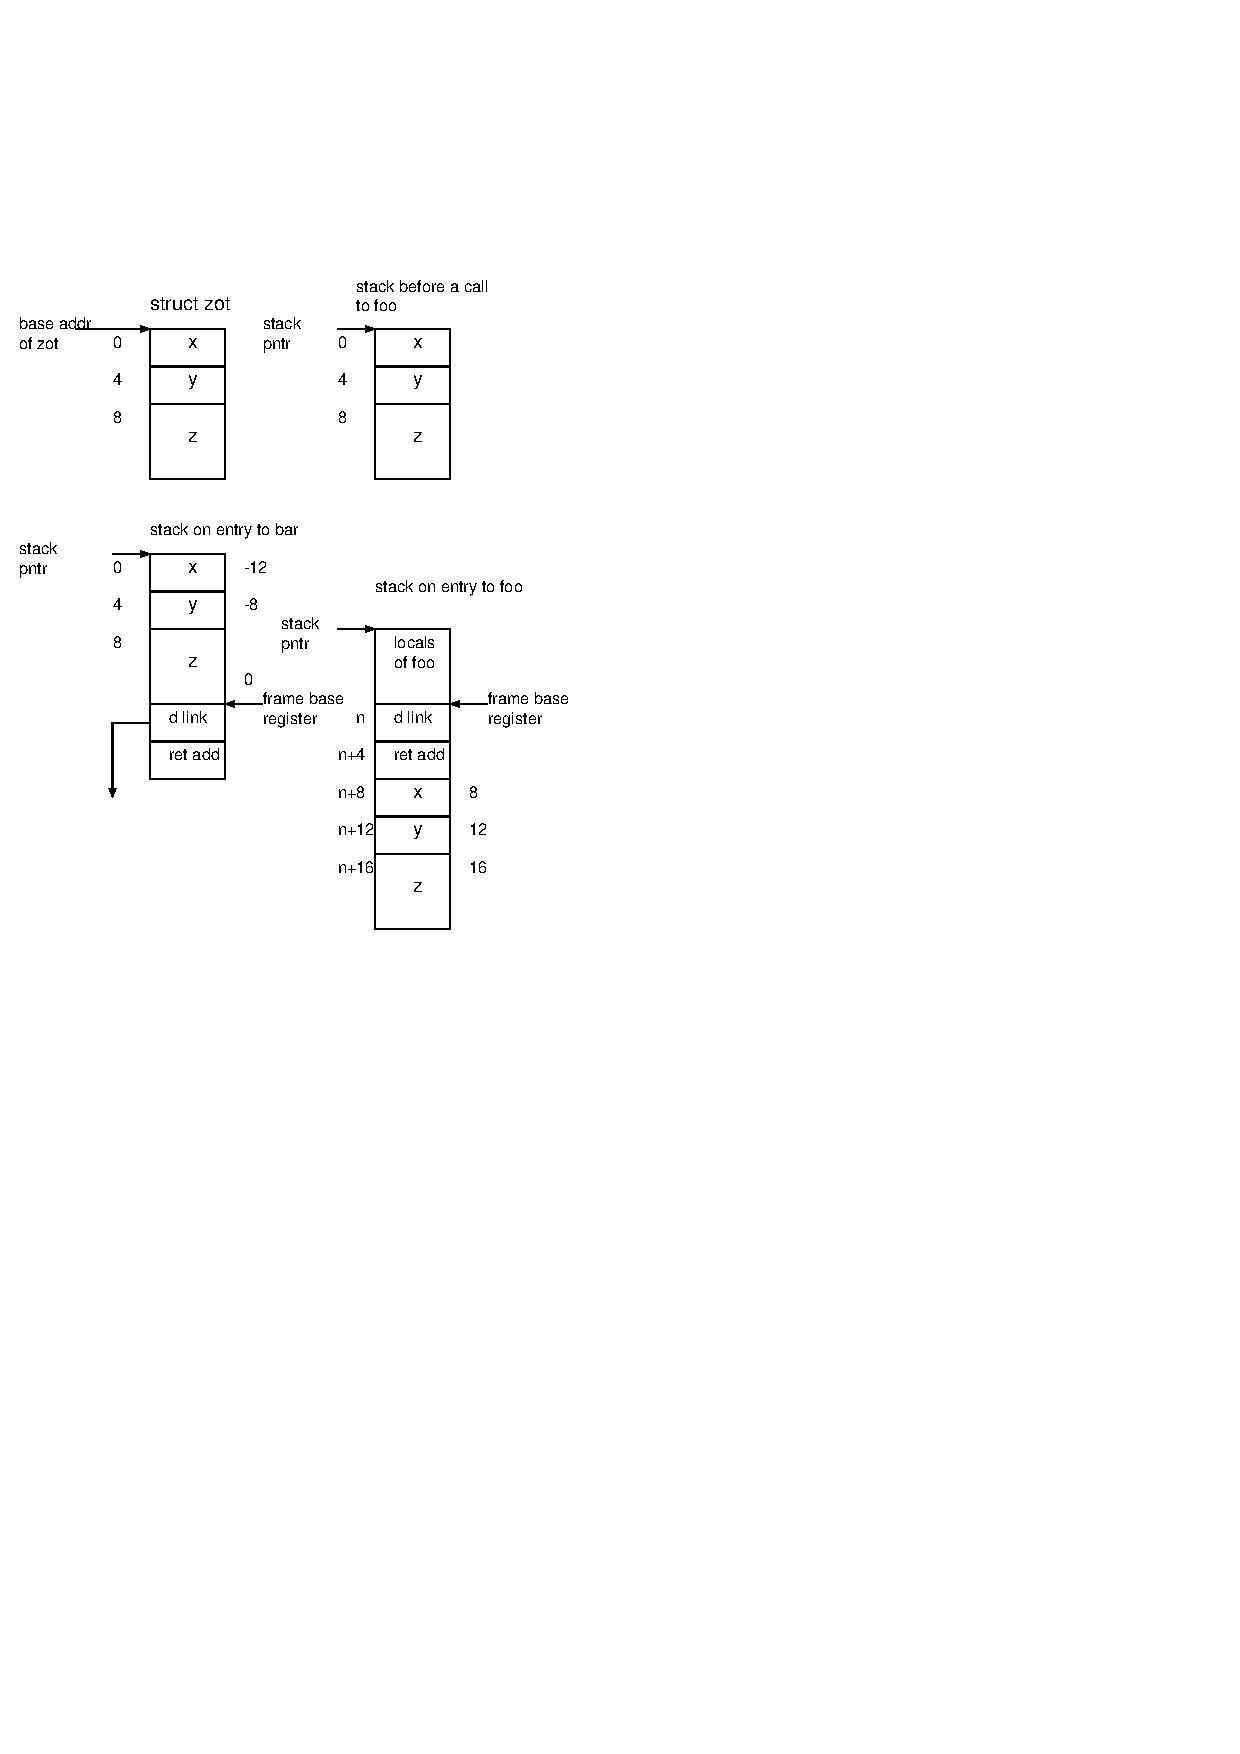
\includegraphics[%
  scale=0.75]{structplusstack.png}\end{center}


\caption{Stacks and records\label{cap:Stacks-and-records}}
\end{figure}

\subsection{Var Params}

We have been assuming value parameters.

If we have var parameters ( parameters which, when assigned to, change
the value of the actual parameter ) then the address of the parameter
rather than the value of the parameter has to be passed on the stack.
The compiler then places and extra level of indirection onto the addressing
of the parameter.


\subsection{Nested Functions}

The existence of nesting of functions and procedures generates
complexities that force us to use a more elaborate calling method than C.
Consider the following Pascal example where we allow function nesting.

\begin{lyxcode}
type~vec1~=~array{[}1..10{]}~of~~integer;

~~~~~~~~scalar~=~integer;

function~sum(var~v:vec1);scalar;



~~function~total(~i:scalar):scalar;

~~begin

~~~~~total:=if~i<1~then~0~else~v{[}i{]}+total(i-1);

~~end

~~total(length(v))



\end{lyxcode}
Total recurses on i, but each invocation accesses the same copy of
v.

Can we use the d-link to access v?

No

Consider the situation below

\includegraphics[%
  scale=0.75]{firstinvocationoftotal.png}

At this point we can access v at mem{[}dlink+8{]}, but what happens
on the next recursion?

\includegraphics[%
  scale=0.75]{secondinvocationoftotal.png}

if we use mem{[}dlink+8{]} we get the previous version of i, v is
now at mem{[}mem{[}dlink{]}+8{]}

We need an alternative approach. There are    3 practical alternatives:

\begin{itemize}
\item Displays
\item Static Links
\item Lambda Lifting
\end{itemize}
We have chosen to use displays since Intel hardware provides support for these.
They do place slight restrictions on function parameters\footnote{ A functions $f$
may not be an actual parameter to procedure or function $g$, if the  scope of $g$
outer to that of $f$}, but it was felt that the simplicity of
display implementation, and the ability to use the same calling
mechanism as C outweighed this.
\subsubsection{Displays }

These can use the Intel Enter instruction defined as:

\begin{lyxcode}
enter~storage,level

~push~ebp

~temp:=esp

~if~level>0

~then~~

~~~~~~repeat~(level-1)~times

~~~~~~~~ebp:=ebp-4

~~~~~~~~push~dword{[}ebp{]}

~~~~~~end~repeat

~~~~~~push~temp

~fi

~ebp:=temp

~esp:=esp~-~storage


\end{lyxcode}
For machines other than the Intel family, you, as a compiler modifier,
have to generate sequences of simpler instructions to emulate the
Intel Enter instruction.

Up to now we have assumed procedures use

\begin{lyxcode}
enter~xxx,0
\end{lyxcode}
Consider the effect of using enter 0,1 for sum and enter 0,2 for total
:

\begin{lyxcode}
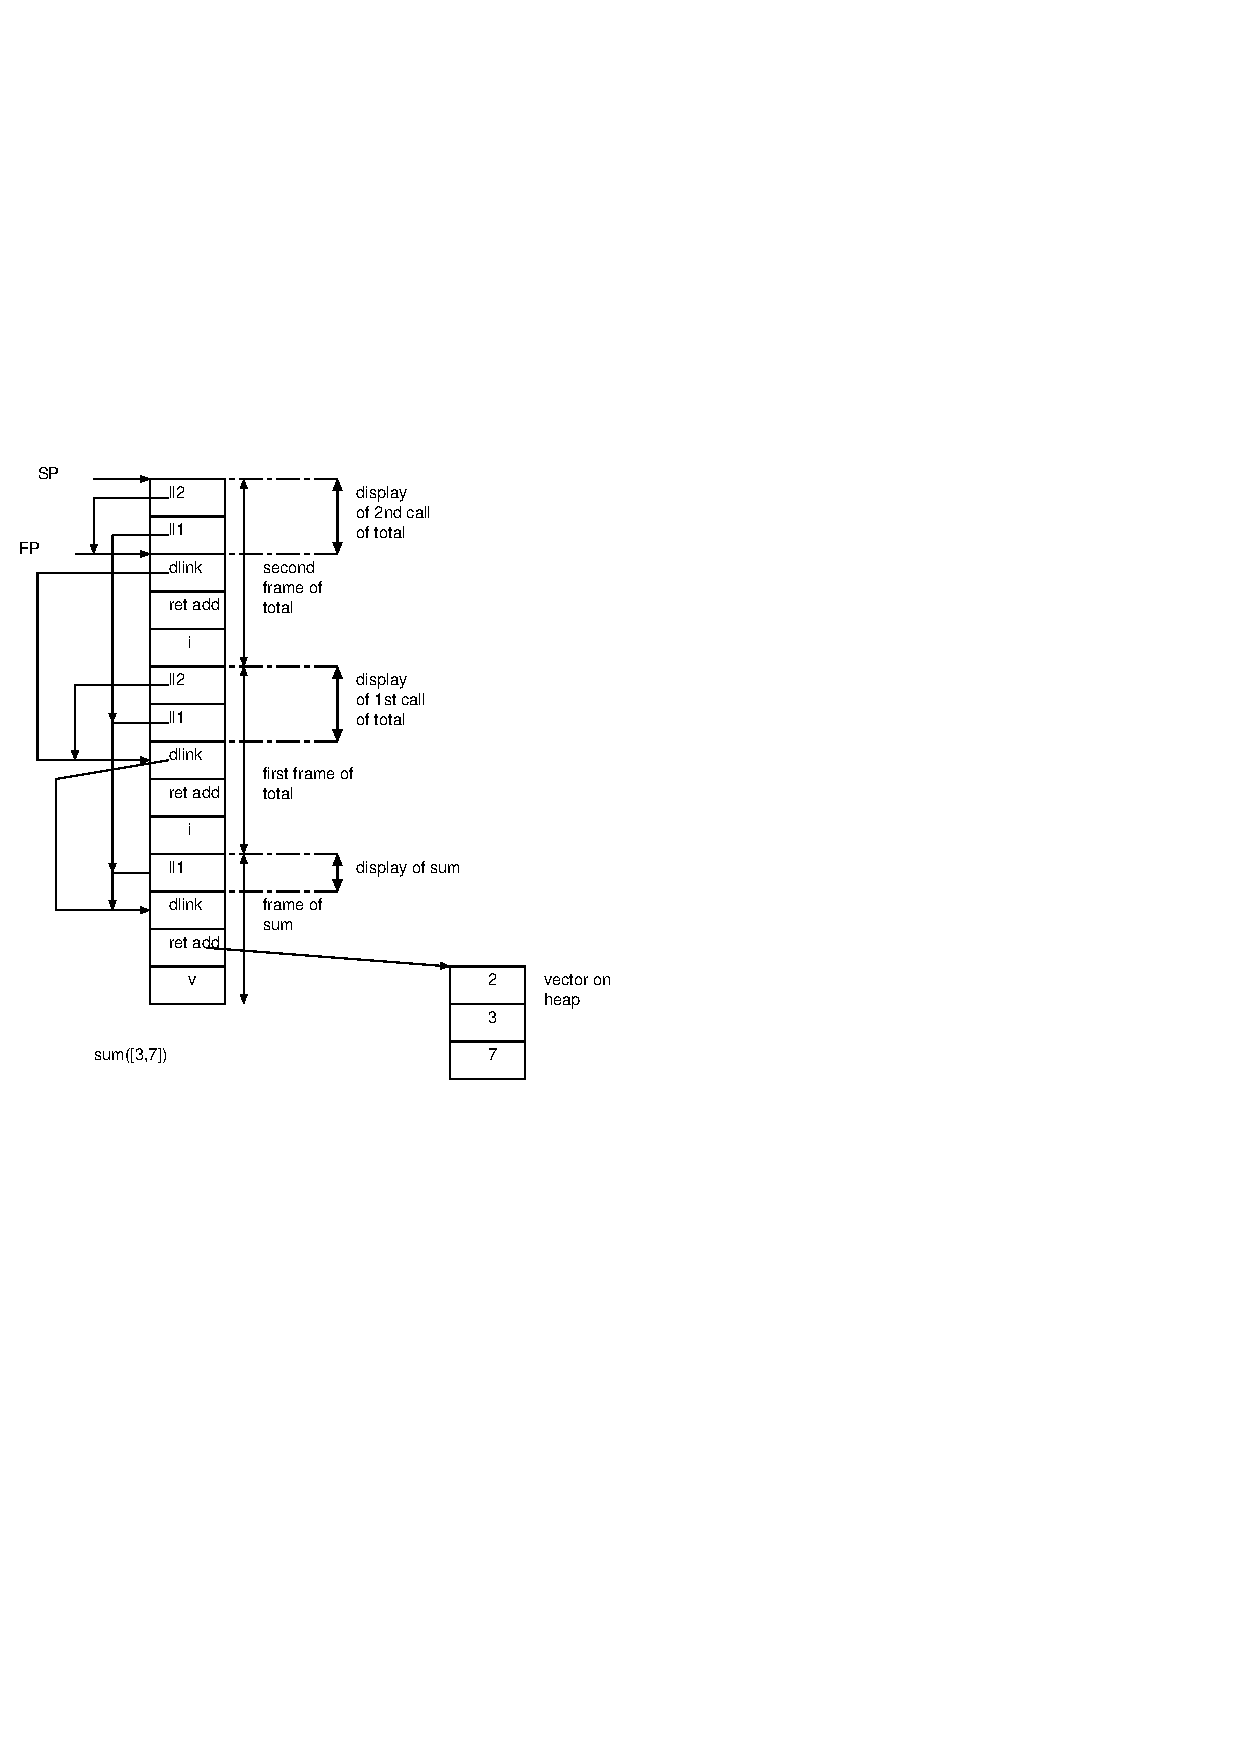
\includegraphics[%
  scale=0.75]{stackwithdisplay.png}
\end{lyxcode}
All variables are now addressed as a pair (lexlevel,offset), where
an outer level function is lexical level 1, the first nested function
is lexical level 2 etc.

A parameter can now be addressed as

\begin{lyxcode}
mem[ display[lexlevel]+offset]

\end{lyxcode}
The display is an array in memory at the start of the current frame.
Using this notation, parameter i is always addressed as

\begin{lyxcode}
mem[display[2]+8]= mem[ mem[fp-8]+8]

\end{lyxcode}
and v is always at

\begin{lyxcode}
mem[display[1]+8]

\end{lyxcode}
hh


\paragraph{Optimisations}

FP always points to the current lexical level so at lexical level
2 we have

\begin{lyxcode}
~~mem{[}display{[}2{]}+8{]}

=~mem{[}~mem{[}fp-8{]}+8{]}

=~mem{[}fp+8{]}
\end{lyxcode}
Likewise we can chose to cache other display values in registers so
avoiding repeated dereferencing of the display on stack.

Other registers sometimes have to be saved because of the definition
of the ABI of the processor. If this is the case then they
are saved after space has been reserved for local variables as
shown in Figure \ref{fullframe}.
\begin{figure}

\includegraphics[%
  scale=0.75]{fullframe.png}
\caption{Full stack frame layout}\label{fullframe}
\end{figure}

\subsection{Detail of calling method used on the Pentium}
Procedure parameters are passed using a modified C calling convention to facilitate
calls to external C procedures. Parameters are pushed on to the stack from right
to left. Value parameters are pushed entire onto the stack, var parameters are
pushed as addresses.


\paragraph{Example }

\begin{verbatim}
program callconv;
type t1= record a,b:integer end;
var
   x,y:t1;
  procedure foo(var a:t1; b:t1; c:integer);
  begin
  end;

  function bar:t1;
  begin bar:=y;end;

begin
        x:=bar;
        foo(x,y,3);
end.
\end{verbatim}
This would generate the following code for the procedure foo.

\begin{verbatim}
; procedure generated by code generator class ilcg.tree.PentiumCG;0
label114b8f429f3a:;0
;    foo;0
; entering a procedure at lexical level 1;0
 enter spaceforfool1-4*1,1;   create display and variable space
   push ebx;             save registers as demanded by Linux ABI
   push esi;
   push edi;
; ------------------          Code for Foo would go here if
;-------------------          it were not a null procedure

spaceforfool1 equ 4;          declare space needed this is done here
                   ;          because the code generation may cause
                   ;          new temporary vars to be needed so
                   ;          we dont know the space required to here
fool1exit:;2
   pop edi;              restore saved registers
   pop esi;0
   pop ebx;0
leave;                        restore old stack frame
 ret 0;                       pop return address into PC
\end{verbatim}
and the calling code is

\begin{verbatim}
 push DWORD      3;                    right most parameter 3
 lea esp,[  esp+     -8];              create space for y on stack
 movq MM4, [   PmainBase+     -16];    fetch y
 movq  [ esp],MM4;                     store on the stack
 push DWORD   PmainBase+     -8;       push the address of x
 EMMS ;                                clear mmx status flags
  call label114b8f429f3a;              call the procedure
 add esp, 16;                          restore the stack

\end{verbatim}

\subsubsection{Function results }

Function results are returned in registers for scalars following the C calling
convention for the operating system on which the compiler is implemented. Records,
strings and sets are returned by the caller passing an implicit parameter containing
the address of a temporary buffer in the calling environment into which the
result can be assigned. Given the following program



The call of {\tt bar} in the previous example would generate

\begin{verbatim}
 push DWORD   PmainBase+     -24;        pass the address of a result buffer
 call label114b8f429f712;                call the function
 add esp, 4;                             restore the stack
 movq MM4, [   PmainBase+     -24];      get the result buffer in MM4
 movq  [   PmainBase+     -8],MM4;       store in x
\end{verbatim}




\section{Multi-core Parallelism}

SIMD vectorisation works for one dimensional\index{vectorise}
 data, or on the last
 dimension for arrays stored in row major order, because the hardware
has to work on adjacent words. SIMD gives considerable acceleration on
 image data, and worthwhile accelerations on floating point and integer
 data. Future machines like the Larrabee will have considerably
wider SIMD registers, increasing the benefits of SIMD code. But newer
chips also have multiple cores. For these, the recent versions of
the Glasgow Pascal Compiler will parallelise across multiple cores\index{parallelise}
if the arrays being worked on are of rank 2. The Pascal source code
of the program remains the same independently of whether it is being
targeted at a simple sequential machine, a SIMD machine or a multi-core
SIMD machine. Targeting is done by flags passed to the compiler:

\begin{lyxcode}
vpc~sub2dex~-cpu486
\end{lyxcode}

would compile sub2dex.pas using purely sequential 32 bit instructions.

\begin{lyxcode}
vpc~sub2dex~-cpuOpteron
\end{lyxcode}

would compile the same file targeted to a 64 bit Opteron with 1 core
using the SIMD instructions in the Opteron instructionset.

\begin{lyxcode}
vpc~sub2dex~-cpuOpteron~-cores2
\end{lyxcode}

would compile the file to a 64 bit Opteron with 2 cores and SIMD instructions.
The compiler is implemented in Java so the selection of code generators
and compilation strategies is achieved by dynamically loading appropriate
compiler and code generator classes.

Let us now look at the transformations required to achieve this using
a trivial rank 2 array example in Algorithm \ref{alg:Example-of-combined}.
The example is not intended to be realistic or useful, only illustrative.
We assume that the code has been compiled for a dual core Opteron.

%
\begin{algorithm}
\caption{Example of combined mult-core and SIMD parallelism.\label{alg:Example-of-combined}}

\begin{lyxcode}
\textcolor{red}{\footnotesize procedure}{\footnotesize{}~sub2d;}{\footnotesize \par}

\textcolor{red}{\footnotesize type}{\footnotesize{}~range=0..127;~}{\footnotesize \par}

\textcolor{red}{\footnotesize var}{\footnotesize{}~x,y,z:}\textcolor{red}{\footnotesize array}{\footnotesize {[}range,range{]}~}\textcolor{red}{\footnotesize of~real}{\footnotesize ;}{\footnotesize \par}

\textcolor{red}{\footnotesize begin}{\footnotesize \par}

{\footnotesize{}~~~~~~~~x:=y-z;}{\footnotesize \par}

\textcolor{red}{\footnotesize end}{\footnotesize ;}{\footnotesize \par}
\end{lyxcode}

This translates into ILCG as follows when compiled for a dual core
Opteron

\begin{lyxcode}
\textcolor{red}{\footnotesize procedure}{\footnotesize (sub2d,}{\footnotesize \par}

{\footnotesize{}~}\textcolor{red}{\footnotesize procedure}{\footnotesize{}~(label12~}\textcolor{green}{\footnotesize ...~see~Algorithm~\ref{alg:The-function-performing}}{\footnotesize{}~)}{\footnotesize \par}

{\footnotesize{}~post\_job{[}label12,\textasciicircum{}(\%rbp),1{]};~~~/{*}~}\textcolor{green}{\footnotesize send~to~core~1}{\footnotesize{}~{*}/}{\footnotesize \par}

{\footnotesize{}~/{*}~Note~that~\%rbp~is~the~Opteron~stack~frame~pointer~{*}/~~~~~~~~~~}{\footnotesize \par}

{\footnotesize{}~post\_job{[}label12,\textasciicircum{}(\%rbp),0{]};~~~/{*}~}\textcolor{green}{\footnotesize send~to~core~0}{\footnotesize{}~{*}/~~~~~~~~~~~~~}{\footnotesize \par}

{\footnotesize{}~wait\_on\_done{[}0{]};}{\footnotesize \par}

{\footnotesize{}~wait\_on\_done{[}1{]};}{\footnotesize \par}

{\footnotesize )}{\footnotesize \par}
\end{lyxcode}

\end{algorithm}


Two threads are dispatched to process the work using a fork - rejoin
paradigm. The run time library is built on top of pthreads\index{pthreads}.
For a two core machine, two server threads\index{thread} are initiated at program
start up. These wait on a semaphore\index{semaphore} until post\_job passes them the
address of a procedure and a stack frame context within which the
procedure is to be executed.

The statement x:=y-z  is translated into a procedure that can run
as a separate task, the ILCG has been simplified for comprehensibility
in Algorithm \ref{alg:The-function-performing}.

%
\begin{algorithm}
\caption{The function performing nested loops.\label{alg:The-function-performing}}

\begin{lyxcode}
\textcolor{red}{\scriptsize procedure}{\scriptsize{}~(label12~/{*}~}\textcolor{green}{\scriptsize internal~label}{\scriptsize {*}/~,}{\scriptsize \par}

{\scriptsize{}~}\textcolor{red}{\scriptsize for}{\scriptsize (mem(+(\textasciicircum{}(\%rbp),-24)),\textasciicircum{}(mem(+(\textasciicircum{}(\%rbp),16))),127~~,~~~}\textbf{\textcolor{blue}{\scriptsize 2}}{\scriptsize ,~}{\scriptsize \par}

{\scriptsize{}~~~~~/{*}}\textcolor{green}{\scriptsize iota~{[}0{]}~~~~~~~~~~~~~task~number~~~~~~~~limit~~step}{\scriptsize {*}/}{\scriptsize \par}

{\scriptsize{}~~}\textcolor{red}{\scriptsize var}{\scriptsize (mem(+(\textasciicircum{}(\%rbp),-32))),/{*}~iota{[}1{]}~{*}/}{\scriptsize \par}

{\scriptsize{}~~}\textcolor{red}{\scriptsize for}{\scriptsize (mem(+(\textasciicircum{}(\%rbp),-32)),~0~~~~,127,~~~~~}\textbf{\textcolor{blue}{\scriptsize 4}}{\scriptsize{}~,}{\scriptsize \par}

{\scriptsize{}~~~~~/{*}}\textcolor{green}{\scriptsize iota~{[}1{]}~~~~~~~~~~~~start~limit~~step}{\scriptsize {*}/}{\scriptsize \par}

{\scriptsize{}~~~mem(ref~ieee32~vector~(~4~),~/{*}~}\textcolor{green}{\scriptsize x{[}iota{[}0{]},iota{[}1{]}{]}}{\scriptsize{}~{*}/}{\scriptsize \par}

{\scriptsize{}~~~~~~~+(+({*}(\textasciicircum{}(mem(+(\textasciicircum{}(\%rbp),-24))),512),~}{\scriptsize \par}

{\scriptsize{}~~~~~~~~~+({*}(\textasciicircum{}(mem(+(\textasciicircum{}(\%rbp),-32))),~~4),-131072)),~}{\scriptsize \par}

{\scriptsize{}~~~~~~~~~~~\textasciicircum{}(mem(+(\textasciicircum{}(\%rbp),-8))))):=}{\scriptsize \par}

{\scriptsize{}~~~~~-(\textasciicircum{}(mem(ref~ieee32~vector~(~4~),/{*}~}\textcolor{green}{\scriptsize y{[}iota{[}0{]},iota{[}1{]}{]}}{\scriptsize{}~{*}/}{\scriptsize \par}

{\scriptsize{}~~~~~~~+(+({*}(\textasciicircum{}(mem(+(\textasciicircum{}(\%rbp),-24))),512),~}{\scriptsize \par}

{\scriptsize{}~~~~~~~~~+({*}(\textasciicircum{}(mem(+(\textasciicircum{}(\%rbp),-32))),~~4),-196608)),~}{\scriptsize \par}

{\scriptsize{}~~~~~~~~~~~\textasciicircum{}(mem(+(\textasciicircum{}(\%rbp),-8)))))),}{\scriptsize \par}

{\scriptsize{}~~~~~~~\textasciicircum{}(mem(ref~ieee32~vector~(~4~),/{*}~}\textcolor{green}{\scriptsize z{[}iota{[}0{]},iota{[}1{]}{]}}{\scriptsize{}~{*}/}{\scriptsize \par}

{\scriptsize{}~~~~~~~~~+(+({*}(\textasciicircum{}(mem(+(\textasciicircum{}(\%rbp),~-24))),512),~}{\scriptsize \par}

{\scriptsize{}~~~~~~~~~~~+({*}(\textasciicircum{}(mem(+(\textasciicircum{}(\%rbp),~-32))),~~4),-262144)),~}{\scriptsize \par}

{\scriptsize{}~~~~~~~~~~~~~\textasciicircum{}(mem(+(\textasciicircum{}(\%rbp),-8))))))))),}{\scriptsize \par}

{\scriptsize{}~)}
\end{lyxcode}

\end{algorithm}

\begin{lyxcode}
{\scriptsize{}~~~~~~}~~~~~~~~~~~~~~~
\end{lyxcode}
The basic structure of the task procedure is two nested for loops,
one for each dimension of the arrays.

The outer loop or row index steps by 2 to ensure that each task will
process every 2nd row, starting at the row given by the task number.
Thus task 0 will process rows 0,2,4,6,... Task 1 will proocess rows
1,3,5,7,... If there are 4 cores available each task will process
every 4th row, etc.

The inner loop, for the column indices, advances by 4 since the Opteron
has SIMD registers capable of handling 4 floating point numbers at
a time.


\subsection{The PURE Function Extension}\index{pure}

We define a pure function to be such that does not have any side effects,
i.e. it does not update any global, or shared, states outside of its
own scope. If the other functions are called from the body of the
function, these also have to be pure even if not marked as such. This
definition of pure functions is consistent with the definition used
in FORTRAN 95. Given the absence of explicit multi-threading constructs
in the given language, the above property of pure functions implies
thread safety. A function can be labeled as pure by prepending the
keyword \texttt{pure} in front of every declaration or definition
of the function. This means that if, for example, a function is declared
as pure in the interface section of the programme, it must be also
declared as pure anywhere else in the code, e.g. in the subsequent
definition of the function body. Any inconsistency in the declared
purity of a function is spotted by the compiler and treated as a syntactic
error.

\begin{lyxcode}
\textbf{pure}~\textbf{function}~next(i~:~integer):~integer;

\textbf{begin}

~~~~~~~~next~:=~i+1;

\textbf{end};
\end{lyxcode}

Above function \emph{next} operates only on the parameter passed to
it, thus it is appropriate to declare it as pure. The keyword \emph{pure}
does not bare any semantic value, other than it serves as a hint to
the compiler which may then generate multi-threaded code. Multi-threaded
code will be generated if -cores\emph{n} flag is passed to the compiler
specifying more than one core, and hence the number of threads, available
to the programme and if the function is then invoked as part of an
assignment statement.


\subsection{Task Parallelism and Block Structure}

The technique of procedurising code shown in Algorithms \ref{alg:Example-of-combined}
and \ref{alg:The-function-performing} is well established when parallelising
loops in Open-MP. There are two significant
differences. First, and least significantly, in Vector Pascal the
loop is implicit rather than the explicit loops used in Open-MP. But
secondly Open-MP is targeted at C and FORTRAN which are flat languages.
Pascal is a block structured language which makes the access to variables
by spawned tasks somewhat more complex. Consider Algorithm \ref{alg:Taylor-series-example.}
which illustrates the use of nested blocks in Pascal. This has a main
program \texttt{nestpar} and embedded within that a procedure \texttt{emap}
which takes a matrix $a$ as a parameter and replaces each $a_{i,j}$
with $e^{scale.a_{i,j}}$ where $scale$ is a global variable. The
exponential function is approximated by a Taylor series

\[
e^{x}=1+\frac{1}{1!}x^{1}+\frac{1}{1!}x^{1}+\frac{1}{2!}x^{2}+\frac{1}{3!}x^{3}+...\]


using the function \texttt{Taylor}. The Taylor series is evaluated
as

{\textsf{\textit{Taylor}$\leftarrow$  $\sum$  (\textit{coefs} $\times$ \textit{x}$^{\iota_{0}}$) }; }

where $\iota_{0}=0,1,2,3...$ using the line

\begin{lyxcode}
Taylor:=~~~\textbackslash{}+~(coefs~{*}~x~pow~iota{[}0{]});
\end{lyxcode}

The coefs vector has been initialised in the main program to contain
the inverse factorial series as required.

%
\begin{algorithm}
\label{alg:Taylor-series-example.}\caption{Taylor series example.}

\begin{lyxcode}
{\footnotesize program~nestpar;}{\footnotesize \par}

{\footnotesize type~t~=~array{[}1..3,1..2{]}~of~real;}{\footnotesize \par}

{\footnotesize{}~~~~~coef=array{[}0..5{]}~of~real;}{\footnotesize \par}

{\footnotesize{}~~~~~~~~~~~~~~~~\{~tabulate~inverse~factorials~\}}{\footnotesize \par}

{\footnotesize const~expc:coef=(1,1,1/2,1/6,1/24,1/(5{*}24));}{\footnotesize \par}

{\footnotesize var~scale:real;B:t;}{\footnotesize \par}

{\footnotesize procedure~emap(var~a:t);}{\footnotesize \par}

{\footnotesize{}~~\{~for~each~a{[}i,j{]}~replace~with~a{[}i,j{]}+exp(scale{*}a{[}i,j{]})~\}}{\footnotesize \par}

{\footnotesize{}~~var~coefs:coef;}{\footnotesize \par}

{\footnotesize{}~~pure~function~Taylor(~x:real):real;}{\footnotesize \par}

{\footnotesize{}~~begin}{\footnotesize \par}

{\footnotesize{}~~~~Taylor:=~~~\textbackslash{}+~(coefs~{*}~x~pow~iota{[}0{]});}{\footnotesize \par}

{\footnotesize{}~~end;}{\footnotesize \par}

{\footnotesize begin}{\footnotesize \par}

{\footnotesize{}~~~coefs:=~expc;}{\footnotesize \par}

{\footnotesize{}~~~a~:=~Taylor(a{*}scale);}{\footnotesize \par}

{\footnotesize end;}{\footnotesize \par}

{\footnotesize begin}{\footnotesize \par}

{\footnotesize{}~~~~~scale:=0.1;}{\footnotesize \par}

{\footnotesize{}~~~~~B:=~iota{[}0{]}{*}iota{[}1{]};}{\footnotesize \par}

{\footnotesize{}~~~~~write(B);}{\footnotesize \par}

{\footnotesize{}~~~~~emap(B);}{\footnotesize \par}

{\footnotesize{}~~~~~write(B);}{\footnotesize \par}

{\footnotesize end.}{\footnotesize \par}
\end{lyxcode}
Output Produced
\begin{lyxcode}
{\footnotesize{}~~~~~1.00000~~~~~2.00000}{\footnotesize \par}

{\footnotesize{}~~~~~2.00000~~~~~4.00000}{\footnotesize \par}

{\footnotesize{}~~~~~3.00000~~~~~6.00000}{\footnotesize \par}

{\footnotesize{}~~~~~~~}{\footnotesize \par}

{\footnotesize{}~~~~~1.10517~~~~~1.22140}{\footnotesize \par}

{\footnotesize{}~~~~~1.22140~~~~~1.49182}{\footnotesize \par}

{\footnotesize{}~~~~~1.34986~~~~~1.82205}
\end{lyxcode}

\end{algorithm}


%
\begin{figure}
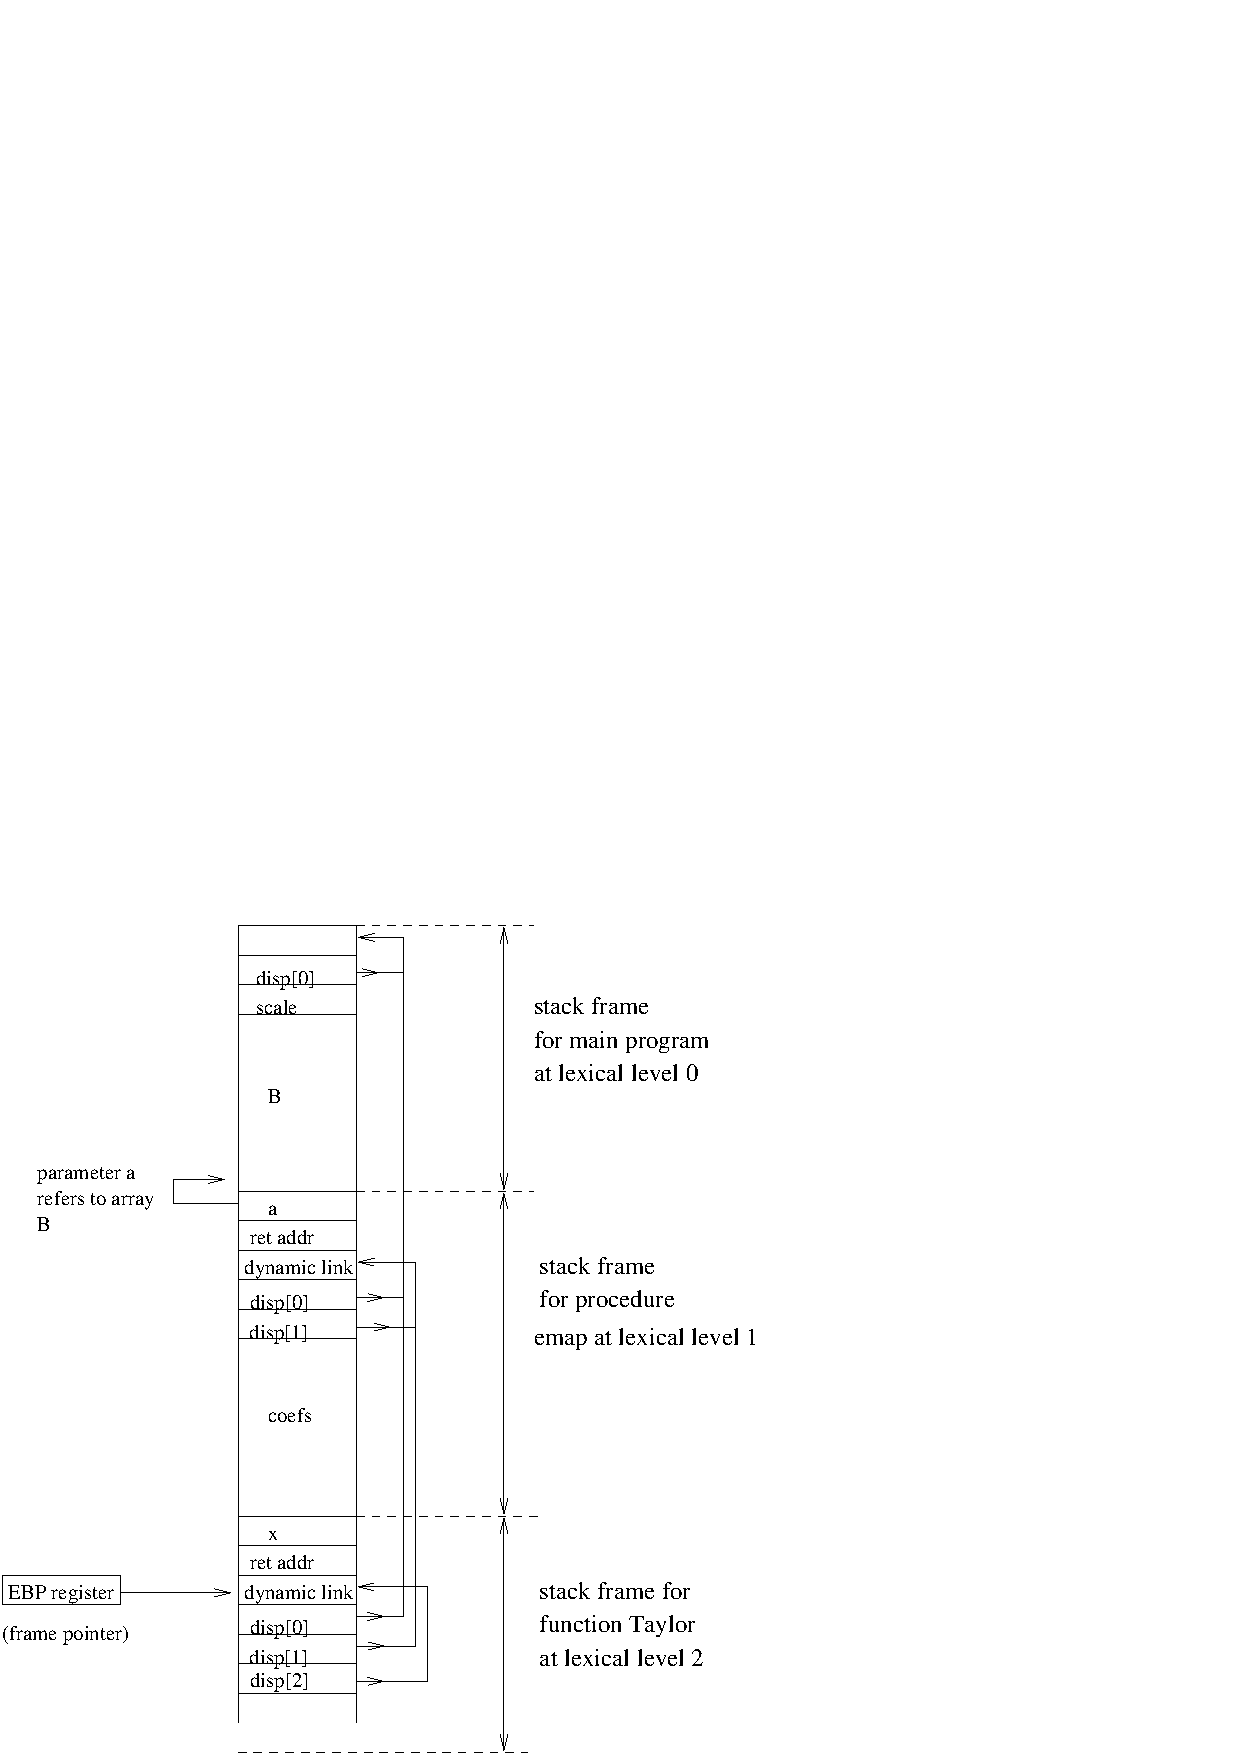
\includegraphics[scale=0.5]{nestparstack1.png}

\caption{Stack for nestpar in single core mode.\label{fig:Stack-for-nestpar}}



\end{figure}


There are a number of references from inner to outer scopes: \texttt{Taylor}
uses the vector \texttt{coefs}, and \texttt{emap} uses the variable
\texttt{scale}. There are three well known techniques for implementing
this in normal procedural code: $\lambda$lifting, static chaining
or display vectors. Since Intel provide direct hardware support for
display vectors in the procedure ENTER and LEAVE instructions we have
chosen to use displays. Figure \ref{fig:Stack-for-nestpar} illustrates
how the stack would be organised during execution of Taylor when the
program is compiled for a single core machine. Observe how Taylor
can access variables in the enclosing stack frames using the display
vector. But if the code is to run on a dual core machine there will
be not one but three stacks as shown in Figure \ref{fig:The-3-stacks}:
one for the main program and one each for the child tasks. The original
function \texttt{emap} will have been written to ILCG equivalent to:

\begin{lyxcode}
{\footnotesize procedure~emap(var~a:t);}{\footnotesize \par}

{\footnotesize{}~~var~coefs:coef;}{\footnotesize \par}

{\footnotesize{}~~pure~function~Taylor(~x:real):real;}{\footnotesize \par}

{\footnotesize{}~~begin}{\footnotesize \par}

{\footnotesize{}~~~~Taylor:=~~~\textbackslash{}+~(coefs~{*}~x~pow~iota{[}0{]});}{\footnotesize \par}

{\footnotesize{}~~end;}{\footnotesize \par}

{\footnotesize{}~~procedure~dummy(start:int);}{\footnotesize \par}

{\footnotesize{}~~var~iota:array{[}0..1{]}~of~integer;}{\footnotesize \par}

{\footnotesize{}~~begin}{\footnotesize \par}

{\footnotesize{}~~~~iota{[}0{]}:=start;}{\footnotesize \par}

{\footnotesize{}~~~~while~iota{[}0{]}<=3~do}{\footnotesize \par}

{\footnotesize{}~~~~begin}{\footnotesize \par}

{\footnotesize{}~~~~~~for~iota{[}1{]}:=1~to~2~do}{\footnotesize \par}

{\footnotesize{}~~~~~~~a{[}iota{[}0{]},iota{[}1{]}{]}:=Taylor(a{[}iota{[}0{]},iota{[}1{]}{]}{*}scale);}{\footnotesize \par}

{\footnotesize{}~~~~~~iota{[}0{]}:=iota{[}0{]}+2;}{\footnotesize \par}

{\footnotesize{}~~~~end;}{\footnotesize \par}

{\footnotesize{}~~end;}{\footnotesize \par}

{\footnotesize begin}{\footnotesize \par}

{\footnotesize{}~~~coefs:=~expc;}{\footnotesize \par}

{\footnotesize{}~~~post\_job(dummy,1);post\_job(dummy,0);}{\footnotesize \par}

{\footnotesize{}~~~wait\_on\_done(0);wait\_on\_done(1);}{\footnotesize \par}

{\footnotesize end;}{\footnotesize \par}
\end{lyxcode}
%

\begin{figure}
\includegraphics[width=14cm]{nestparstack3.png}

\caption{The 3 stacks used by nestpar in dual core mode.\label{fig:The-3-stacks}}



\end{figure}


The function \texttt{dummy} has to run on a task stack and yet have
access to the variable \texttt{a} in \texttt{emap} and \texttt{scale}
in the main program, both of which are executing on the main stack.
It then has to call \texttt{Taylor} in such a way as to ensure that
\texttt{Taylor} can access the global \texttt{scale}. Provided that
the displays can be set up as shown in Figure \ref{fig:The-3-stacks},
this will work, but it is impossible to set up the displays this way
when using standard intel call conventions along with the \texttt{pthreads}
library. Whenever a function is executed within a thread it is allocated
a new stack that does not contain display pointers, hence variables
from containing scopes cannot be accessed.

In order to support sharing of the global stack amongst multiple tasks,
we have implemented an assembly routine \emph{taskexecute}, which
corresponds to the following C function signature:

\begin{lyxcode}
void~taskexecute(struct~threadblock~{*});
\end{lyxcode}

As can be seen, the function expects a single parameter which is a
pointer to a structure of type \emph{struct threadblock} defined as

\begin{lyxcode}
struct~threadblock\{
\begin{lyxcode}

char~{*}~savedframepointer;

char~{*}~savedcodepointer;

int~threadnumber;

\end{lyxcode}
\}
\end{lyxcode}

Above, \texttt{savedframerpointer} is the pointer to the original
stack in which the displays are already setup, \texttt{savedcodepointer}
is the pointer to the function that is being parallelised, and \texttt{threadnumber}
is a number in the range$0..n-1$ for a programme running on$n$ cores..
The following assembly code implements \texttt{taskexecute} on the
Pentium architecture.

\emph{Assembly code sequence required to implement the task execute}

\begin{lyxcode}
{\footnotesize .globl~taskexecute}{\footnotesize \par}

{\footnotesize taskexecute:}{\footnotesize \par}

{\footnotesize \#~on~entry~we~have~a~pointer~in~\%esp~to~the~task~block}{\footnotesize \par}

{\footnotesize \#~this~task~block~has~the~C~definition}{\footnotesize \par}

{\footnotesize \#~struct~threadblock\{}{\footnotesize \par}

{\footnotesize \#~~~~~~~~~char~{*}~savedframepointer;}{\footnotesize \par}

{\footnotesize \#~~~~~~~~~char~{*}~savedcodepointer;}{\footnotesize \par}

{\footnotesize \#~~~~~~~~~int~threadnumber;\}}{\footnotesize \par}

{\footnotesize \#~the~first~thing~we~do~is~save~the~framepointer~on~entry}{\footnotesize \par}

{\footnotesize push~\%ebp}{\footnotesize \par}

{\footnotesize \#~next~get~the~address~of~the~stored~frame~pointer~in~the~task~block}{\footnotesize \par}

{\footnotesize mov~8(\%esp)~,~\%eax}{\footnotesize \par}

\#we~load~the~frame~pointer~into~the~hardware~frame~pointer~(ebp)

{\footnotesize mov~0(\%eax),~\%ebp}{\footnotesize \par}

{\footnotesize \#~get~the~task~number}{\footnotesize \par}

{\footnotesize push~8(\%eax)~}{\footnotesize \par}

{\footnotesize \#~make~the~call~on~the~task}{\footnotesize \par}

{\footnotesize call~{*}~4(\%eax)~}{\footnotesize \par}

{\footnotesize \#~unwind~stack~pointer}{\footnotesize \par}

{\footnotesize add~\$4,\%esp}{\footnotesize \par}

{\footnotesize \#~restore~framepointer~we~were~called~with}{\footnotesize \par}

{\footnotesize pop~\%ebp}{\footnotesize \par}

{\footnotesize ret}{\footnotesize \par}


\end{lyxcode}

The essence of this form of implementation is that the pthread is
setup to execute \texttt{taskexecute} which is passed \texttt{threadblock}
from the calling environment that contains the stack pointer used
by the calling environment. \texttt{taskexecute} substitutes the stack
allocated by the pthread library with the above stack before executing
the code sequence contained in the \texttt{savedcodepointe}\emph{r.}
The effect of substituting the stack pointer is undone once the called
code sequence halts to ensure a clean exit of the wrapper.


\section{Example Programs}


\subsection{Image convolution}

The first example we will look at is the use of a seperable convolution
kernel to blur an image. Convolution of an image by a matrix of real
numbers can be used to smooth or sharpen an image, depending on the
matrix used. If $A$ is an output image, $K$ a convolution matrix,
then if $B$ is the convolved image \[
B_{y,x}=\sum_{i}\sum_{j}A_{y+i,x+j}K_{i,j}\]


A separable convolution kernel is a vector of real numbers that can
be applied independently to the rows and columns of an image to provide
filtering. It is a specialisation of the more general convolution
matrix, but is algorithmically more efficient to implement. We can
do a seperable convolution provided that the kernel is formed by the
outer product of two vectors \textbf{a},\textbf{b}. A symmetric separable
convolution can be done if $\mathbf{a}=\mathbf{b}$.

If \textbf{k} is a symmetric separable convolution vector, then the
corresponding matrix $K$ is such that $K_{i,j}={\bf k}_{i}{\bf k}_{j}$.

Given a starting image $A$ as a two dimensional array of pixels,
and a three element kernel $c_{1},c_{2},c_{3}$, the algorithm first
forms a temporary array $T$ whose whose elements are the weighted
sum of adjacent rows $T_{y,x}=c_{1}A_{y-1,x}+c_{2}A_{y,x}+c_{3}A_{y+1,x}$.
Then in a second phase it sets the original image to be the weighted
sum of the columns of the temporary array: $A_{y,x}=c_{1}T_{y,x-1}+c_{2}T_{y,x}+c_{3}T{y,x+1}$.

Clearly the outer edges of the image are a special case, since the
convolution is defined over the neighbours of the pixel, and the pixels
along the boundaries a missing one neighbour. A number of solutions
are available for this, but for simplicity we will perform only vertical
convolutions on the left and right edges and horizontal convolutions
on the top and bottom lines of the image. A Vector Pascal routine
to do this is given below. The source has been pretty printed in the
latex format that is automatically generated by the compiler is listing
enabled. An equivalent sequential C routine is given in Algorithm
\ref{alg:C-version-of}.

In comparing the C and Vector Pascal, note two features which give
performance advantages to the Vector Pascal form of the algorithm.
\begin{enumerate}
\item The support for fixed point 8 bit arithmetic with the pixel type.
This allows a higher level of parallelism to be achieved since a P4
or AMD64 can in principle operate on 16 $\times$8 bit numbers with
a single instruction. Lacking these types, the C algorithm has to
use 32 bit floats. The pixel type automatically uses saturated arithmetic.
\item The data parallel form of expression of the Vector Pascal allows more
efficient optimisation of the code.
\end{enumerate}

\subsubsection{Vector Pascal convolution algorithm}

\begin{tabbing} {*}{*}{*}\={*}{*}{*}\={*}{*}{*}\={*}{*}{*}\={*}{*}{*}\={*}{*}{*}\={*}{*}{*}\={*}{*}{*}\={*}{*}{*}\={*}{*}{*}\={*}{*}{*}\={*}{*}{*}\={*}{*}{*}\=\kill
\\
 \+%
\parbox[c]{14cm}{%
\textsf{\textbf{type}} %
}\\
 %
\parbox[c]{14cm}{%
plane(rows,cols:\textsf{\textit{integer}} \textsf{)=}\textbf{ array}
\textsf{{[}0..}\textsf{\textit{rows}} \textsf{,0..}\textsf{\textit{cols}}
\textsf{{]}}\textbf{ of} \textsf{\textit{pixel}} \textsf{;}%
}\\
 \<%
\parbox[c]{14cm}{%
\textsf{\textbf{var}} %
}\\
 %
\parbox[c]{14cm}{%
\textsf{Let} \textsf{\textit{T}}\textsf{,} \textsf{\textit{l}} \textsf{$\in$\^{ }plane;}%
}\\
 %
\parbox[c]{14cm}{%
\textsf{Let} \textsf{\textit{i}} \textsf{$\in$ integer;}%
}\\
%
\parbox[c]{14cm}{%
\textsf{\textbf{begin}} %
}\\
 \end{tabbing} Allocates a temporary buffer to hold a plane, and
3 temporary buffers to hold the convolution co-ordinates as lines
of pixels. \begin{tabbing} {*}{*}{*}\={*}{*}{*}\={*}{*}{*}\={*}{*}{*}\={*}{*}{*}\={*}{*}{*}\={*}{*}{*}\={*}{*}{*}\={*}{*}{*}\={*}{*}{*}\={*}{*}{*}\={*}{*}{*}\={*}{*}{*}\=\kill
\+ \\
 %
\parbox[c]{14cm}{%
\textsf{\textbf{new}} \textsf{\textit{(}} \textsf{\textit{T}} \textsf{,}\textsf{\textit{im}}
\textsf{.}\textsf{\textit{maxrow}} \textsf{,}\textsf{\textit{im}}
\textsf{.}\textsf{\textit{maxcol}} \textsf{);}%
}\\
 %
\parbox[c]{14cm}{%
\textsf{\textbf{new}} \textsf{\textit{(}} \textsf{\textit{l}} \textsf{,3,}\textsf{\textit{im}}
\textsf{.}\textsf{\textit{maxcol}} \textsf{);}%
}\\
 %
\parbox[c]{14cm}{%
\textsf{\textit{l}}\textsf{$\uparrow${[}0{]}$\leftarrow$} \textsf{\textit{c1}}; %
}\\
 %
\parbox[c]{14cm}{%
\textsf{\textit{l}}\textsf{$\uparrow${[}1{]}$\leftarrow$} \textsf{\textit{c2}}; %
}\\
%
\parbox[c]{14cm}{%
\textsf{\textit{l}}\textsf{$\uparrow${[}2{]}$\leftarrow$} \textsf{\textit{c3}}; %
}\\
 \end{tabbing} Perform convolution on each of the planes of the
image. This has to be done with an explicit loop as array maps only
works with functions not with procedures. \begin{tabbing} {*}{*}{*}\={*}{*}{*}\={*}{*}{*}\={*}{*}{*}\={*}{*}{*}\={*}{*}{*}\={*}{*}{*}\={*}{*}{*}\={*}{*}{*}\={*}{*}{*}\={*}{*}{*}\={*}{*}{*}\={*}{*}{*}\=\kill
\+ \\
 %
\parbox[c]{14cm}{%
\textsf{\textbf{for}} \textsf{\textit{i}}\textsf{$\leftarrow$ 0}
\textsf{\textbf{to}} \textsf{\textit{im.maxplane}} \textsf{\textbf{do}}
\textsf{\textit{convpar}} \textsf{(}\textsf{\textit{im}}\textsf{$_{\textit{i}}$,}
\textsf{\textit{l}}\textsf{$\uparrow$,} \textsf{\textit{T}}\textsf{$\uparrow$);}
\{ see section \ref{sub:convpar}\}%
}\\
 \end{tabbing} This sequence frees the temporary buffers used
in the convolution process. \begin{tabbing} {*}{*}{*}\={*}{*}{*}\={*}{*}{*}\={*}{*}{*}\={*}{*}{*}\={*}{*}{*}\={*}{*}{*}\={*}{*}{*}\={*}{*}{*}\={*}{*}{*}\={*}{*}{*}\={*}{*}{*}\={*}{*}{*}\=\kill
\+ \\
 %
\parbox[c]{14cm}{%
\textsf{\textbf{dispose}} \textsf{\textit{(}} \textsf{\textit{l}}
\textsf{);}%
}\\
 %
\parbox[c]{14cm}{%
\textsf{\textbf{dispose}} \textsf{\textit{(}} \textsf{\textit{T}}
\textsf{);}%
}\\
 \<\-%
\parbox[c]{14cm}{%
\textsf{\textbf{end}} \textsf{;}%
}\\
 \end{tabbing}


\subsubsection{convpar\label{sub:convpar}}

\label{sec:blurtime/pconvpconvpar}

\begin{tabbing} {*}{*}{*}\={*}{*}{*}\={*}{*}{*}\={*}{*}{*}\={*}{*}{*}\={*}{*}{*}\={*}{*}{*}\={*}{*}{*}\={*}{*}{*}\={*}{*}{*}\={*}{*}{*}\={*}{*}{*}\={*}{*}{*}\=\kill
%
\parbox[c]{14cm}{%
\textsf{\textbf{procedure}} \textsf{\textit{convpar}} \textsf{\textit{(}}
\textsf{\textbf{var}} \textsf{\textit{p}} \textsf{,}\textsf{\textit{l}}
\textsf{,}\textsf{\textit{T}} \textsf{:}\textsf{\textit{plane}} \textsf{);}%
}\\
 \end{tabbing} This convolves a plane by applying the vertical
and horizontal convolutions in turn. \begin{tabbing} {*}{*}{*}\={*}{*}{*}\={*}{*}{*}\={*}{*}{*}\={*}{*}{*}\={*}{*}{*}\={*}{*}{*}\={*}{*}{*}\={*}{*}{*}\={*}{*}{*}\={*}{*}{*}\={*}{*}{*}\={*}{*}{*}\=\kill
\\
 \+%
\parbox[c]{14cm}{%
\textsf{\textbf{var}} %
}\\
 %
\parbox[c]{14cm}{%
\textsf{Let} \textsf{\textit{r}}\textsf{,} \textsf{\textit{c}} \textsf{$\in$
integer;}%
}\\
 \-\<\+%
\parbox[c]{14cm}{%
\textsf{\textbf{begin}} %
}\\
 \end{tabbing} This sequence performs a vertical convolution of
the rows of the plane p and places the result in the temporary plane
$T$. It uses the lines of pixels \textsf{l{[}i{]}} as convolution
weights. Use of lines of pixels rather than the floating point numbers
for the kernel weights allows the computation to proceed 8 pixels
at a time in parallel. The lines \textsf{\textit{T}}\textsf{$_{0}$$\leftarrow$}
\textsf{\textit{p}}\textsf{$_{0}$}; and \textsf{\textit{T}}\textsf{$_{\textit{r}}$$\leftarrow$}
\textsf{\textit{p}}\textsf{$_{\textit{r}}$}; deal with the top and
bottom rows of the picture which are left unchanged.

\begin{tabbing} {*}{*}{*}\={*}{*}{*}\={*}{*}{*}\={*}{*}{*}\={*}{*}{*}\={*}{*}{*}\={*}{*}{*}\={*}{*}{*}\={*}{*}{*}\={*}{*}{*}\={*}{*}{*}\={*}{*}{*}\={*}{*}{*}\=\kill
\+ \\
 %
\parbox[c]{14cm}{%
\texttt{\small {\{\$r-\}\{disable range checks\}}}%
}\\
 %
\parbox[c]{14cm}{%
\textsf{\textit{r}}\textsf{$\leftarrow$} \textsf{\textit{p.rows}}; %
}\\
 %
\parbox[c]{14cm}{%
\textsf{\textit{T}}\textsf{$_{1..\textit{r}-1}$$\leftarrow$} \textsf{\textit{p}}\textsf{$_{0..\textit{r}-2}$
$\times$} \textsf{\textit{l}}\textsf{$_{0}$ +} \textsf{\textit{p}}\textsf{$_{1..\textit{r}-1}$
$\times$} \textsf{\textit{l}}\textsf{$_{1}$ +} \textsf{\textit{p}}\textsf{$_{2..\textit{r}}$
$\times$} \textsf{\textit{l}}\textsf{$_{2}$}; %
}\\
 %
\parbox[c]{14cm}{%
\textsf{\textit{T}}\textsf{$_{0}$$\leftarrow$} \textsf{\textit{p}}\textsf{$_{0}$}; %
}\\
 %
\parbox[c]{14cm}{%
\textsf{\textit{T}}\textsf{$_{\textit{r}}$$\leftarrow$} \textsf{\textit{p}}\textsf{$_{\textit{r}}$}; %
}\\
 \end{tabbing} Now perform a horizontal convolution of the plane
$T$ and place the result in p. \begin{tabbing} {*}{*}{*}\={*}{*}{*}\={*}{*}{*}\={*}{*}{*}\={*}{*}{*}\={*}{*}{*}\={*}{*}{*}\={*}{*}{*}\={*}{*}{*}\={*}{*}{*}\={*}{*}{*}\={*}{*}{*}\={*}{*}{*}\=\kill
\+ \\
 %
\parbox[c]{14cm}{%
\textsf{\textit{c}}\textsf{$\leftarrow$} \textsf{\textit{p.cols}}; %
}\\
 %
\parbox[c]{14cm}{%
\textsf{\textit{p}}\textsf{$_{0..\textit{r},1..\textit{c}-1}$$\leftarrow$}
\textsf{\textit{T}}\textsf{$_{0..\textit{r},0..\textit{c}-2}$ $\times$}
\textsf{\textit{l}}\textsf{$_{0}$ +} \textsf{\textit{T}}\textsf{$_{0..\textit{r},2..\textit{c}}$
$\times$} \textsf{\textit{l}}\textsf{$_{2}$ +} \textsf{\textit{T}}\textsf{$_{0..\textit{r},1..\textit{c}-1}$
$\times$} \textsf{\textit{l}}\textsf{$_{1}$}; %
}\\
 %
\parbox[c]{14cm}{%
\textsf{\textit{p}}\textsf{$_{0..\textit{r},0}$$\leftarrow$} \textsf{\textit{T}}\textsf{$_{0..\textit{r},0}$}; %
}\\
 %
\parbox[c]{14cm}{%
\textsf{\textit{p}}\textsf{$_{0..\textit{r},\textit{c}}$$\leftarrow$}
\textsf{\textit{T}}\textsf{$_{0..\textit{r},\textit{c}}$}; %
}\\
 %
\parbox[c]{14cm}{%
\texttt{\small {\{\$r+\}\{enable range checks\}}}%
}\\
 \\
 \<\-%
\parbox[c]{14cm}{%
\textsf{\textbf{end}} \textsf{;}%
}\\
 \end{tabbing}

%
\begin{algorithm}


\caption{C version of the convolution routine.\label{alg:C-version-of}}

\begin{lyxcode}
\#include~<stdlib.h>

conv(char~{*}im,~int~planes,~int~rows,int~cols,float~c1,float~c2,float~c3)

/{*}~C~version~of~a~convolution~routine~{*}/

\{~

~int~i,j,p,temp;

~int~planestep=rows{*}cols;

~char~{*}~plane,~{*}~buffplane;

~char~{*}~buff~=~malloc(~rows{*}planes{*}cols);

~for~(p=0;p<planes;p++)\{

~~plane~=~\&im{[}p{*}planestep{]};

~~buffplane=~\&buff{[}p{*}planestep{]};

~~/{*}~convolve~horizontally~{*}/

~~for(i=0;i<rows;i++)\{

~~~for(j=1;j<(cols-1);j++)~\{

~~~~temp=~plane{[}i{*}cols+j-1{]}{*}c1+plane{[}i{*}cols+j{]}{*}c2+plane{[}i{*}cols+j+1{]}{*}c3;

~~~~if~(temp<0)\{temp=0;\}

~~~~else~if~(temp>255)~\{~temp=255;\}~;

~~~~buffplane{[}i{*}cols+j{]}=temp;

~~~\}

~~~buffplane{[}i{*}cols{]}=plane{[}i{*}cols{]};

~~~buffplane{[}i{*}cols+cols-1{]}=plane{[}i{*}cols+cols-1{]};

~~\}

/{*}~convolve~vertically~{*}/

~~for(j=0;j<cols;j++)~\{

~~~for(i=1;i<rows-1;i++)\{

~~~~temp=~buffplane{[}(i-1){*}cols+j{]}{*}c1+buffplane{[}i{*}cols+j{]}{*}c2+buffplane{[}(1+i){*}cols+j{]}{*}c3;

~~~~if(temp<0)\{temp=0;\}

~~~~else~if~(temp>255)~\{~temp=255;\}~;

~~~~plane{[}i{*}cols+j{]}=temp;

~~~\}

~~~plane{[}j{]}=buffplane{[}j{]};

~~~plane{[}(rows-1){*}cols+j{]}=buffplane{[}~(rows-1){*}cols+j{]};

~~\}

~\}

~free(buff);

\}
\end{lyxcode}

\end{algorithm}

\section{Array representation}

The maximum number of array dimensions supported in the compiler is 5.

A static\index{static} array\index{array, static} is represented simply by
the number of bytes required to store the array being allocated in the global
segment or on the stack.

A dynamic array\index{array}\index{array, dynamic} is always represented on
the heap\index{heap}. Since its rank\index{rank} is known to the compiler
what needs to be stored at run time are the bounds and the means to access it.
For simplicity we make the format of dynamic and conformant arrays the same.
Thus for schema\index{schema}

\texttt{s(a,b,c,d:integer)= array{[}a..b,c..d{]} of integer }

whose run time bounds are evaluated to be 2..4,3..7 we would have the following
structure:

\vspace{0.2cm}
{\centering \begin{tabular}{|c|c|c|}
\hline
address&
field&
value\\
\hline
\hline
x&
base of data&
address of first integer in the array\\
\hline
x+4&
a&
2\\
\hline
x+8&
b&
4\\
\hline
x+12&
step&
20\\
\hline
x+16&
c&
3\\
\hline
x+20&
d&
7\\
\hline
\end{tabular}\par}
\vspace{0.3cm}

The base address for a schematic array on the heap, will point at the first
byte after the array header shown. For a conformant array, it will point at the
first data byte of the array or array range\index{range} being passed as a
parameter. The step field specifies the length of an element of the second dimension
in bytes. It is included to allow for the case where we have a conformant\index{conformant}
array\index{array, conformant} formal parameter

\texttt{x:array{[}a..b:integer,c..d:integer{]} of integer}

to which we pass as actual parameter\index{parameter} the range

\texttt{p{[}2..4,3..7{]} }

as actual parameter, where \texttt{p:array{[}1..10,1..10{]} of integer}

In this case the base address would point at @p{[}2,3{]} and the step would
be 40 - the length of 10 integers.


\subsection{Range\index{range} checking}\label{rangecheck}

When arrays are indexed, the compiler plants run time checks to see if the indices
are within bounds\index{bounds}. In many cases the optimiser is able to remove
these checks, but in those cases where it is unable to do so, some performance
degradation can occur. Range checks can be disabled or enabled by the compiler
directives.

\{\$r-\} \{ disable range checks \}

\{\$r+\} \{ enable range checks \}

Performance can be further enhanced by the practice of declaring arrays to have
lower bounds of zero. The optimiser is generally able to generate more efficient
code for zero based arrays.



%\chapter{Compiler porting tools}
%\label{ilcg}
%\input ilcg


%\part{VIPER\\\ \\ {\normalsize\em Ken Renfrew}}

%\input viper


\printindex{}

\begin{thebibliography}{10}


\bibitem{ThreeL}
3L Limited, Parallel C V2.2, Software Product Description, 1995.


\bibitem{AMD}Advanced Micro Devices, 3DNow! Technology Manual, 1999.
\bibitem{2}Aho, A.V., Ganapathi, M, TJiang S.W.K., Code Generation Using Tree Matching
and Dynamic Programming, ACM Trans, Programming Languages and Systems 11, no.4,
1989, pp.491-516.



\bibitem{blelloch}
Blelloch, G. E., {\sc Nesl}: A Nested Data-Parallel Language, Carnegie
Mellon University, CMU-CS-95-170, Sept 1995.



\bibitem{Burke}Burke, Chris, J User Manual, ISI, 1995.
\bibitem{Cattel80}Cattell R. G. G., Automatic derivation of code generators from machine descriptions,
ACM Transactions on Programming Languages and Systems, 2(2), pp. 173-190, April
1980.
\bibitem{Chaitin}Chaitin. G., Elegant Lisp Programs, in The Limits of Mathematics, pp. 29-56,
Springer, 1997.
\bibitem{Cheong97}Cheong, G., and Lam, M., An Optimizer for Multimedia Instruction Sets, 2nd SUIF
Workshop, Stanford University, August 1997.
\bibitem{Cherry} Cherry, G., W., Pascal Programming Structures, Reston Publishing, Reston, 1980.
\bibitem{Cockshott00}Cockshott, Paul, Direct Compilation of High Level Languages for Multi-media
Instruction-sets, Department of Computer Science, University of Glasgow, Nov
2000.



\bibitem{Ewing}
Ewing, A. K., Richardson, H., Simpson, A. D., Kulkarni, R., Writing Data
Parallel Programs with High Performance Fortran, Edinburgh Parallel Computing
Centre, Ver 1.3.1.

\bibitem{formella1992spark} Formella, A.; Obe, A.; Paul, W.; Rauber, T. \& Schmidt, D. The SPARK 2.0 system-a special purpose vector processor with a VectorPASCAL compiler System Sciences, 1992. Proceedings of the Twenty-Fifth Hawaii International Conference on, 1992, 1, 547-558.



\bibitem{graham80}Susan L. Graham, Table Driven Code Generation, IEEE Computer, Vol 13, No. 8,
August 1980, pp 25..37.
\bibitem{IA32}Intel, Intel Architecture Software Developers Manual Volumes 1 and 2, 1999.
\bibitem{Intel00}Intel, Willamette Processor Software Developer's Guide, February, 2000.
\bibitem{ISO90}ISO, Extended Pascal ISO 10206:1990, 1991.
\bibitem{ISO90a}ISO, Pascal, ISO 7185:1990, 1991.

\bibitem{Iverson62}K. E. Iverson, A Programming Language, John Wiley \& Sons, Inc., New York (1962),
p. 16.
\bibitem{Iverson80}Iverson, K. E. . Notation as a tool of thought. Communications of the ACM, 23(8),
444-465, 1980.
\bibitem{Jmanual}Iverson K. E, A personal View of APL, IBM Systems Journal, Vol 30, No 4, 1991.
\bibitem{Jintro}Iverson, Kenneth E., J Introduction and Dictionary, Iverson Software Inc. (ISI),
Toronto, Ontario, 1995. 4, pp 347-361, 2000.
\bibitem{Jensen}Jensen, K., Wirth, N., PASCAL User Manual and Report, Springer 1978.

\bibitem{Johnston}
Johnston, D., C++ Parallel Systems, ECH: Engineering Computing Newsletter,
No. 55, Daresbury Laboratory/Rutherford Appleton Laboratory, March 1995,pp 6-7.
\bibitem{Knuth} Knuth, D., Computers and Typesetting, Addison Wesley, 1994.
\bibitem{Krall00}
Krall, A., and Lelait, S., Compilation Techniques for Multimedia Processors,
International Journal of Parallel Programming, Vol. 28, No. 4, pp 347-361, 2000.

\bibitem{Lamport} Lamport, L., \LaTeX a document preparation system, Addison Wesley, 1994.

\bibitem{Leupers99}Leupers, R., Compiler Optimization for Media Processors, EMMSEC 99/Sweden 1999.




\bibitem{Metcalf96}Metcalf, M., and Reid., J., The F Programming Language, OUP, 1996.
\bibitem{Peleg97}Peleg, A., Wilke S., Weiser U., Intel MMX for Multimedia PCs, Comm. ACM, vol
40, no. 1 1997.

\bibitem{Shannon}
Shannon, C., A Mathematical Theory of Communication, The Bell System Technical
Journal, Vol 27, pp 379-423 and 623-656, 1948.

\bibitem{Snyder}
Snyder, L., A Programmer's Guide to ZPL, MIT Press, Cambridge, Mass, 1999.

\bibitem{Sreraman00}Srereman, N., and Govindarajan, G., A Vectorizing Compiler for Multimedia Extensions,
International Journal of Parallel Programming, Vol. 28, No. 4, pp 363-400, 2000.


\bibitem{Strachey}
Strachey, C., Fundamental Concepts of Programming Languages, University of
Oxford, 1967.


\bibitem{sable}\'{ E}tienne Gagnon, SABLECC, AN OBJECT-ORIENTED COMPILER FRAMEWORK, School
of Computer Science McGill University, Montreal, March 1998.
\bibitem{Texas}Texas Instruments, TMS320C62xx CPU and Instruction Set Reference Guide, 1998.
\bibitem{turner1987vector} Turner, T. Vector Pascal: a computer programming language for the FPS-164 array processor Iowa State Univ. of Science and Technology, Ames (USA), 1.

\bibitem{Wirth} Wirth, N., Recollections about the development of Pascal, in {\em
History of Programming Languages-II}, ACM-Press, pp 97-111, 1996.






\end{thebibliography}
\end{document}
